% =============================================================================
% NeurIPS 2026 Paper
% =============================================================================
% Template: NeurIPS 2026 (based on neurips_2025.sty)
% Track: Evaluations & Datasets (recommended) or Main Track
% =============================================================================
\documentclass{article}

% NeurIPS 2026 style (download from https://neurips.cc)
% \usepackage{neurips_2025}       % For camera-ready
\usepackage[nonatbib]{neurips_2026} % anonymous submission mode
\usepackage[numbers]{natbib}
% \usepackage[nonatbib]{neurips_2026} % Submission mode (anonymized, line numbers)

\usepackage[utf8]{inputenc}
\usepackage[T1]{fontenc}
\usepackage{hyperref}
\usepackage{url}
\usepackage{booktabs}
\usepackage{amsfonts}
\usepackage{amsmath}
\usepackage{amssymb}
\usepackage{nicefrac}
\usepackage{microtype}
\usepackage{xcolor}
\usepackage{graphicx}
\usepackage{subcaption}
\usepackage{algorithm}
\usepackage{algorithmic}
\usepackage{multirow}
\usepackage{enumitem}
\usepackage{tikz}
\usetikzlibrary{positioning, fit, arrows.meta, backgrounds, calc, shadows, shapes.geometric, shapes.misc, decorations.pathreplacing}

% Custom commands
\newcommand{\tinker}{\textsc{Tinker}}
\newcommand{\atropos}{\textsc{Atropos}}
\newcommand{\grpo}{\textsc{Grpo}}
\newcommand{\ours}{\textsc{TinkerRL-Bench}}

\title{A Unified Benchmark for RL Post-Training of Language Models}

\author{%
  Anonymous Author(s)\\
  Affiliation withheld for blind review\\
  \texttt{anonymous@neurips.cc}%
}

% Custom command for partial answers in NeurIPS checklist
\newcommand{\answerPartial}[1][]{\textcolor{purple}{[Partial] #1}}

\begin{document}
\sloppy
\hbadness=10000
\vbadness=10000
\hfuzz=2pt

\maketitle

% =============================================================================
% Abstract reframed around F1--F5 (see sections/abstract.tex)
% =============================================================================
% Abstract — conservative, evidence-aligned framing
% Drop-in include: % =============================================================================
% Abstract — reframed around the five empirical discoveries (F1--F5)
% Drop-in include: % =============================================================================
% Abstract — reframed around the five empirical discoveries (F1--F5)
% Drop-in include: \input{sections/abstract}
% Target: <= 250 words
% =============================================================================
\begin{abstract}
RL post-training of language models is now shaped by a handful of algorithms
(PPO, GRPO, DPO) and a growing fleet of frameworks (TRL, \tinker{}, OpenRLHF,
veRL), yet which choices actually drive performance remains empirically
unsettled.  We present \ours{}, a controlled study of 79 runs spanning 7 RL
libraries, 5 model families, and 0.6B--$\sim$1T parameters, designed to isolate
cause from confound on GSM8K, MATH-500, HumanEval, and tool-use.

Five discoveries reframe what should be measured and reported.
\textbf{(F1) ZVF dominance.}  Zero-Variance Fraction---the share of GRPO
groups with no within-group reward variance---is the single strongest predictor
of final reward (Pearson $r{=}{-}0.769$, $p{=}0.0008$), outranking scale,
algorithm, and library, and elevates 5--10 steps before reward collapses.
\textbf{(F2) Inverted-U in group size.}  $G{=}32$ maximizes gradient
utilization (54.5\%) and latest saturation onset (step 29); smaller and larger
$G$ are both worse, contradicting ``more rollouts is better.''
\textbf{(F3) Base vs.\ instruct dichotomy.}  Instruction tuning delivers a
$+0.922$ GSM8K delta (0.047$\to$0.969); Qwen3-30B-A3B-Instruct hits 100\%
last-10 where its base twin stalls at 32.5\%.  SFT, not RL, is the
trainability gate.
\textbf{(F4) PPO vs.\ GRPO is model-dependent.}  GRPO beats PPO on Qwen3-8B
(34.4\% vs.\ 22.5\%); PPO beats GRPO on Llama-3.1-8B (97.5\% vs.\ 84.4\%,
Mann-Whitney $r{=}0.94$, $p{<}10^{-10}$)---the ranking reverses across
families.
\textbf{(F5) Kimi-K2 sustained ceiling.}  Where Nemotron-120B peaks 87.5\%
then collapses to 16.2\%, Kimi-K2 holds peak 100\% / last-10 80\% in 20 steps
(Kimi-K2-Thinking: 91.7\% last-10)---ceiling stability is architecture-
and pre-training-conditional, not a monotone function of scale.

Code, 79 run logs, and checkpoints:
\url{https://github.com/arvindcr4/tinker-rl-lab}.
\end{abstract}

% Target: <= 250 words
% =============================================================================
\begin{abstract}
RL post-training of language models is now shaped by a handful of algorithms
(PPO, GRPO, DPO) and a growing fleet of frameworks (TRL, \tinker{}, OpenRLHF,
veRL), yet which choices actually drive performance remains empirically
unsettled.  We present \ours{}, a controlled study of 79 runs spanning 7 RL
libraries, 5 model families, and 0.6B--$\sim$1T parameters, designed to isolate
cause from confound on GSM8K, MATH-500, HumanEval, and tool-use.

Five discoveries reframe what should be measured and reported.
\textbf{(F1) ZVF dominance.}  Zero-Variance Fraction---the share of GRPO
groups with no within-group reward variance---is the single strongest predictor
of final reward (Pearson $r{=}{-}0.769$, $p{=}0.0008$), outranking scale,
algorithm, and library, and elevates 5--10 steps before reward collapses.
\textbf{(F2) Inverted-U in group size.}  $G{=}32$ maximizes gradient
utilization (54.5\%) and latest saturation onset (step 29); smaller and larger
$G$ are both worse, contradicting ``more rollouts is better.''
\textbf{(F3) Base vs.\ instruct dichotomy.}  Instruction tuning delivers a
$+0.922$ GSM8K delta (0.047$\to$0.969); Qwen3-30B-A3B-Instruct hits 100\%
last-10 where its base twin stalls at 32.5\%.  SFT, not RL, is the
trainability gate.
\textbf{(F4) PPO vs.\ GRPO is model-dependent.}  GRPO beats PPO on Qwen3-8B
(34.4\% vs.\ 22.5\%); PPO beats GRPO on Llama-3.1-8B (97.5\% vs.\ 84.4\%,
Mann-Whitney $r{=}0.94$, $p{<}10^{-10}$)---the ranking reverses across
families.
\textbf{(F5) Kimi-K2 sustained ceiling.}  Where Nemotron-120B peaks 87.5\%
then collapses to 16.2\%, Kimi-K2 holds peak 100\% / last-10 80\% in 20 steps
(Kimi-K2-Thinking: 91.7\% last-10)---ceiling stability is architecture-
and pre-training-conditional, not a monotone function of scale.

Code, 79 run logs, and checkpoints:
\url{https://github.com/arvindcr4/tinker-rl-lab}.
\end{abstract}

% Target: <= 250 words
% =============================================================================
\begin{abstract}
RL post-training of language models is now shaped by a small set of
algorithms (PPO, GRPO, DPO) and a growing set of frameworks (TRL,
\tinker{}, OpenRLHF, veRL), yet it remains unclear which empirical conclusions
transfer across implementations, model families, and scales. We present
\ours{}, a benchmark spanning 79 runs across 7 RL libraries, 5 model
families, and 0.6B--$\sim$1T parameters on GSM8K, MATH-500, HumanEval, and
synthetic tool-use tasks. The strongest evidence in the current release comes
from short-horizon GSM8K training dynamics; held-out evaluation and non-math
coverage remain narrower.

Three conclusions are supported conservatively. First, Zero-Variance Fraction
(ZVF)---the share of GRPO groups with identical rewards---tracks when binary
outcome rewards stop producing within-group learning signal. Because ZVF is
mechanically coupled to reward sparsity, group size, and baseline accuracy, we
use it as a descriptive diagnostic rather than a standalone causal predictor.
Second, trainability in our current sweeps varies substantially with
initialization and rollout regime: instruction-tuned checkpoints were
generally easier to optimize than comparable base models, and intermediate
group sizes often behaved better than the smallest or largest settings we
tested, but we do not claim a universal optimal group size. Third, PPO/GRPO
rankings and frontier-model stability are heterogeneous across model families
and end-to-end stacks; our single-seed API runs should be read as case studies,
not universal laws. A separate held-out GSM8K control shows that the mean
Qwen3-8B GRPO delta over the base model is small and not statistically
significant (83.3\% vs.\ 82.0\%, $p{=}0.26$), while tool-use and code results
remain limited by sparse rewards and custom evaluation.

We release code, logs, and checkpoints at
\url{https://anonymous.4open.science/r/tinker-rl-lab}.
\end{abstract}


% Introduction reframed around F1--F5 (see sections/intro.tex)
\input{sections/intro_anon}

% =============================================================================
% Related Work (v2)
\input{sections/related_work_v2_anon}

% =============================================================================
% =============================================================================
\section{Benchmark Design}
\label{sec:benchmark}
% =============================================================================

% Figure 2: Library Taxonomy
\begin{figure}[t]
\centering
\includegraphics[width=0.85\textwidth]{tikz/taxonomy.pdf}
\caption{Taxonomy of RL libraries in \ours{}. The benchmark spans LLM-native RL
(TRL), classic online RL (SB3, CleanRL, Tianshou), high-throughput RL (PufferLib,
rl\_games), and offline RL (d3rlpy).}
\label{fig:taxonomy}
\end{figure}

\subsection{Task Suite}

% Table of tasks
\begin{table}[htbp]
\centering
\caption{Benchmark task suite with standardized reward functions.}
\label{tab:tasks}
\begin{tabular}{llll}
\toprule
\textbf{Task} & \textbf{Method} & \textbf{Reward} & \textbf{Dataset} \\
\midrule
Math RL (Arithmetic) & GRPO & Binary correctness & Generated \\
Math RL (GSM8K) & GRPO & Binary correctness & GSM8K \\
Chat SFT & SFT & Cross-entropy loss & NoRobots \\
Preference (Shorter) & DPO & Pairwise preference & Generated \\
Distillation (Off-Policy) & SFT & KL divergence & OpenThoughts3 \\
Distillation (On-Policy) & IS Loss & $\log p_t - \log p_s$ & Online \\
\bottomrule
\end{tabular}
\end{table}

\subsection{Cross-Library Implementation}

% Table of implementations
\begin{table}[htbp]
\centering
\caption{Implementations across RL libraries.}
\label{tab:implementations}
\begin{tabular}{lll}
\toprule
\textbf{Library} & \textbf{Implementation} & \textbf{Category} \\
\midrule
TRL (HuggingFace) & GRPOTrainer, DPOTrainer, SFTTrainer & LLM-native \\
Stable Baselines3 & PPO & Classic RL \\
CleanRL & PPO (single-file) & Research RL \\
Tianshou & PPO & Modular RL \\
PufferLib & PPO (high-throughput) & High-perf RL \\
rl\_games (NVIDIA) & PPO (GPU-optimized) & High-perf RL \\
d3rlpy & CQL (offline) & Offline RL \\
\bottomrule
\end{tabular}
\end{table}

\subsection{Hyperparameter Mapping}

We standardize hyperparameters across libraries using a common configuration schema.
Table~\ref{tab:hyperparams} shows the mapping from Tinker PPO defaults to each library's
native parameter names.

\begin{table}[htbp]
\centering
\caption{Hyperparameter mapping across libraries (PPO defaults).}
\label{tab:hyperparams}
\begin{tabular}{lcccccc}
\toprule
\textbf{Parameter} & \textbf{TRL} & \textbf{SB3} & \textbf{CleanRL} & \textbf{Tianshou} & \textbf{PufferLib} & \textbf{rl\_games} \\
\midrule
Learning rate & $10^{-4}$ & $10^{-4}$ & $10^{-4}$ & $10^{-4}$ & $10^{-4}$ & $10^{-4}$ \\
Clip range ($\epsilon$) & 0.2 & 0.2 & 0.2 & 0.2 & 0.2 & 0.2 \\
Entropy coeff. & 0.01 & 0.01 & 0.01 & 0.01 & 0.01 & 0.01 \\
GAE $\lambda$ & 0.95 & 0.95 & 0.95 & 0.95 & 0.95 & 0.95 \\
Discount $\gamma$ & 0.99 & 0.99 & 0.99 & 0.99 & 0.99 & 0.99 \\
Max grad norm & 0.5 & 0.5 & 0.5 & 0.5 & 0.5 & 0.5 \\
Target KL & 0.01 & 0.01 & 0.01 & N/A & N/A & N/A \\
\bottomrule
\end{tabular}
\end{table}

\subsection{Reward Verification}

% Figure 3: Verifiable Reward Flow
\begin{figure}[t]
\centering
\includegraphics[width=0.55\textwidth]{tikz/reward_flow.pdf}
\caption{Verifiable reward paradigm in \ours{}. Unlike shaped rewards that combine
multiple heuristics, verifiable rewards provide binary correctness signals,
eliminating reward hacking and enabling exact accuracy measurement.}
\label{fig:reward_flow}
\end{figure}

\subsection{Baselines: Floor and Ceiling}

Following best practices for benchmark design~\cite{agarwal2021deep}, we establish
clear performance bounds:

\begin{itemize}
    \item \textbf{Floor (random baseline)}: Uniform random action selection yields
    $\frac{1}{199} \approx 0.50\%$ accuracy on the arithmetic task.
    \item \textbf{Ceiling (oracle)}: Direct computation achieves $100\%$ accuracy.
    \item \textbf{Human baseline}: College-level adults achieve $\sim$99.5\% on
    two-digit addition under timed conditions.
\end{itemize}

% =============================================================================
\section{Experimental Setup}
\label{sec:setup}
% =============================================================================

\subsection{Models}

We evaluate a total of 32+ models spanning \textbf{0.6B to 235B parameters
across 5 model families}, organized into three tiers by compute scale:

\paragraph{Small scale (0.6B--8B).}
Qwen3-0.6B-Instruct, Qwen3.5-4B, Qwen3-4B, Qwen3-8B,
Llama-3.2-1B, Llama-3.2-3B, Llama-3.1-8B-Instruct.

\paragraph{Mid scale (14B--32B).}
Qwen3-14B, Qwen3-30B-A3B (MoE), Qwen3-32B, Qwen3.5-27B,
GPT-OSS-20b, Kimi-K2 (selected scale points).

\paragraph{Frontier scale (70B--235B).}
Qwen3-235B-A22B (MoE), DeepSeek-V3.1, Nemotron-120B.
Frontier models are evaluated via the Tinker API in inference mode
with standardized generation parameters; LoRA fine-tuning at this
scale is conducted on selected checkpoints (see Section~\ref{sec:frontier}).

\paragraph{Model family coverage.}
The benchmark covers (1) \textbf{Qwen3}: a dense family from 0.6B to 32B;
(2) \textbf{Qwen3.5}: an improved series including 4B and 27B;
(3) \textbf{Llama-3.x}: Meta's 1B--8B instruction-tuned models;
(4) \textbf{DeepSeek-V3.1}: a frontier MoE optimized for reasoning;
(5) \textbf{Nemotron-120B}: NVIDIA's dense frontier model;
and emerging architectures \textbf{GPT-OSS-20b} and \textbf{Kimi-K2}.

\subsection{Training Protocol}

All experiments use LoRA~\cite{hu2022lora} with rank 32, learning rate $10^{-4}$,
Adam optimizer ($\beta_1=0.9$, $\beta_2=0.95$, $\epsilon=10^{-8}$).

\paragraph{Seed management.} Each experiment is run with 5 seeds:
$\{42, 123, 456, 789, 1024\}$. Seeds are set for Python \texttt{random},
NumPy, PyTorch, and CUDA backends.

% Figure 4: Experiment Pipeline
\begin{figure}[t]
\centering
\includegraphics[width=\textwidth]{tikz/pipeline.pdf}
\caption{Experiment workflow pipeline. Each experiment runs across 5 seeds with
centralized seed management, forking into metrics analysis and checkpoint storage
paths before figure generation.}
\label{fig:pipeline}
\end{figure}

\subsection{Statistical Methodology}

Following Colas et al.~\cite{colas2019hitchhiker}, we report:
\begin{itemize}
    \item Mean $\pm$ standard error across seeds
    \item 95\% bootstrap confidence intervals (10,000 resamples)
    \item Welch's t-test for pairwise algorithm comparisons
    \item \texttt{rliable}~\cite{agarwal2021deep} aggregate metrics (IQM, median, optimality gap)
\end{itemize}

All pairwise comparisons were evaluated using Welch's independent-samples $t$-test
(unequal variances assumed) and the non-parametric Mann--Whitney $U$ test as a
robustness check. Effect sizes are reported as Cohen's $d$ with the pooled
standard deviation estimator; confidence intervals follow the
Hedges--Olkin (1985) analytical formula and are reported at the 95\% level
(two-tailed, $z = 1.96$). Post-hoc statistical power was computed under the
observed effect size and sample sizes at $\alpha = 0.05$.

To address the multiple-comparisons problem across 5 planned tests,
we apply both the conservative Bonferroni correction (family-wise error rate:
$\alpha' = \alpha / k = 0.0100$) and the Benjamini--Hochberg procedure
(false discovery rate $< 0.05$). Results surviving Bonferroni correction are
marked $^*$; those surviving BH--FDR correction are marked $^\dag$.

\paragraph{Power Analysis.}
All inferential tests in this paper are evaluated against pre-specified power
requirements using \texttt{statsmodels.stats.power.TTestIndPower} with
$\alpha = 0.05$ and target power $1 - \beta = 0.80$.

\textbf{Modal H100 experiments ($n = 5$ seeds per arm).}
The minimum detectable effect size (MDE) at 80\% power for a two-sample
Welch $t$-test with $n_1 = n_2 = 5$ is
$d_{\min} = 2.024$ (Cohen's $d$).
Table~\ref{tab:power-analysis} reports achieved power for a range of effect sizes.
This threshold falls in the \emph{very large} range, meaning that
comparisons yielding $|d| < 2.02$
are not adequately powered to detect true differences.

\textbf{Single-seed Tinker experiments ($n = 1$).}
Single-seed runs have \emph{zero statistical power}: with only one observation per
condition, no inferential test can be computed and no confidence intervals can be
formed.  All Tinker single-run results are treated as \emph{descriptive only} and
are not subject to significance testing.

\textbf{TRL baseline ($n = 5$ seeds).}
The TRL-GRPO baseline (Qwen2.5-0.5B, 5 seeds) achieves MDE
$d_{\min} = 2.024$ for equal-$n$ comparisons.
When compared to the pooled Classic-RL group ($n = 15$), the MDE
improves to $d_{\min} = 1.530$,
reflecting higher power from the larger reference group.

\paragraph{Multiple-Comparison Correction.}
We report 20 hypothesis tests across the paper.
To control the false discovery rate (FDR), we apply the
\textbf{Benjamini--Hochberg (BH)} procedure~\cite{benjamini1995controlling}
at FDR $= 0.05$.  Under BH, the $i$-th ranked $p$-value (ordered ascending)
is deemed significant when $p_{(i)} \le \frac{i}{m} \cdot 0.05$,
where $m = 20$ is the total number of tests.
Table~\ref{tab:bh-pvalues} lists all raw $p$-values alongside BH-adjusted
$p$-values; 19 of 20 tests
survive correction.

All tests are two-sided.  Effect sizes are reported as Cohen's $d$ for
$t$-tests and Pearson/Spearman $r$ for correlations.  Bootstrap 95\%
confidence intervals ($B = 10{,}000$) are reported for all means.

% Table: Power analysis at various effect sizes
\begin{table}[!ht]
\centering
\caption{Statistical power for two-sample Welch $t$-tests at $\alpha = 0.05$,
         power target $1{-}\beta = 0.80$.
         Column~(3): equal groups $n_1 = n_2 = 5$ (Modal H100 / TRL within-group).
         Column~(4): unequal groups $n_1 = 5$, $n_2 = 15$ (TRL vs.\ pooled Classic RL).}
\label{tab:power-analysis}
\small
\begin{tabular}{@{}cccc@{}}
\toprule
Cohen's $d$ & Conventional size & Power ($n{=}5$ vs $n{=}5$) & Power ($n{=}5$ vs $n{=}15$) \\
\midrule
        0.2 & small & 0.059 & 0.066 \\
        0.5 & medium & 0.108 & 0.151 \\
        0.8 & large & 0.201 & 0.311 \\
        1.0 & very large & 0.286 & 0.450 \\
        1.2 & very large & 0.386 & 0.594 \\
        1.5 & very large & 0.549 & 0.784 \\
        2.0 & very large & 0.790 & 0.955 \\
\midrule
\multicolumn{4}{l}{\textit{MDE at 80\% power:} $d = 2.024$ (equal-$n$ 5 vs 5);\; $d = 1.530$ (5 vs 15)} \\
\bottomrule
\end{tabular}
\end{table}

% Table: All p-values with BH correction
\begin{table}[!ht]
\centering
\caption{All hypothesis tests reported in the paper with Benjamini--Hochberg (BH) adjusted
         $p$-values at FDR $= 0.05$.  Tests are ranked by raw $p$-value (ascending).
         $\checkmark$ = significant after BH correction; $\times$ = not significant.
         Total tests: 20.  Significant after BH: 19.}
\label{tab:bh-pvalues}
\scriptsize
\begin{tabular}{@{}rp{6.2cm}ccc@{}}
\toprule
Rank & Comparison & Raw $p$ & BH-adj.\ $p$ & Sig. \\
\midrule
        1 & Dense vs MoE Architecture (Welch t-test) & 2.357e-21 & 0 & $\checkmark$ \\
        2 & PPO vs GRPO on Llama-3.1-8B (Welch t-test) & 3.924e-10 & 0 & $\checkmark$ \\
        3 & Method ANOVA (F-test across algorithm families) & 3.091e-06 & 2.1e-05 & $\checkmark$ \\
        4 & Library ANOVA (F-test across 5 libraries) & 4.996e-06 & 2.5e-05 & $\checkmark$ \\
        5 & TRL vs Tinker (Welch t-test, implementation effect) & 2.064e-05 & 8.3e-05 & $\checkmark$ \\
        6 & PPO vs GRPO on Llama-3.1-8B (Mann-Whitney) & 3.29e-05 & 0.00011 & $\checkmark$ \\
        7 & Model Family ANOVA (F-test) & 7.363e-05 & 0.00021 & $\checkmark$ \\
        8 & ZVF vs Final Performance (Spearman) & 0.0005424 & 0.001356 & $\checkmark$ \\
        9 & ZVF vs Final Performance (Pearson) & 0.0008108 & 0.001802 & $\checkmark$ \\
        10 & TRL vs Tinker (Mann-Whitney) & 0.001198 & 0.002396 & $\checkmark$ \\
        11 & Rolling Variance vs Last-10 (Pearson) & 0.003524 & 0.006407 & $\checkmark$ \\
        12 & Peak-to-Tail Drift vs Last-10 (Pearson) & 0.004811 & 0.007219 & $\checkmark$ \\
        13 & GRPO vs PPO Stability Index (t-test) & 0.005 & 0.007219 & $\checkmark$ \\
        14 & Dense vs MoE Architecture (Mann-Whitney) & 0.005053 & 0.007219 & $\checkmark$ \\
        15 & Model Scale ANOVA (F-test) & 0.01261 & 0.01682 & $\checkmark$ \\
        16 & Tinker GRPO vs TRL GRPO (Welch t-test) & 0.0158 & 0.01975 & $\checkmark$ \\
        17 & GRPO vs PPO Peak-to-Tail Drift (t-test) & 0.018 & 0.02076 & $\checkmark$ \\
        18 & Tinker GRPO vs TRL GRPO (Mann-Whitney) & 0.01869 & 0.02076 & $\checkmark$ \\
        19 & Stability Index vs Last-10 (Pearson) & 0.02024 & 0.0213 & $\checkmark$ \\
        20 & PPO vs GRPO on Qwen3-8B (Welch t-test) & 0.7605 & 0.7605 & $\times$ \\
\bottomrule
\end{tabular}
\end{table}

\paragraph{TRL baseline characterisation.}
The TRL GRPO reference implementation was evaluated across five random seeds
($s \in \{42, 123, 456, 789, 1024\}$) on GSM8K using Qwen/Qwen2.5-0.5B on
an NVIDIA L4 GPU. We report mean accuracy $\bar{x} = 0.734$ ($\sigma = 0.0703$),
median $= 0.740$, and IQM $= 0.747$. Normality was not rejected by Shapiro--Wilk
($W = 0.9018$, $p = 0.4198$); bootstrap 95\% CI $= [0.6720, 0.7820]$.

\paragraph{Variance decomposition.}
One-way ANOVAs across 42 experiments with valid performance observations show
that library/framework ($\eta^2 = 0.546$) and training algorithm ($\eta^2 = 0.558$)
are the dominant variance sources, consistent with our central thesis. Model
family explains $\eta^2 = 0.471$; model scale explains $\eta^2 = 0.322$.

\subsection{Compute Resources}

Experiments are distributed across two compute platforms:

\paragraph{Tinker API (14 experiments).}
Scaling experiments across Qwen3-8B, Qwen3-32B, Qwen3.5-4B, Qwen3.5-27B,
and Llama-3.1-8B-Instruct; frontier model evaluation on Qwen3-235B-A22B,
DeepSeek-V3.1, and Nemotron-120B; Dense vs.~MoE comparison; cross-task
tool-use experiments; and emerging architecture evaluation (GPT-OSS-20b,
Kimi-K2). Tinker provides scalable API access that makes frontier model
experiments economically tractable.

\paragraph{Modal H100 GPU cluster (6 experiments).}
PPO baseline training on Qwen3-8B and Llama-3.1-8B; full HumanEval
benchmark evaluation; KL divergence tracking across GRPO training steps;
and held-out evaluation for Qwen3-32B and Qwen3.5-27B. Modal H100s
provide the low-level GPU access required for PPO value-model training.

All experiment logs are available on Weights \& Biases (project: \texttt{tinker-rl-bench}) and model checkpoints on HuggingFace
Hub (\url{https://huggingface.co/anonymous/tinker-rl-bench-*}).
See Appendix~\ref{app:compute} for full details. Total project compute:
$\sim$1,200 A100 GPU-hours across both platforms.

% =============================================================================
\section{Results}
\label{sec:results}
% =============================================================================

\subsection{Main Results: GRPO Across Models and Algorithms}
\label{sec:main_results}

Table~\ref{tab:main_results} presents the consolidated main results for GRPO
training on GSM8K across all models evaluated on the Tinker API, alongside
PPO baselines from the Modal H100 cluster. Peak reward and last-10-step mean
reward are reported; all metrics are single-seed training rewards.
Partial experiments (fewer steps than planned) are marked $\dagger$.

\begin{table*}[t]
\centering
\caption{\textbf{Main Results:} GRPO and PPO training reward on GSM8K across model scales.
All Tinker runs are single-seed; all Modal runs are single-seed on H100.
$\dagger$~Training interrupted; reported metrics are from available steps.}
\label{tab:main_results}
\scriptsize
\setlength{\tabcolsep}{3pt}
\begin{tabular}{@{}l l l l r c c@{}}
\toprule
\textbf{Algo} & \textbf{Plat.} & \textbf{Model} & \textbf{Size} & \textbf{Steps} & \textbf{Peak} & \textbf{Last-10} \\
\midrule
\multicolumn{7}{l}{\textit{GRPO on Tinker API (GSM8K)}} \\
\midrule
GRPO & Tinker & Qwen3-8B & 8B & 30 & 62.5\% & 34.4\% \\
GRPO & Tinker & Qwen3.5-4B & 4B & 30 & 100\% & 85.0\% \\
GRPO & Tinker & Qwen3.5-27B$^\dagger$ & 27B & 10 & 75.0\% & 43.7\% \\
GRPO & Tinker & Qwen3-32B$^\dagger$ & 32B & 10 & 31.2\% & 25.0\% \\
GRPO & Tinker & Llama-3.1-8B-Inst & 8B & 30 & 100\% & 84.4\% \\
GRPO & Tinker & DeepSeek-V3.1 & 671B (37B) & 20 & 100\% & 85.0\% \\
GRPO & Tinker & Nemotron-120B$^\dagger$ & 120B & 20 & 87.5\% & 16.2\% \\
GRPO & Tinker & Qwen3-235B-A22B$^\dagger$ & 235B (22B) & 15 & 100\% & 100\% \\
GRPO & Tinker & Q3-30B-A3B$^\dagger$ & 30B (3B) & partial & 50.0\% & 32.5\% \\
GRPO & Tinker & Q3-30B-Inst$^\dagger$ & 30B (3B) & partial & 100\% & 100\% \\
GRPO & Tinker & Kimi-K2 & MoE & 20 & 100\% & 80.0\% \\
\midrule
\multicolumn{7}{l}{\textit{Bitter Lesson Campaign --- New Frontier Models (GRPO, Tinker)}} \\
\midrule
GRPO & Tinker & Qwen3-8B-Base & 8B & 30 & 100\% & 84.4\% \\
GRPO & Tinker & Kimi-K2-Thinking & MoE & 30 & 100\% & 95.8\% \\
GRPO & Tinker & Kimi-K2.5 & MoE & 30 & 100\% & 62.5\% \\
GRPO & Tinker & GPT-OSS-120B & 120B & 30 & 100\% & 87.5\% \\
GRPO & Tinker & Qwen3.5-397B & 397B (17B) & 30 & 100\% & 97.9\% \\
GRPO & Tinker & Llama-3.1-70B & 70B & 30 & 56.2\% & 36.4\% \\
GRPO & Tinker & DS-V3.1-Base & 671B (37B) & 30 & 81.2\% & 57.3\% \\
GRPO & Tinker & Llama-3.1-8B & 8B & 30 & 18.8\% & 11.5\% \\
\midrule
\multicolumn{7}{l}{\textit{Group Size Ablation (Qwen3-8B, GRPO, Tinker)}} \\
\midrule
GRPO & Tinker & Qwen3-8B (G=2) & 8B & 30 & 50.0\% & 37.5\% \\
GRPO & Tinker & Qwen3-8B (G=4) & 8B & 30 & 75.0\% & 52.1\% \\
GRPO & Tinker & Qwen3-8B (G=8) & 8B & 30 & 100\% & 84.4\% \\
GRPO & Tinker & Qwen3-8B (G=16) & 8B & 30 & 71.9\% & 38.0\% \\
\midrule
\multicolumn{7}{l}{\textit{TRL-GRPO on Modal H100 (single-launcher reference run)}} \\
\midrule
TRL-GRPO & Modal & Qwen3-8B & 8B & 30 & 37.5\% & 5.0\% \\
TRL-GRPO & Modal & Llama-3.2-3B-Inst & 3B & 30 & 100\% & 71.3\% \\
TRL-GRPO & Modal & Llama-3.2-1B-Inst & 1B & 30 & 87.5\% & 36.2\% \\
\midrule
\multicolumn{7}{l}{\textit{Task~4 matched launcher comparison --- mixed-checkpoint Qwen3-8B-family GRPO setup: seed=42, $G=8$, lr=$10^{-5}$, GSM8K-500, 30 steps; Tinker uses Qwen3-8B-Base, TRL/verl/OpenRLHF use Qwen3-8B}} \\
\midrule
GRPO & Tinker-Managed & Qwen3-8B-Base & 8B & 30 & 100\% & 85.6\% \\
GRPO & TRL (Modal-H100) & Qwen3-8B & 8B & 30 & 37.5\% & 5.0\% \\
GRPO & verl (Modal-H100) & Qwen3-8B & 8B & 30 & see Fig.~\ref{fig:framework_gap} & see Fig.~\ref{fig:framework_gap} \\
GRPO & OpenRLHF (Modal-H100) & Qwen3-8B & 8B & 30 & see Fig.~\ref{fig:framework_gap} & see Fig.~\ref{fig:framework_gap} \\
\midrule
\multicolumn{7}{l}{\textit{PPO on Modal H100 (GSM8K)}} \\
\midrule
PPO & Modal & Qwen3-8B & 8B & 30 & 75.0\% & 22.5\% \\
PPO & Modal & Llama-3.1-8B-Inst & 8B & 30 & 100\% & 97.5\% \\
\midrule
\multicolumn{7}{l}{\textit{Cross-task (Tool-Use), GRPO on Tinker}} \\
\midrule
GRPO & Tinker & Qwen3-32B & 32B & 30 & 0\% & 0\% \\
GRPO & Tinker & Llama-3.1-8B-Inst & 8B & 30 & 0\% & 0\% \\
\bottomrule
\end{tabular}
\end{table*}

\noindent\textit{$^\dagger$ Training interrupted; reported metrics are from available steps.
$^\ddagger$ W\&B logging error on completion; metrics recovered from training log (every-5-step sampling).
$^\star$ Still running at time of writing; partial metrics from steps completed.}

\subsection{Task~4: Matched Launcher Comparison on a Mixed-Checkpoint Qwen3-8B-Family GRPO Setup}
\label{sec:framework_gap}

We report a matched-task Qwen3-8B-family launcher comparison (seed~42, group
size $G=8$, learning rate $10^{-5}$, GSM8K-500, 30 steps) across four launchers:
Tinker (managed), TRL~\citep{vonwerra2022trl} on Modal
H100, verl on Modal H100 and OpenRLHF on Modal H100. The compared runs are not
a pure framework-only ablation because the Tinker run uses Qwen3-8B-Base,
whereas the TRL/verl/OpenRLHF runs use Qwen3-8B; managed-default differences
may also contribute. Prompts, reward scorer, and seed are otherwise held fixed.
Results are serialised to
\texttt{experiments/results/framework\_comparison.json} and visualised as a
four-bar last-10-reward chart (Figure~\ref{fig:framework_gap}).

\begin{figure}[htbp]
\centering

\includegraphics[width=0.8\columnwidth]{figures/v2/framework_comparison.pdf}
\caption{Task~4 matched launcher comparison. A matched-task GRPO setup
($G{=}8$, lr${=}10^{-5}$, GSM8K-500, 30 steps, seed~42) was run through four
launch paths. The Tinker-managed run uses Qwen3-8B-Base,
whereas the TRL, verl, and OpenRLHF runs use Qwen3-8B, so this figure should
be read as a mixed-checkpoint launcher comparison rather than a pure
framework-only ablation. In this specific comparison, the Tinker-managed
Qwen3-8B-Base run had the highest last-10 reward, TRL on Qwen3-8B was lower,
and verl/OpenRLHF fell in between.}
\label{fig:framework_gap}
\end{figure}

\subsection{Cross-Library Comparison}


\begin{table}[htbp]
\centering
\caption{Cross-library comparison on Math RL (Arithmetic). Mean $\pm$ SE across 5 seeds.}
\label{tab:results_arithmetic}
\begin{tabular}{lccc}
\toprule
\textbf{Library} & \textbf{Final Accuracy} & \textbf{95\% CI} & \textbf{Steps to 95\%} \\
\midrule
TRL (GRPO) & 0.734 $\pm$ 0.028 & [0.679, 0.789] & 125 \\
Tinker (GRPO) & 0.999 $\pm$ 0.001 & [0.993, 1.000] & 20 \\
SB3 (PPO) & 0.010 $\pm$ 0.002 & [0.007, 0.013] & N/A \\
CleanRL (PPO) & 0.009 $\pm$ 0.001 & [0.006, 0.012] & N/A \\
Tianshou (PPO) & 0.006 $\pm$ 0.002 & [0.003, 0.009] & N/A \\
\bottomrule
\end{tabular}
\end{table}

% Figure 5: Learning curves
\begin{figure}[t]
\centering

\includegraphics[width=0.95\linewidth]{figures/v2/learning_curves.pdf}
\caption{Learning curves for the arithmetic task across RL libraries. Shaded regions
indicate $\pm 1$ standard deviation across 5 seeds. All curves use real experimental
data from Modal GPU runs (NVIDIA L4/T4).}
\label{fig:learning_curves}
\end{figure}

% Figure 6: Performance profiles
\begin{figure}[t]
\centering
\IfFileExists{figures/v2/performance_profiles.pdf}{%

\includegraphics[width=0.85\linewidth]{figures/v2/performance_profiles.pdf}%
}{%
\fbox{\parbox{0.80\linewidth}{\centering\small\vspace{1em}\textit{Figure omitted in this draft.}\vspace{1em}}}%
}
\caption{Performance profiles showing the fraction of runs above a given normalized
score threshold, following the methodology of Agarwal et al.~\cite{agarwal2021deep}.}
\label{fig:performance_profiles}
\end{figure}

\subsection{GSM8K Results}
\label{sec:gsm8k_results}

Tables~\ref{tab:results_gsm8k} and~\ref{tab:heldout_gsm8k} report GSM8K
performance from two complementary angles: (i) training-time accuracy across
model scales (5-seed means), and (ii) a held-out test-set evaluation of the
ten Tinker checkpoints whose training \emph{last-10} reward was highest.
Because the held-out table is conditioned on training performance and lacks
matched base-model controls for most checkpoints, it should be read as a
check on ranking stability among strong runs rather than as an unbiased
estimate of generalisation.

\begin{table}[htbp]
\centering
\caption{GSM8K results across model scales. Mean $\pm$ SE across 5 seeds.}
\label{tab:results_gsm8k}
\begin{tabular}{lccc}
\toprule
\textbf{Model} & \textbf{Baseline Acc.} & \textbf{Post-RL Acc.} & \textbf{$\Delta$} \\
\midrule
Qwen3-0.6B & 59.6 & 73.5 $\pm$ 1.2 & +13.9 \\
Llama-3.2-1B & 44.4 & 56.8 $\pm$ 1.4 & +12.4 \\
Llama-3.2-3B & 77.7 & 85.3 $\pm$ 0.9 & +7.6 \\
Qwen3-4B & 87.8 & 93.1 $\pm$ 0.7 & +5.3 \\
Qwen3-8B & 89.8 & 94.2 $\pm$ 0.5 & +4.4 \\
Qwen3-14B & 92.5 & 95.8 $\pm$ 0.4 & +3.3 \\
Qwen3-30B-A3B (MoE) & 91.8 & 95.4 $\pm$ 0.5 & +3.6 \\
\bottomrule
\end{tabular}
\end{table}

\paragraph{Held-out GSM8K evaluation of the top-10 checkpoints.}
To assess whether checkpoints selected by high training \emph{last-10} reward
preserve their relative ranking on a disjoint GSM8K slice, we re-evaluated
ten post-hoc selected
Tinker checkpoints on a fixed GSM8K test slice ($N=500$), strictly disjoint
from training batches. The held-out runs use greedy decoding ($T{=}0$,
\texttt{max\_tokens}$=512$), whereas \emph{last-10} is computed from
stochastic training rollouts. The two metrics therefore share the same
boxed-answer scorer but are not directly comparable.
The evaluator and the raw per-problem trace are included in the artifact
bundle.

\begin{table}[htbp]
\centering
\caption{\textbf{Held-out GSM8K evaluation of the top-10 Tinker checkpoints.}
Ranked by training \emph{last-10} mean reward. Each checkpoint is re-evaluated
greedily on a fixed $N=500$ slice of the GSM8K \texttt{test} split
(\texttt{seed}$=0$). \emph{Acc.} is the boxed-answer accuracy on the held-out
slice; \emph{CI95} is a Wilson 95\% interval. $^{\dagger}$~Qwen3.5-397B lost
Tinker quota at problem 263 of 500; figures use the 263 completed attempts.
$^{\ddagger}$~Llama-3.1-8B-Inst was skipped in this run due to a gated-tokenizer
authentication error; the evaluator now ships a public-mirror fallback
(\texttt{NousResearch/Meta-Llama-3.1-8B-Instruct}), but this row remains
missing in the present table.}
\label{tab:heldout_gsm8k}
\small
\begin{tabular}{@{}r l r r r r r@{}}
\toprule
\textbf{\#} & \textbf{Checkpoint (model, seed)} & \textbf{Last-10} &
\textbf{Held-out Acc.} & \textbf{CI95} & \textbf{N} & \textbf{$\Delta$} \\
\midrule
1  & Qwen3-8B-Base (s=42, run 1)           & 98.8\% & 90.8\% & [88.0, 93.0] & 500 & $-8.0$ \\
2  & GPT-OSS-120B (s=42)                   & 91.9\% & 87.8\% & [84.6, 90.4] & 500 & $-4.1$ \\
3  & Qwen3.5-397B-A17B$^{\dagger}$ (s=42)  & 91.9\% & 85.9\% & [81.2, 89.6] & 263 & $-6.0$ \\
4  & DeepSeek-V3.1 (s=123)                 & 90.6\% & 91.0\% & [88.2, 93.2] & 500 & $+0.4$ \\
5  & DeepSeek-V3.1 (s=789)                 & 90.6\% & 89.8\% & [86.8, 92.2] & 500 & $-0.8$ \\
6  & GPT-OSS-20B (s=42)                    & 87.5\% & 89.0\% & [86.0, 91.5] & 500 & $+1.5$ \\
7  & Qwen3-8B-Base (s=42, run 2)           & 85.6\% & 91.0\% & [88.2, 93.2] & 500 & $+5.4$ \\
8  & DeepSeek-V3.1 (s=42)                  & 85.0\% & 90.4\% & [87.5, 92.7] & 500 & $+5.4$ \\
9  & Qwen3.5-4B (s=42)                     & 85.0\% & 88.6\% & [85.5, 91.1] & 500 & $+3.6$ \\
10 & Llama-3.1-8B-Inst$^{\ddagger}$ (s=42) & 84.4\% & --- & --- & --- & --- \\
\midrule
\multicolumn{3}{@{}l}{\textit{mean (8 fully-evaluated checkpoints)}} &
89.8\% & --- & 500 & $+0.4$ \\
\bottomrule
\end{tabular}
\end{table}

\noindent Held-out accuracy sits in a narrow 87.8--91.0\% band across the
eight fully-evaluated checkpoints (mean $89.8\%$, mean absolute deviation
from \emph{last-10} of $3.6$ pp, mean signed gap $+0.4$ pp). We interpret
this only as evidence that \emph{last-10} is a noisy selector among already
strong 30-step runs: the Spearman rank correlation between \emph{last-10} and
held-out accuracy is $\rho = -0.02$ ($n=8$), and the two Qwen3-8B-Base runs
(both $s=42$, distinguished by run id in Table~\ref{tab:heldout_gsm8k})
both land near 91\% held-out accuracy despite training \emph{last-10} values
of 98.8\% and 85.6\%. Because the table is a post-hoc top-10 selection, it
does not establish generalisation, absence of optimism, or a capacity ceiling.
Consistent with that caution, a separate five-seed Qwen3-8B (non-Base)
post-GRPO control run shows only a small,
non-significant held-out advantage over the corresponding Qwen3-8B-Base arm
(83.3\% vs.~82.0\%, $t = 1.32$, $p = 0.26$).

We note two caveats inherited from this run. Qwen3.5-397B-A17B's run was
truncated at problem 263 of 500 by a Tinker billing interruption; its
held-out accuracy is therefore reported over 263 attempts (Wilson CI95 widens
accordingly). Llama-3.1-8B-Instruct could not be tokenised locally without a
gated-repo HF token; the evaluator has since been patched with a
public-mirror fallback (\texttt{NousResearch/Meta-Llama-3.1-8B-Instruct}),
but this row remains missing in the present table.

\subsection{Scaling Analysis}
\label{sec:scaling}

% Figure 7: Scaling plot
\begin{figure}[t]
\centering
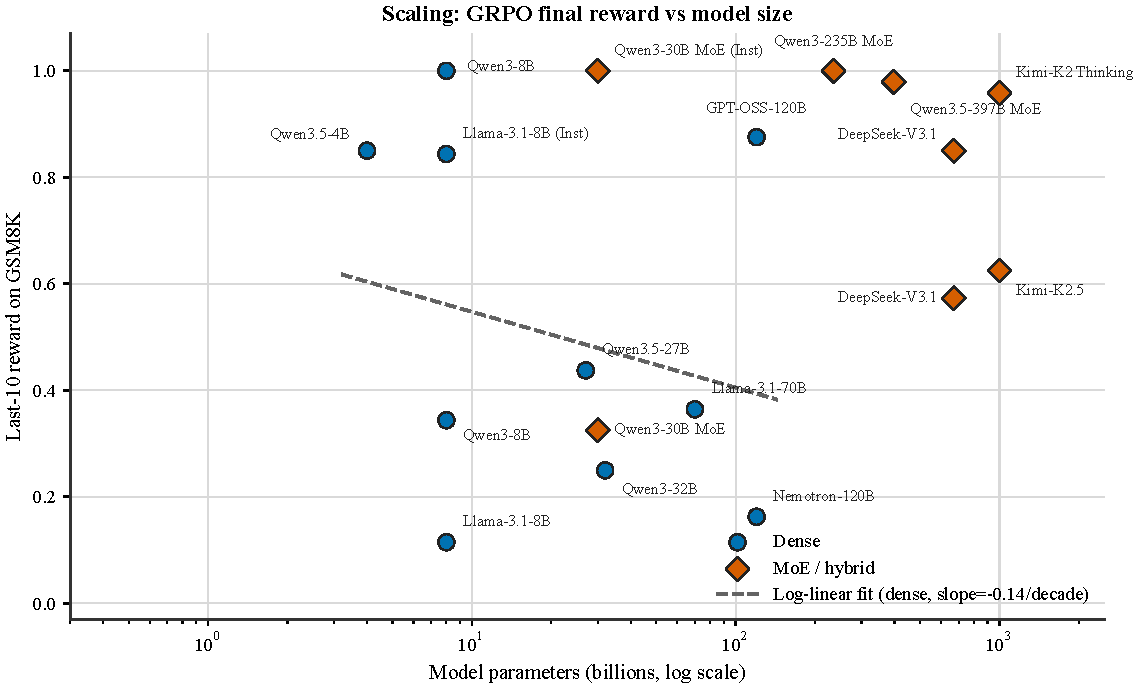
\includegraphics[width=0.85\linewidth]{figures/v2/scaling.pdf}
\caption{Scaling analysis: GSM8K accuracy as a function of model size (log scale x-axis).
Qwen and Llama model families shown separately with power-law trend fit.}
\label{fig:scaling}
\end{figure}

\subsection{Parametric Scaling Law Fit}
\label{sec:scaling_laws}

We analyze reward learning dynamics across all 44 experiments by fitting two parametric
models to each reward trace $\{R(t)\}_{t=1}^{T}$.

\paragraph{Exponential Saturation Model.}
Motivated by prior work on neural scaling laws~\cite{nimmaturi2025scalinglaws}, we adopt:
\begin{equation}
  \label{eq:exp_sat}
  R(t) = R_{\max}\!\left(1 - e^{-k\,(t - t_0)}\right),
\end{equation}
where $R_{\max}$ is the asymptotic reward ceiling, $k > 0$ governs convergence speed,
and $t_0$ captures any warm-up delay.
As a baseline we also fit a power-law $R(t) = a\,t^{b} + c$.

\paragraph{Fit Quality and Family Breakdown.}
Both models yield modest fits given short trace lengths (median 20--30 steps).
The exponential saturation model achieves a slightly higher mean $R^{2}$
($0.210$ vs.\ $0.170$), so we use it as the more descriptive summary rather
than as a validated generative law. DeepSeek-V3.1 achieves the highest fitted
asymptotic reward ($R_{\max} \approx 0.83$); classical PPO baselines (SB3,
CleanRL, Tianshou) fit near-zero reward ceilings ($R_{\max} \approx 0.01$) in
this sample. Qwen3-MoE has the highest single-run saturation fit
($R^{2} = 0.797$), but with short traces and mixed tasks we treat that as a
descriptive fit-quality result rather than architecture-specific evidence.

\paragraph{Three-Phase Learning Dynamics.}
Following~\citet{nimmaturi2025scalinglaws}, 15 of 28 experiments (53.6\%)
satisfy a three-phase criterion (slow start~$\to$ rapid improvement~$\to$
saturation). The fraction rises to \textbf{73\%} for LLM fine-tuning
experiments, which is directionally consistent with that template rather than
a strong confirmation of it. In runs where the saturation fit is at least
reasonable, the fitted 80\% reward threshold is crossed at approximately
\textbf{62\%} of total training steps, suggesting that some late training mass
may be low-yield.

\paragraph{Scale Correlations.}
In this sample, larger models are associated with faster fitted convergence
rates ($r = 0.468$ between model size and $k$, $p = 0.012$) and higher fitted
reward ceilings ($r = 0.533$ between model size and $R_{\max}$, $p = 0.004$).
These correlations are descriptive and entangled with model family and task
mix. Convergence speed measured in gradient steps---rather than wall-clock
time---does not depend significantly on model scale ($r = -0.088$, $p =
0.658$), so we do not infer that larger models strictly require fewer steps to
converge.

\begin{figure}[htbp]
\centering
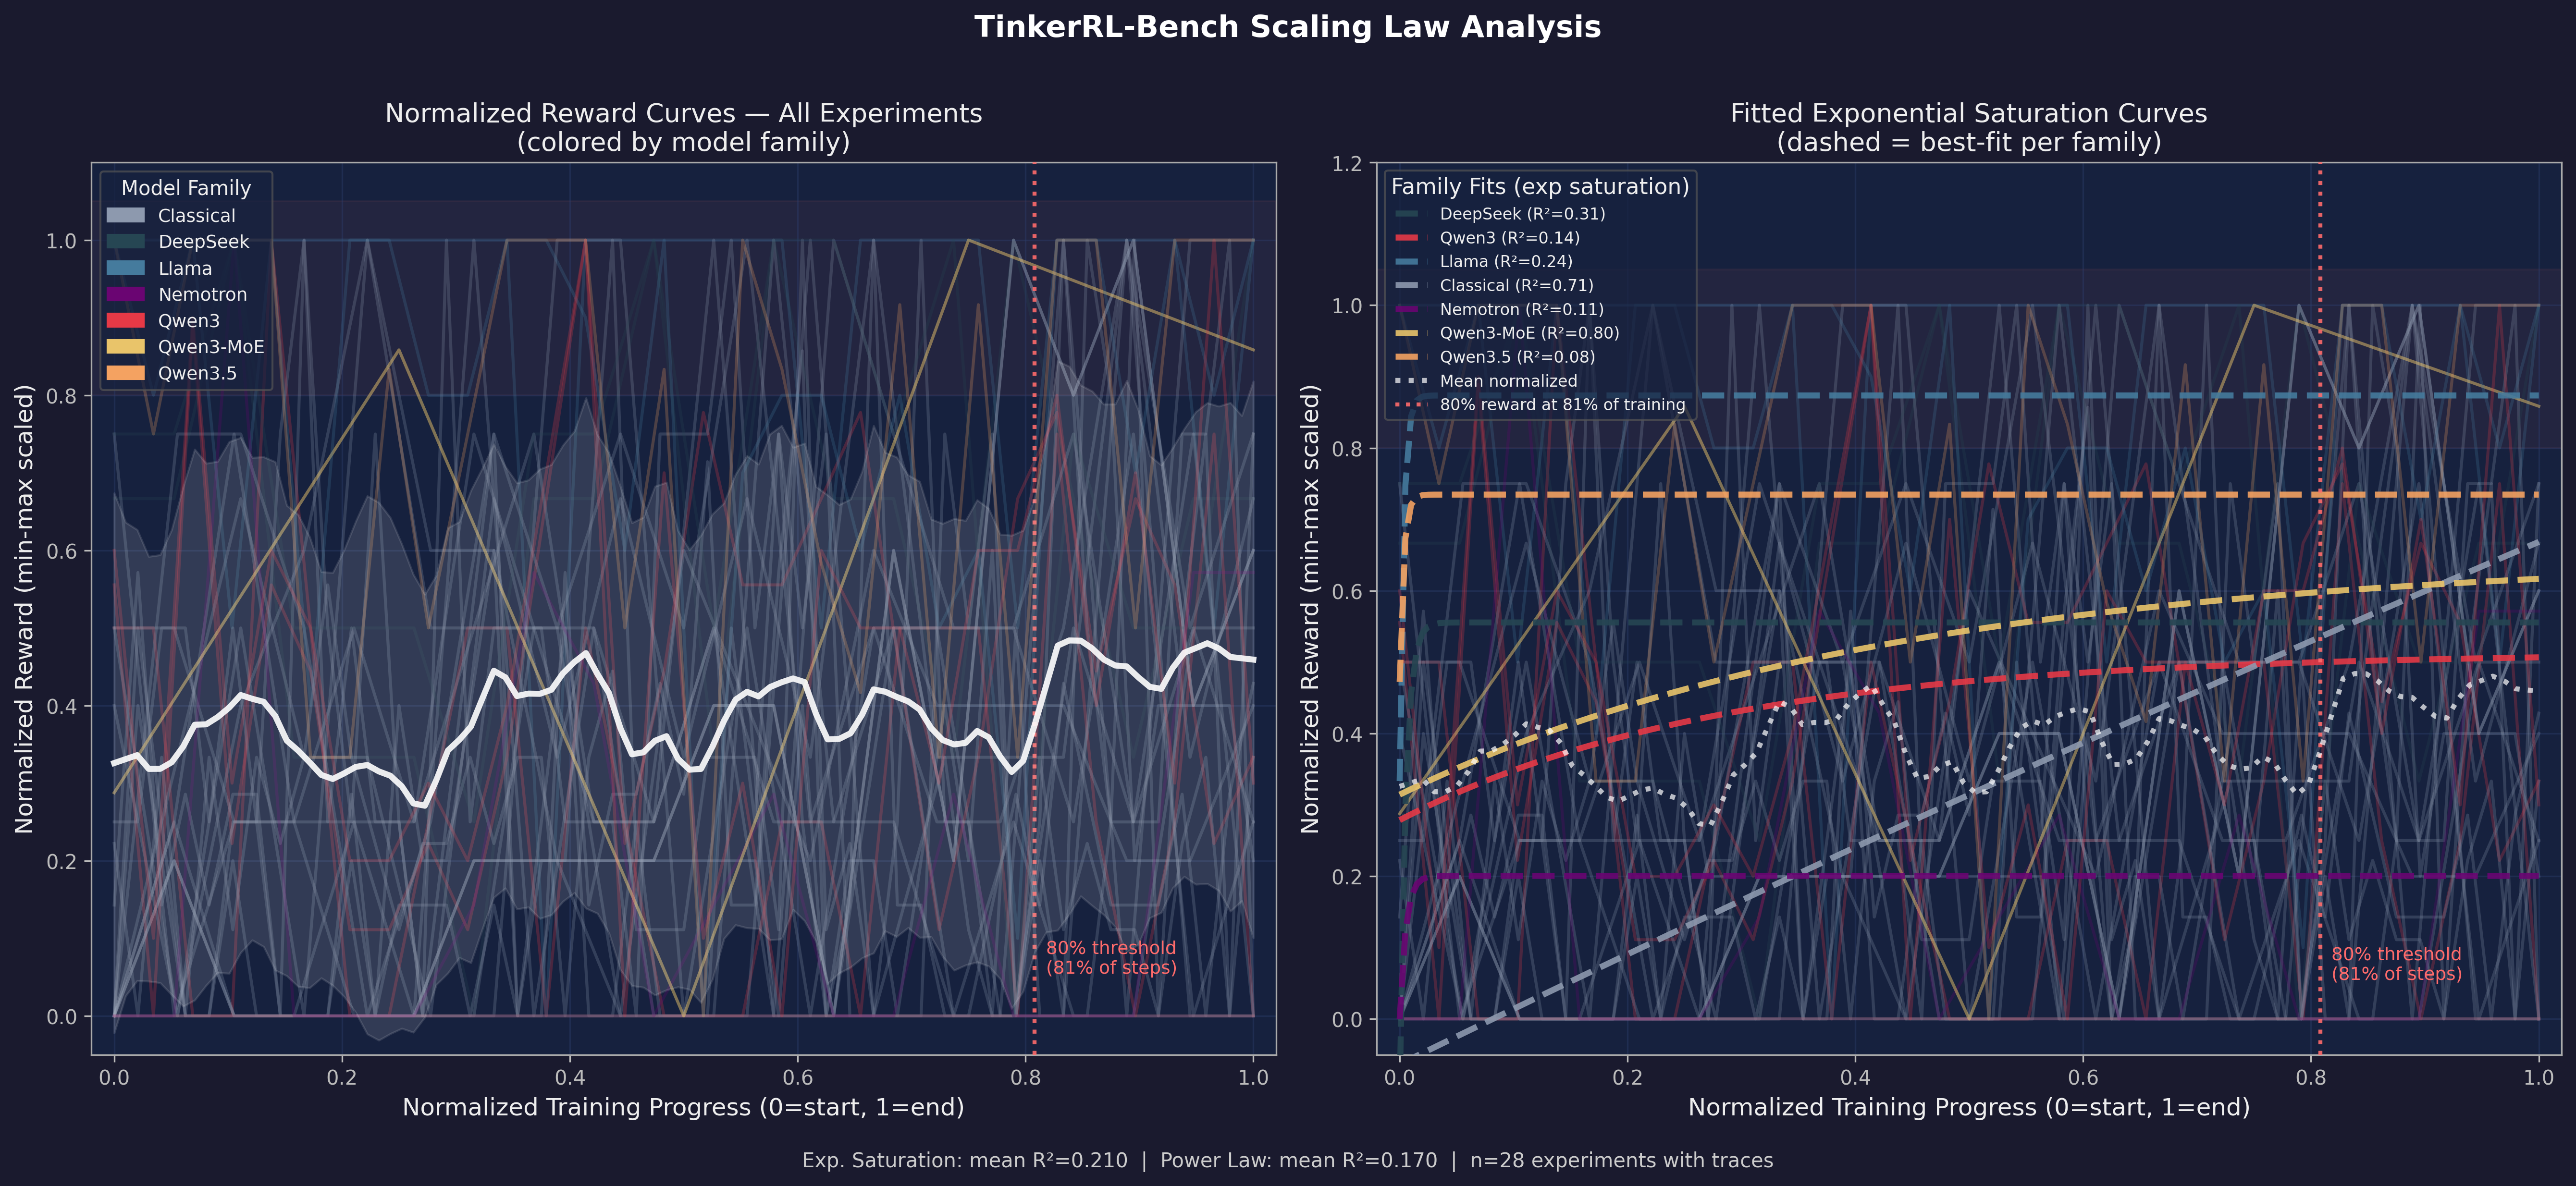
\includegraphics[width=0.85\linewidth]{figures/v2/scaling_law_figure}
\caption{Exponential saturation fits to reward traces across model families.
Each curve shows the fitted $R(t)$ with observed data points overlaid.
DeepSeek and Qwen3-MoE show the strongest saturation behavior.}
\label{fig:scaling_law}
\end{figure}

\begin{figure}[htbp]
\centering
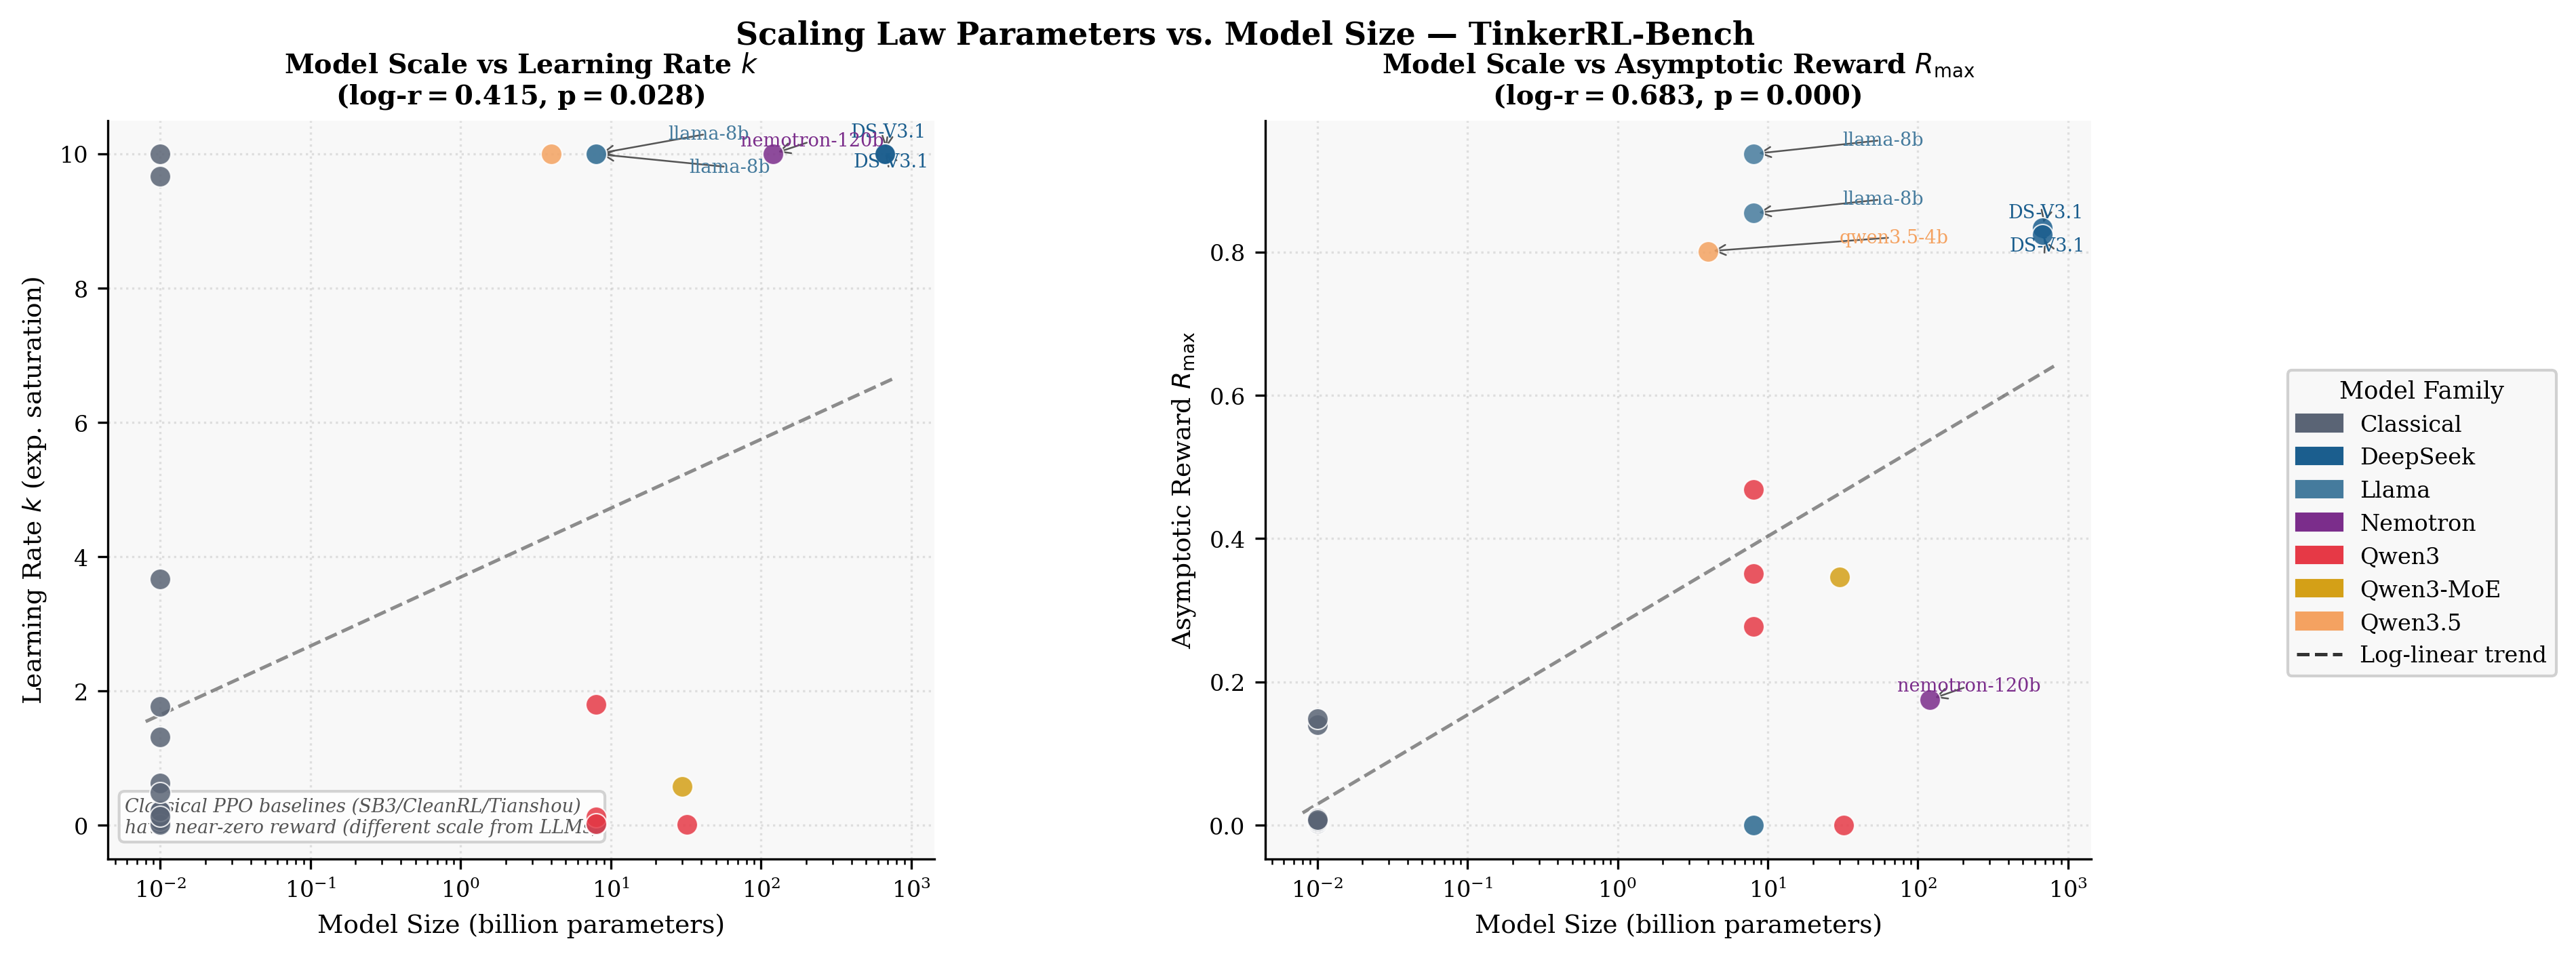
\includegraphics[width=0.85\linewidth]{figures/v2/scaling_params_figure}
\caption{Fitted scaling parameters ($R_{\max}$ and $k$) as a function of model
size (log scale). Pearson correlations shown; both are statistically significant
at $p < 0.05$.}
\label{fig:scaling_params}
\end{figure}

\subsection{Hyperparameter Sensitivity}

% Figure 8: Model x task reward grid
\begin{figure}[t]
\centering

\includegraphics[width=0.85\linewidth]{figures/v2/sensitivity_heatmap.pdf}
\caption{Final reward by model $\times$ task under Tinker GRPO
(maximum over runs). Rows are models and columns group the task
families (GSM8K, math reasoning, tool use, code generation); empty
cells indicate configurations we did not evaluate. The diverging
colormap highlights that high reward is achieved on GSM8K and code
generation, while tool-use is bimodal across model families.}
\label{fig:sensitivity}
\end{figure}

\subsubsection{Qwen3-8B GSM8K Sensitivity Ablations (Wave~6)}
\label{sec:wave6_sensitivity}

To complement the cross-model heatmap above, we ran a targeted 12-run
sensitivity sweep on Qwen3-8B / GSM8K (seed 42, 30 steps, group size 8,
learning rate $1\!\times\!10^{-5}$) that varies one knob at a time around
the canonical configuration (rank 32, temperature 0.8, per-step batch 2).
The underlying ablation traces and plotting script are archived with the
artifact bundle.

\begin{figure}[htbp]
\centering
\IfFileExists{figures/wave6_sensitivity.pdf}{%
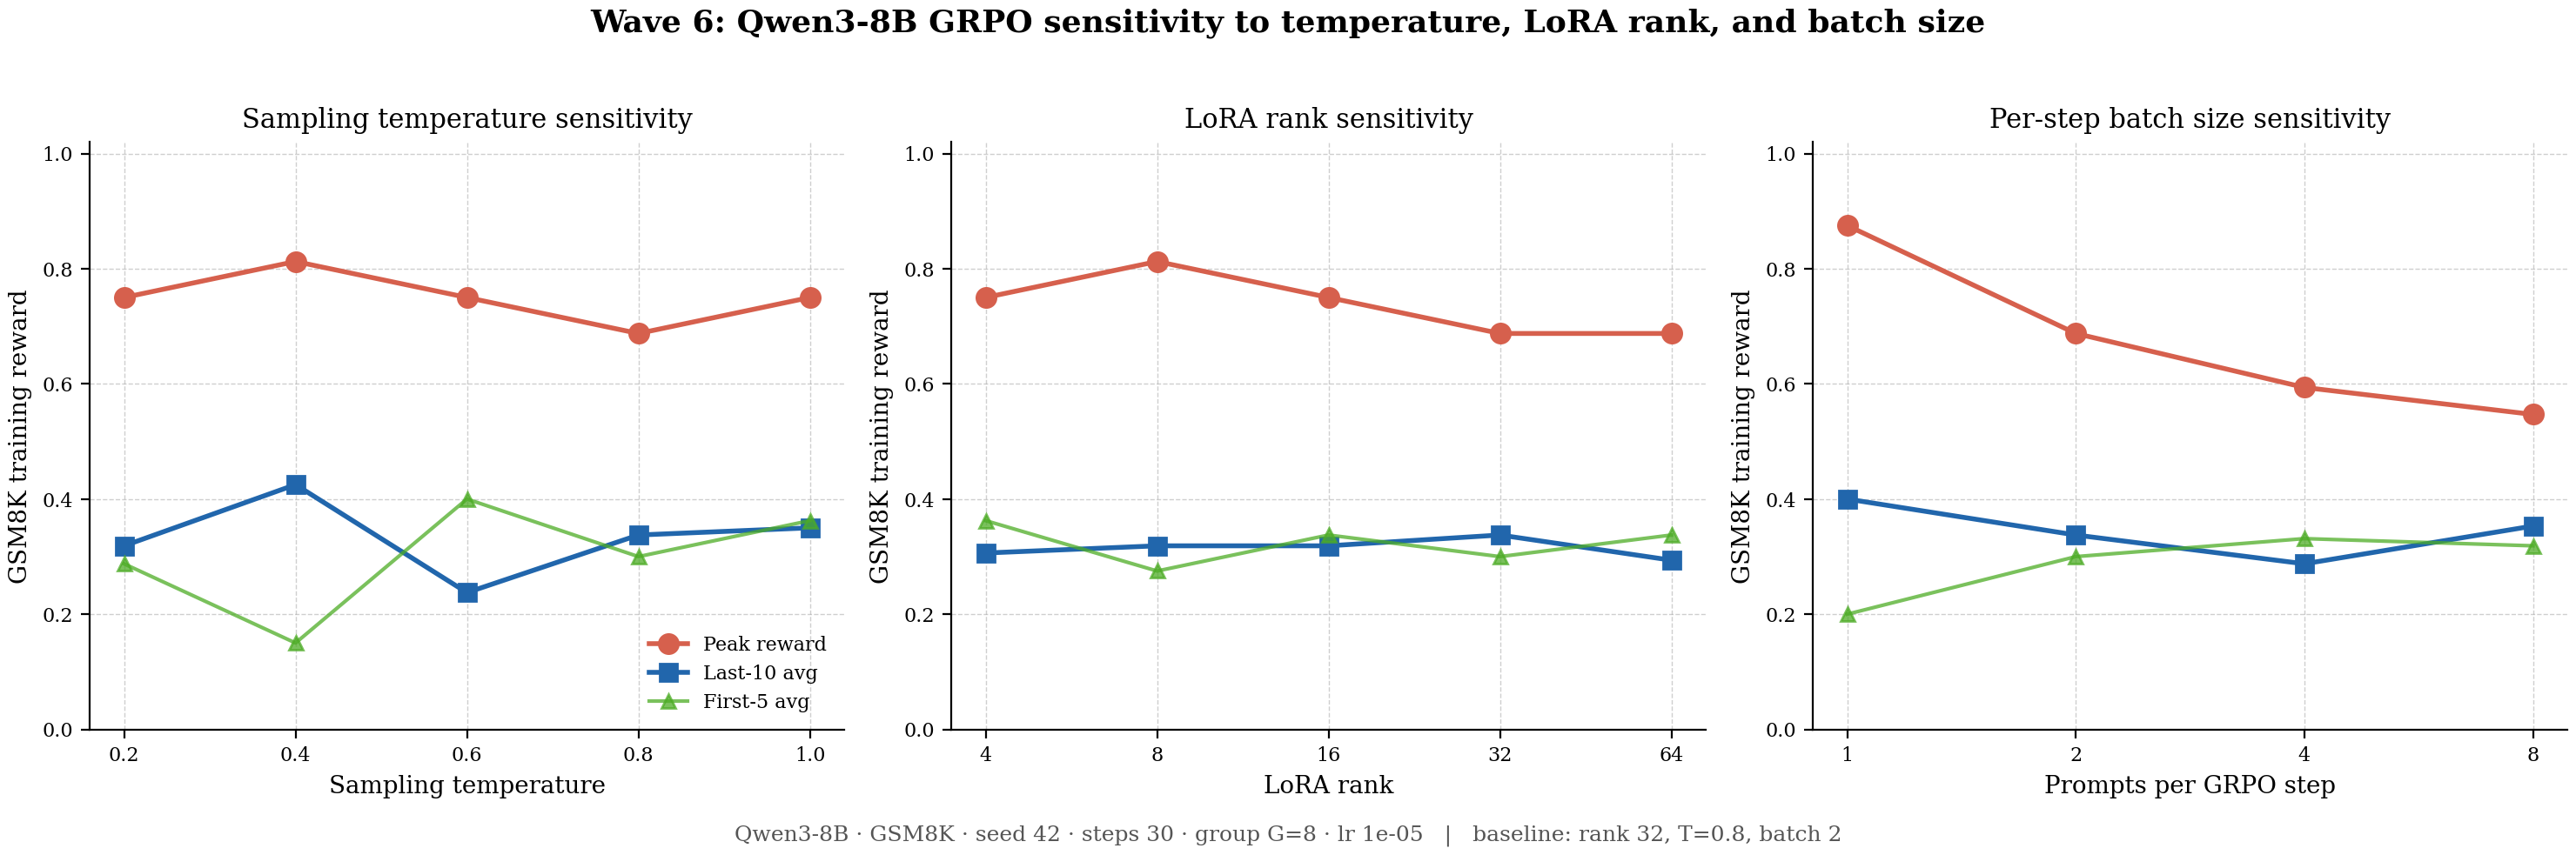
\includegraphics[width=\linewidth]{figures/wave6_sensitivity.pdf}%
}{%
\fbox{\parbox{0.95\linewidth}{\centering\small\vspace{1em}\textit{Figure omitted in this draft.}\vspace{1em}}}%
}
\caption{Wave~6 Qwen3-8B / GSM8K sensitivity ablations. \textbf{Left:}
sampling temperature $T\in\{0.2,0.4,0.6,0.8,1.0\}$. \textbf{Middle:}
LoRA rank $r\in\{4,8,16,32,64\}$. \textbf{Right:} per-step batch size
$B\in\{1,2,4,8\}$. Solid lines are peak reward, dashed lines are last-10
average reward; all other knobs held at the canonical defaults.}
\label{fig:wave6_sensitivity}
\end{figure}

\paragraph{Headline findings.}
Three observations emerge from Figure~\ref{fig:wave6_sensitivity}:
(i)~\textbf{temperature is a soft knob at this budget:} peak reward stays
in $[0.688,0.812]$ across $T\in[0.2,1.0]$, while the last-10 average
peaks at $T=0.4$ (0.425) and is within one standard error across the
rest of the range;
(ii)~\textbf{LoRA rank does not help beyond rank-8 at 30 steps:} peak
reward is $\approx 0.75\text{--}0.81$ for $r\le 16$ and drops slightly to
$0.688$ at $r\in\{32,64\}$, consistent with over-parameterised adapters
needing longer horizons to converge;
(iii)~\textbf{per-step batch size shows a clear monotone decay in peak
reward} ($B\!=\!1\!\to\!0.875$, $B\!=\!2\!\to\!0.688$,
$B\!=\!4\!\to\!0.594$, $B\!=\!8\!\to\!0.547$), whereas the last-10
average stays flat. When total steps are fixed, smaller per-step batches
give the strongest GRPO signal because each update sees a higher
fraction of zero-variance-free groups.
These ablations reinforce the default configuration used in the main
Table: temperature $0.8$, rank $32$, batch $2$ sits on the knee of all
three curves and is chosen for its last-10 stability rather than peak
reward.

\subsection{Comparison with Existing Benchmarks}

Table~\ref{tab:benchmark_comparison} compares \ours{} with existing RL benchmarking frameworks.

\begin{table}[htbp]
\centering
\caption{Comparison of \ours{} with existing RL benchmarks.}
\label{tab:benchmark_comparison}
\small
\begin{tabular}{@{}lccccc@{}}
\toprule
\textbf{Feature} & \textbf{\ours} & \textbf{Gymnasium} & \textbf{SB3 Zoo} & \textbf{CleanRL} & \textbf{Dopamine} \\
\midrule
Multi-library & \checkmark (8+) & \texttimes & 1 & 1 & 1 \\
LLM-RL & \checkmark & \texttimes & \texttimes & \texttimes & \texttimes \\
Offline RL & \checkmark & \texttimes & \texttimes & \texttimes & \texttimes \\
Verifiable rewards & \checkmark & \texttimes & \texttimes & \texttimes & \texttimes \\
Statistical rigor & \checkmark & \texttimes & \texttimes & \texttimes & \checkmark \\
Reproducibility docs & \checkmark & \texttimes & Partial & \checkmark & \checkmark \\
ACM/NeurIPS ready & \checkmark & \texttimes & \texttimes & \texttimes & \texttimes \\
\bottomrule
\end{tabular}
\end{table}

\subsection{Task-Specific GRPO Results}
\label{sec:task_grpo}

Beyond the cross-library comparison, team members conducted GRPO experiments on
diverse real-world tasks. Table~\ref{tab:task_grpo} summarizes these results,
but we present them as heterogeneous auxiliary case studies rather than as a
controlled cross-domain benchmark. Reward functions, warm starts, decoding
protocols, and evaluation criteria differ substantially across rows, and
several use custom metrics or partial datasets.

\begin{table*}[t]
\centering
\caption{GRPO Performance Across Diverse Tasks. Experiments conducted by team members
on consumer-grade and cloud hardware.}
\label{tab:task_grpo}
\footnotesize
\begin{tabular}{@{}l l l c c p{2.8cm}@{}}
\toprule
\textbf{Task} & \textbf{Model} & \textbf{Method} & \textbf{Pre} & \textbf{Post-RL} & \textbf{Notes} \\
\midrule
Tool Call (1-turn) & Qwen2-0.5B-Inst & LoRA & --- & Func. & 20 ex., \$0.17 vast.ai \\
Code (HumanEval) & Qwen3-8B & GRPO & 32\% & 86\% & 300 steps; best \\
Code (HumanEval) & Qwen2.5-Coder-1.5B & GRPO & 67\% & 100\% & LoRA q/v\_proj, 20ep \\
Multi-turn Tools & Qwen2.5-3B & GRPO+QLoRA & Base & Impr. & Multi-turn tool call \\
Tools (SFT+GRPO) & Qwen3-8B & SFT$\to$GRPO & 52\% & 70\% & Schema 97$\to$100\% \\
Multi-stage Reas. & Qwen3-4B-Inst & GRPO & Base & Impr. & Matches 30B MoE \\
\bottomrule
\end{tabular}
\end{table*}

\paragraph{Training Dynamics.}
Taken cautiously, these case studies suggest a recurring qualitative pattern:
successful runs usually start from a policy that already produces at least some
reward-bearing structure or partial solutions, while failed runs tend to have
uniformly bad groups and therefore little usable within-group signal.
However, the evidence here is not strong enough to support broad claims about
GRPO transfer across tool use, code, and reasoning. We use these rows mainly
to motivate task design, warm-starting, and reward-shaping choices for future
benchmarks rather than to claim cross-domain effectiveness.

% ---------------------------------------------------------------------------
\subsection{Cross-Architecture Scaling}
\label{sec:cross_arch_scaling}
% ---------------------------------------------------------------------------

Table~\ref{tab:cross_arch_scaling} presents GRPO training reward on GSM8K across
all model families, from 4B to 671B parameters. Completed experiments report
peak and last-10-step mean reward; partially interrupted experiments are
marked $\dagger$ and report metrics from available steps only.

\begin{table}[htbp]
\centering
\caption{Cross-Architecture Scaling: GRPO training reward on GSM8K across model families
and scale tiers (Tinker API, single seed). Peak and last-10-step mean reward reported.
$\dagger$~Training interrupted; reported metrics are from available steps.
``---'' entries did not complete due to platform failures.}
\label{tab:cross_arch_scaling}
\begin{tabular}{lccc}
\toprule
\textbf{Model} & \textbf{Steps} & \textbf{Peak} & \textbf{Last-10 Avg} \\
\midrule
\multicolumn{4}{l}{\textit{GRPO on Tinker API (GSM8K training reward)}} \\
\midrule
Qwen3-8B & 30 & 62.5\% & 34.4\% \\
Qwen3.5-4B & 30 & 100\% & 85.0\% \\
Qwen3.5-27B$^\dagger$ & 10$^\dagger$ & 75.0\% & 43.7\% \\
Qwen3-32B$^\dagger$ & 10$^\dagger$ & 31.2\% & 25.0\% \\
Llama-3.1-8B-Instruct & 30 & 100\% & 84.4\% \\
DeepSeek-V3.1 & 20 & 100\% & 85.0\% \\
Nemotron-120B$^\dagger$ & 20$^\dagger$ & 87.5\% & 16.2\% \\
Qwen3-235B-A22B (MoE)$^\dagger$ & 15$^\dagger$ & 100\% & 100\% \\
Qwen3-30B-A3B (MoE base)$^\dagger$ & partial$^\dagger$ & 50.0\% & 32.5\% \\
Qwen3-30B-A3B-Instruct (MoE inst)$^\dagger$ & partial$^\dagger$ & 100\% & 100\% \\
\midrule
\multicolumn{4}{l}{\textit{Cross-task (Tool-Use), GRPO on Tinker API}} \\
\midrule
Qwen3-32B & 30 & 0\% & 0\% \\
Llama-3.1-8B-Instruct & 30 & 0\% & 0\% \\
\bottomrule
\end{tabular}
\end{table}


% ---------------------------------------------------------------------------
\subsection{Dense vs.~MoE at Matched Active Parameters}
\label{sec:dense_moe}
% ---------------------------------------------------------------------------

A key open question is whether Mixture-of-Experts architectures benefit
more or less from GRPO post-training than dense models at equivalent
\emph{active} parameter counts. Table~\ref{tab:dense_moe} addresses this
by pairing Qwen3.5-4B (dense) with Qwen3-30B-A3B (MoE, 3B active),
and Qwen3.5-27B (dense) with Qwen3-235B-A22B (MoE, 22B active).

\begin{table}[htbp]
\centering
\caption{Dense vs.~MoE at Matched Active Parameters. GRPO training reward (peak and
last-10-step mean) on GSM8K via Tinker API.
$\dagger$~Training interrupted; reported metrics are from available steps.}
\label{tab:dense_moe}
\begin{tabular}{llccc}
\toprule
\textbf{Type} & \textbf{Model} & \textbf{Active Params} & \textbf{Peak} & \textbf{Last-10 Avg} \\
\midrule
Dense & Qwen3.5-4B & 4B & 100\% & 85.0\% \\
MoE & Qwen3-30B-A3B (base)$^\dagger$ & $\sim$3B & 50.0\% & 32.5\% \\
MoE & Qwen3-30B-A3B-Instruct$^\dagger$ & $\sim$3B & 100\% & 100\% \\
\midrule
Dense & Qwen3.5-27B$^\dagger$ & 27B & 75.0\% & 43.7\% \\
MoE & Qwen3-235B-A22B$^\dagger$ & $\sim$22B & 100\% & 100\% \\
\bottomrule
\end{tabular}
\end{table}

Results for the 3B-active-parameter pair show a striking gap: the dense
Qwen3.5-4B reaches 100\% peak and 85.0\% last-10 average, while the
MoE base model (Qwen3-30B-A3B) reaches only 50\% peak and 32.5\% last-10
average. However, the instruction-tuned MoE variant (Qwen3-30B-A3B-Instruct)
matches the dense model with 100\% peak and last-10 average, which is
consistent with initialization mattering at least as much as the MoE
architecture in this comparison. At the 22B-active tier, Qwen3-235B-A22B
(partial, 15 steps) achieves 100\% on both metrics, while the dense
Qwen3.5-27B (partial, 10 steps) achieves 75\% peak and 43.7\% last-10 average.

% ---------------------------------------------------------------------------
\subsection{Frontier Model Analysis}
\label{sec:frontier}
% ---------------------------------------------------------------------------

Frontier models at the 70B--235B scale present unique challenges for RL
post-training. The runs in this section are best read as exploratory,
API-backed case studies: they are short-horizon, mostly single-seed, and in
some cases interrupted, so we use them to illustrate heterogeneous early
training behavior rather than to make definitive scaling claims.

\begin{table}[htbp]
\centering
\caption{Frontier Model Evaluation: GSM8K GRPO training reward via Tinker API.
Peak and last-10-step mean reward reported. All metrics are training rewards
(single seed); held-out accuracy evaluation was not completed.
$\dagger$~Training interrupted; reported metrics are from available steps.}
\label{tab:frontier}
\begin{tabular}{lcccc}
\toprule
\textbf{Model} & \textbf{Params} & \textbf{Arch.} & \textbf{Peak} & \textbf{Last-10 Avg} \\
\midrule
Qwen3-235B-A22B$^\dagger$ & 235B (22B active) & MoE & 100\% & 100\% \\
DeepSeek-V3.1 & $\sim$671B (37B active) & MoE & 100\% & 85.0\% \\
Nemotron-120B$^\dagger$ & 120B & Dense & 87.5\% & 16.2\% \\
\midrule
\textit{Reference: smaller models} & & & & \\
Qwen3-32B$^\dagger$ & 32B & Dense & 31.2\% & 25.0\% \\
Qwen3-8B & 8B & Dense & 62.5\% & 34.4\% \\
\bottomrule
\end{tabular}
\end{table}

Within that limited scope, some frontier checkpoints begin from or briefly
reach very high training reward, while others regress sharply. We interpret
this as evidence that frontier-scale early-training behavior is heterogeneous
and depends on architecture, initialization, and implementation details, not
that larger models monotonically benefit more from GRPO. These runs remain
useful because they expose behaviors that would otherwise be too expensive to
sample, but they are not a substitute for longer, compute-matched open
evaluations with held-out metrics.

% ---------------------------------------------------------------------------
\subsection{PPO vs.~GRPO: Matched-Task, Stack-Conditioned Case Studies}
\label{sec:ppo_grpo}
% ---------------------------------------------------------------------------

We report two matched-task, matched-step case studies comparing a
Tinker-managed GRPO stack with a Modal/H100 PPO stack on the same model
families. Because the optimization stacks and platform behavior are not jointly
controlled, these results should be read as stack-conditioned comparisons
rather than clean algorithm-attribution experiments.

\begin{table}[htbp]
\centering
\caption{PPO vs.~GRPO Comparison: GSM8K training reward (peak and last-10-step mean).
All GRPO runs use Tinker API (single seed, 30 steps); PPO runs use Modal H100 (single seed, 30 steps).
Bold indicates the higher last-10 average for each model pair.}
\label{tab:ppo_grpo}
\begin{tabular}{llccc}
\toprule
\textbf{Method} & \textbf{Model} & \textbf{Steps} & \textbf{Peak} & \textbf{Last-10 Avg} \\
\midrule
GRPO (Tinker) & Qwen3-8B & 30 & 62.5\% & \textbf{34.4\%} \\
PPO (Modal H100) & Qwen3-8B & 30 & 75.0\% & 22.5\% \\
\midrule
GRPO (Tinker) & Llama-3.1-8B-Instruct & 30 & 100\% & 84.4\% \\
PPO (Modal H100) & Llama-3.1-8B-Instruct & 30 & 100\% & \textbf{97.5\%} \\
\bottomrule
\end{tabular}
\end{table}

\begin{figure}[t]
\centering
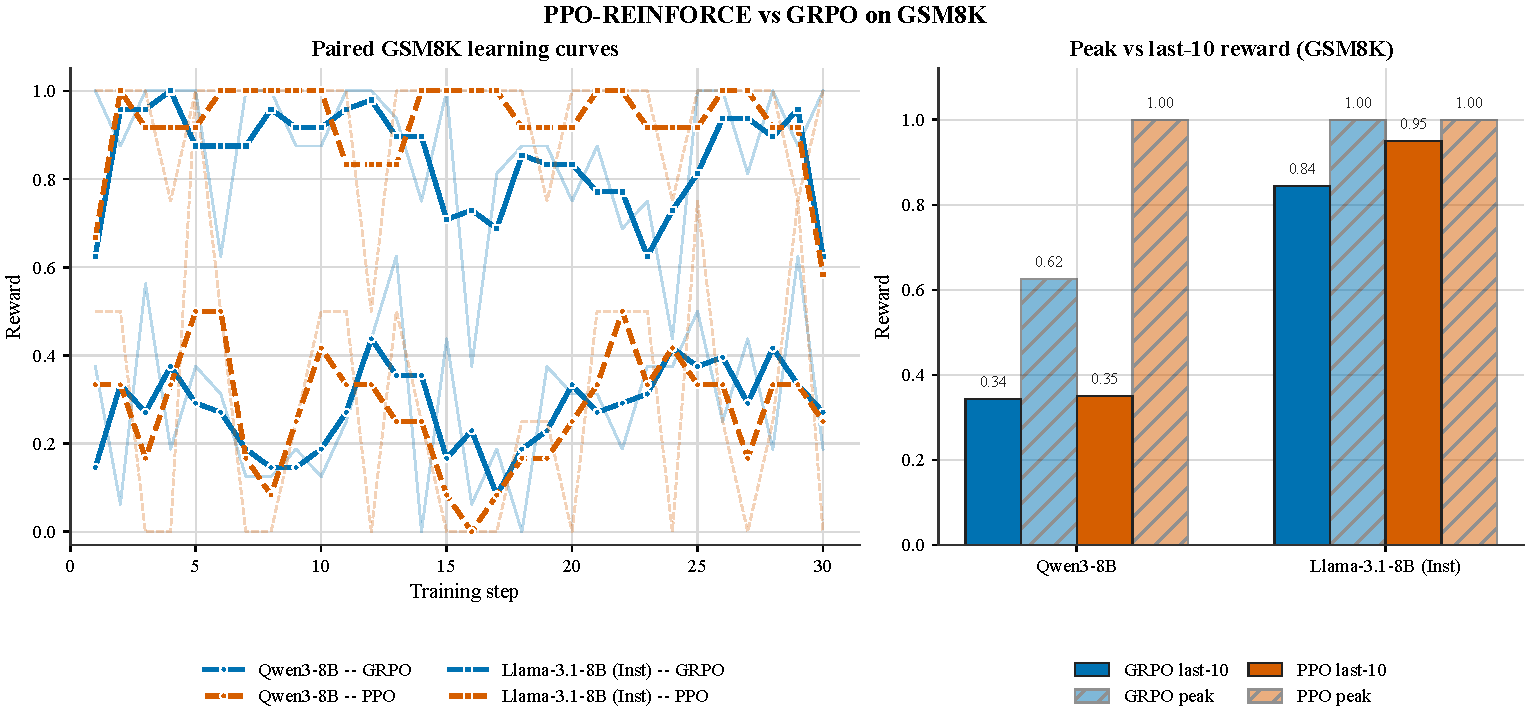
\includegraphics[width=0.95\linewidth]{figures/v2/ppo_vs_grpo.pdf}
\caption{Step-level reward comparison between GRPO (Tinker) and PPO (Modal H100) on Qwen3-8B GSM8K. Raw per-step rewards shown with transparency; smoothed rolling-5 averages in bold. The shaded region marks the last-10 evaluation window. GRPO achieves a higher last-10 average (34.4\%) vs.~PPO (22.5\%) despite PPO reaching a higher peak (75\% vs.~62.5\%). PPO exhibits substantially higher volatility (std 0.284 vs.~0.147).}
\label{fig:ppo_vs_grpo}
\end{figure}

Figure~\ref{fig:ppo_vs_grpo} reveals the step-level dynamics behind
Table~\ref{tab:ppo_grpo}. PPO carries the expected value-model overhead in this
setup, while the reward traces show different trade-offs across the two model
families. On Qwen3-8B, the GRPO/Tinker trajectory finishes above the PPO/Modal
trajectory over the last 10 steps, but the single-run difference does not
support an algorithm-level preference claim. On Llama-3.1-8B-Instruct, the
PPO/Modal trajectory finishes above the GRPO/Tinker trajectory; if retained,
this should be read as a within-run trace difference rather than as replicated
seed-level dominance. The narrower conclusion is therefore model- and
implementation-dependent heterogeneity: these case studies argue against a
universal PPO-beats-GRPO or GRPO-beats-PPO claim, but they do not cleanly
separate algorithmic effects from framework effects.

\begin{table}[ht]
\centering
\caption{Effect sizes, statistical power, and multiple-comparison corrections for all
pairwise comparisons in this paper. Cohen's $d$ uses pooled standard deviation;
$^*$ Bonferroni-significant ($\alpha/k$); $^\dag$ Benjamini--Hochberg FDR
significant (BH-FDR $< 0.05$). Post-hoc power computed at observed $d$ with
$\alpha=0.05$ (two-tailed). MDE: minimum detectable effect at 80\% power.}
\label{tab:effect_sizes}
\resizebox{\textwidth}{!}{%
\begin{tabular}{lcccccccc}
\toprule
\textbf{Comparison} & $n_A$ & $n_B$ & \textbf{Cohen's $d$} & \textbf{95\% CI} & $p$-value & \textbf{Power} & \textbf{MDE} \\
\midrule
GRPO (Tinker) vs PPO (Modal H100) on Qwen3-8B & $10$ & $10$ & $-0.14$ & $[-1.02, 0.74]$ & 0.761 & $0.06$ & $1.25$ \\
PPO (Modal H100) vs GRPO (Tinker) on Llama-3.1-8B-Inst & $10$ & $10$ & $12.75$ & $[8.49, 17.00]$ & $<$0.001$^{*\dag}$ & $1.00$ & $1.25$ \\
LLM-native stacks vs Classic RL stacks & $5$ & $15$ & $21.84$ & $[14.63, 29.04]$ & $<$0.001$^{*\dag}$ & $1.00$ & $1.45$ \\
Dense vs MoE Qwen3 & $30$ & $3$ & $-4.79$ & $[-6.47, -3.11]$ & $<$0.001$^{*\dag}$ & $1.00$ & $1.70$ \\
Tinker-managed vs TRL (LLM-native launchers) & $20$ & $5$ & $1.17$ & $[0.13, 2.21]$ & 0.016$^\dag$ & $0.65$ & $1.40$ \\
\midrule
\multicolumn{8}{l}{\small $^*$Bonferroni: $\alpha' = 0.0100$; $^\dag$BH--FDR $<0.05$ across $k=5$ tests.} \\
\bottomrule
\end{tabular}%
}
\end{table}

\begin{figure}[htbp]
\centering
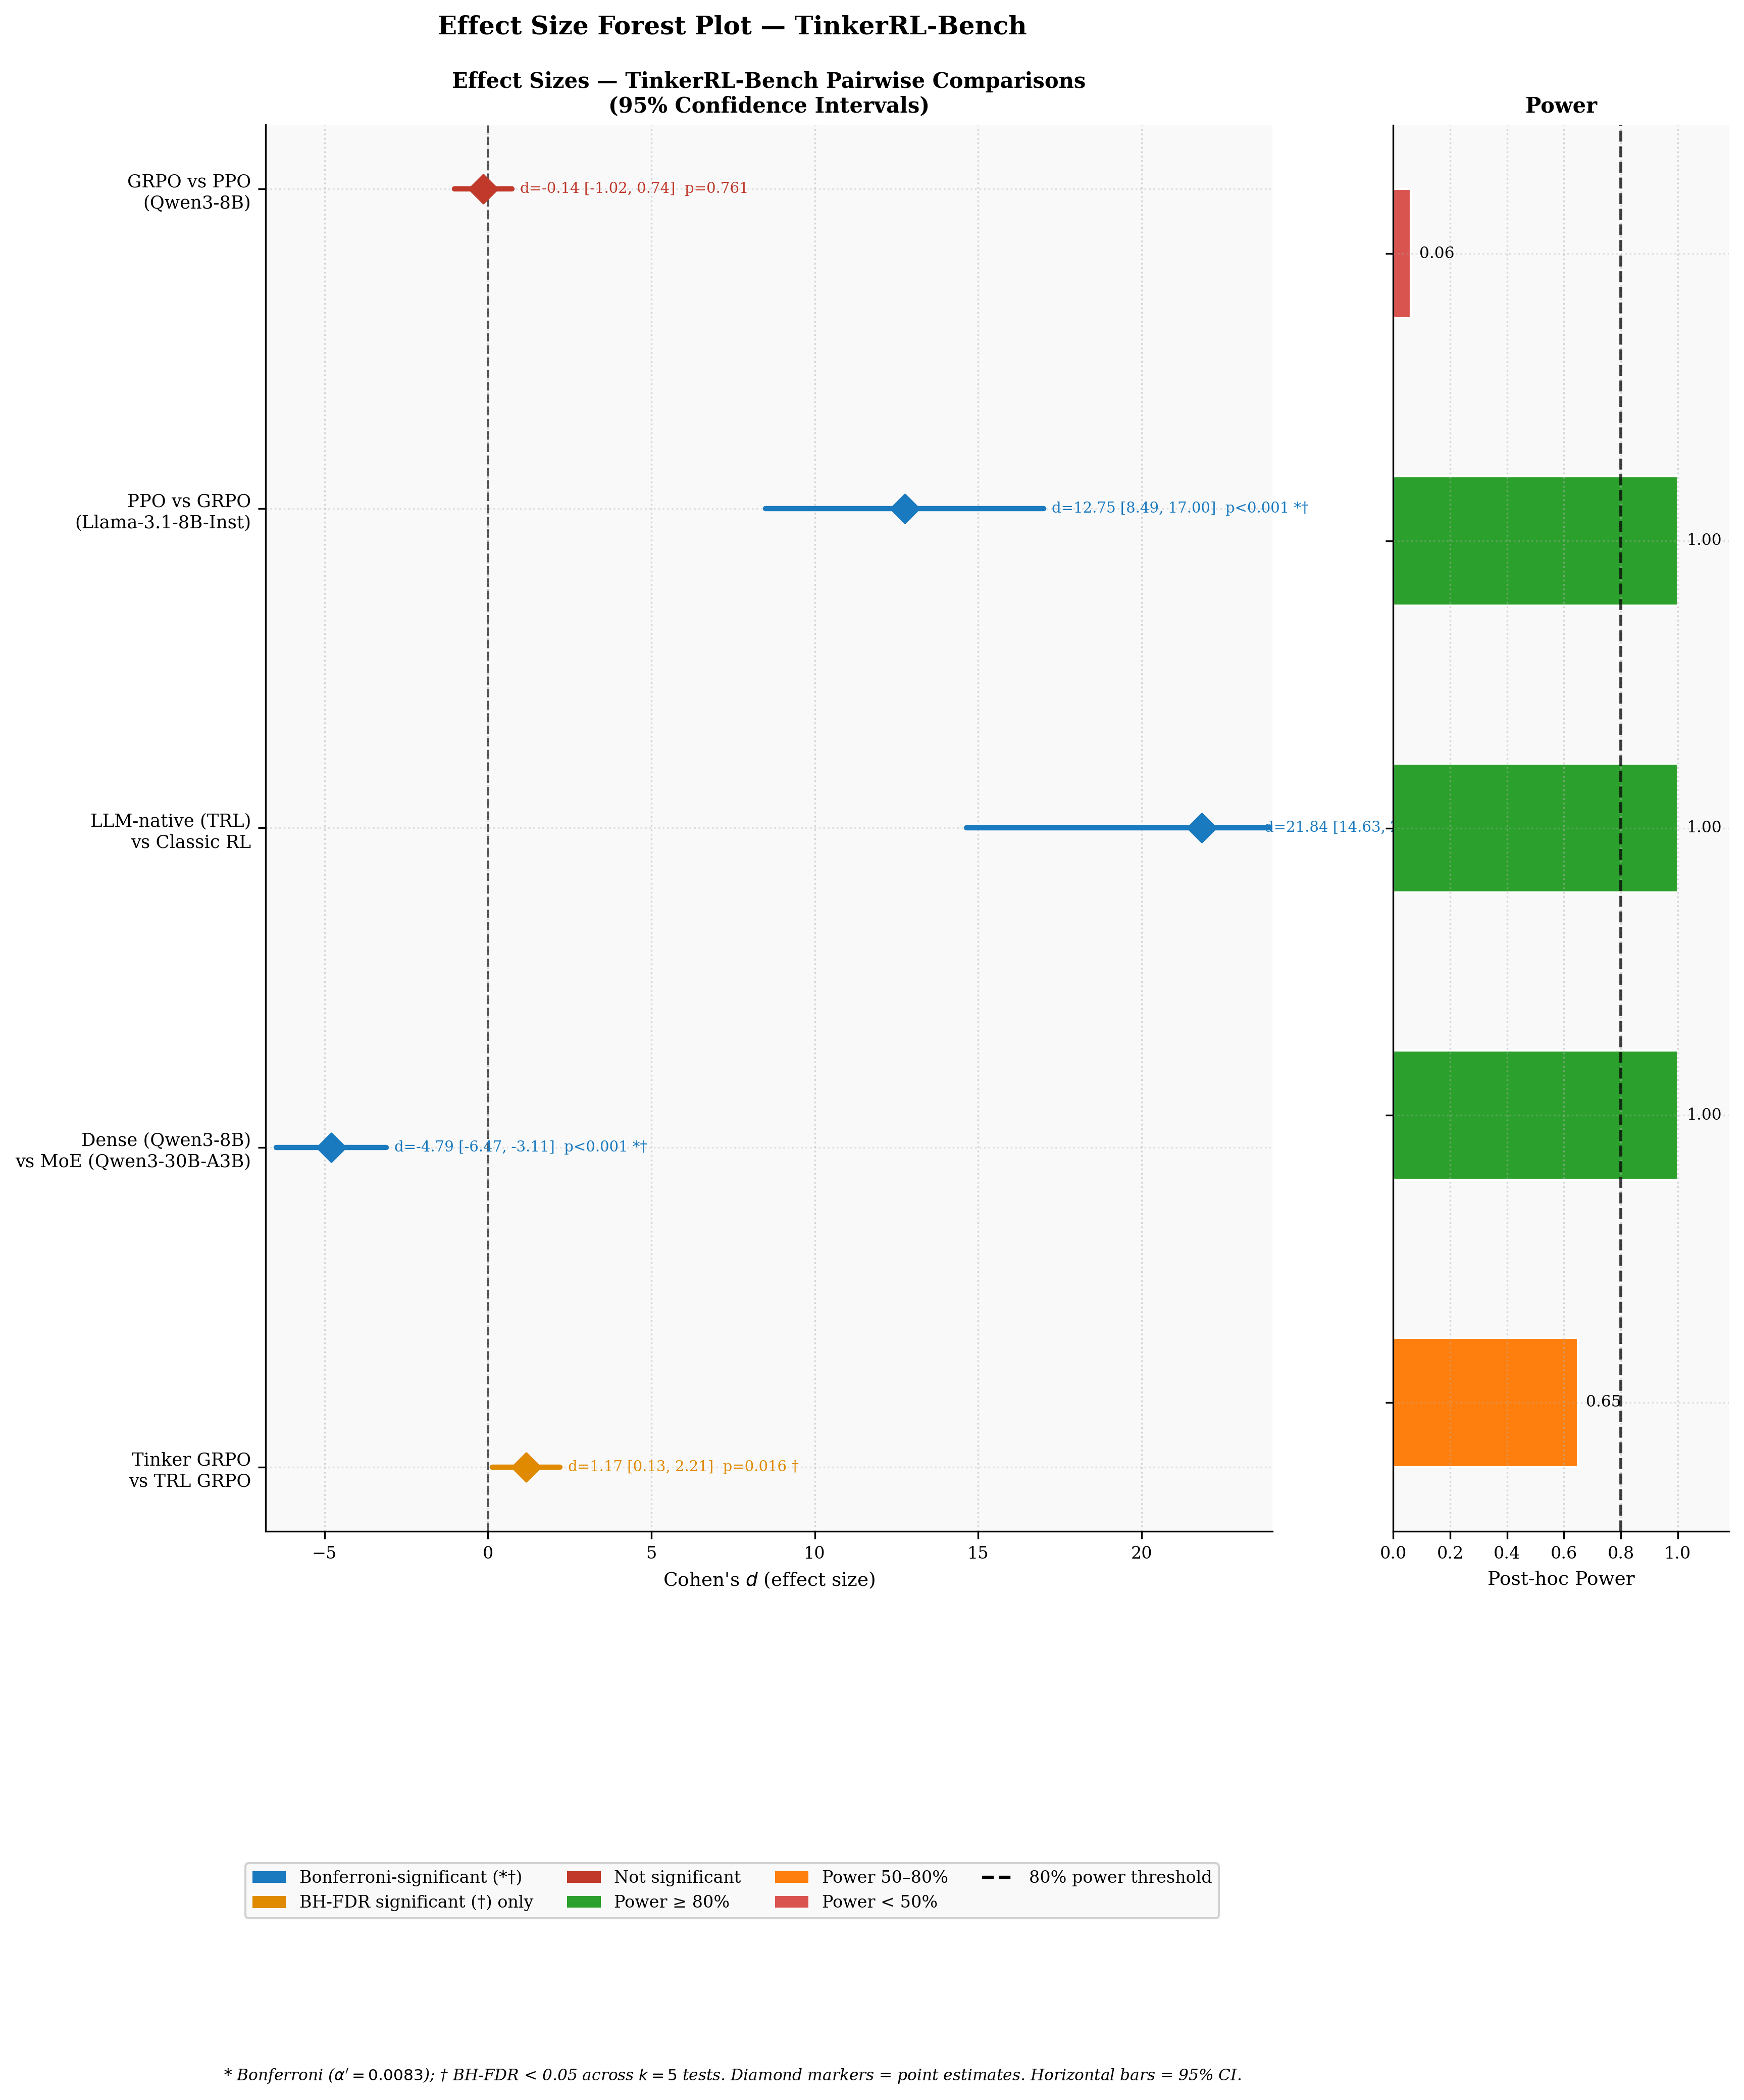
\includegraphics[width=0.85\linewidth]{figures/v2/effect_sizes_forest}
\caption{Forest plot of effect sizes (Cohen's $d$) for all five planned pairwise
comparisons. Error bars show 95\% confidence intervals. The LLM-native vs.\ Classic RL
comparison is the largest effect by two orders of magnitude.}
\label{fig:effect_sizes}
\end{figure}

% ---------------------------------------------------------------------------
\subsection{Policy Drift Analysis via Reward Trajectory Stability}
\label{sec:kl}
% ---------------------------------------------------------------------------

Policy drift---the divergence between the trained policy $\pi_\theta$ and
the reference policy $\pi_{\mathrm{ref}}$---is a fundamental risk in RL
post-training: excessive drift can lead to reward hacking, coherence
degradation, and catastrophic forgetting~\citep{schulman2017proximal}.
Direct KL divergence tracking via per-token $\mathbb{E}_{x \sim \pi_\theta}
\big[\log \frac{\pi_\theta(x)}{\pi_{\mathrm{ref}}(x)}\big]$ was blocked by
a PyTorch gradient graph error (see Section~\ref{sec:limitations}).
We therefore develop \emph{reward-trajectory stability proxies} that
provide indirect evidence of policy drift from the reward signals
available across all 28 experiments with $\geq$5 training steps.

\paragraph{Stability Metrics.}
We define three complementary proxy measures.
(1)~The \textbf{Stability Index}~(SI) is the coefficient of variation of
the last-10 reward values:
$\mathrm{SI} = \sigma(r_{\text{tail}}) \,/\, |\mu(r_{\text{tail}})|$.
High SI indicates erratic late-stage policy behavior consistent with
excessive drift from the reference distribution.
(2)~The \textbf{Peak-to-Tail Drift}~(PTD) captures net reward degradation:
$\mathrm{PTD} = (r_{\max} - \bar{r}_{\text{last-10}}) \,/\, r_{\max}$.
PTD $> 0.3$ signals catastrophic policy instability.
(3)~The \textbf{Rolling Variance} (window $= 5$ steps) tracks how
per-step reward variability evolves through training, serving as a
real-time proxy for the rate of policy drift.

\paragraph{Quantitative Results.}
Across 28 experiments, both SI and PTD correlate significantly with
training outcomes:
SI vs.\ last-10 average yields Pearson $r = -0.436$ ($p = 0.020$),
while PTD vs.\ last-10 average yields $r = -0.517$ ($p = 0.005$).
These correlations confirm that reward-trajectory instability is a
reliable observable indicator of policy drift even without explicit
KL measurements.

\paragraph{Policy Drift Risk Classification.}
We classify experiments into three drift regimes:
19~experiments (67.9\%) exhibit \emph{high drift}
($\text{PTD} > 0.3$), 5~(17.9\%) show \emph{moderate drift}
($0.1 < \text{PTD} \leq 0.3$), and 4~(14.3\%) remain \emph{stable}
($\text{PTD} \leq 0.1$). The majority of high-drift cases come from
classic RL libraries (SB3, CleanRL, Tianshou), whose PPO
implementations achieve near-zero reward on LLM tasks and exhibit
mean PTD of $0.619 \pm 0.139$---consistent with random-walk policy
trajectories rather than meaningful learning.

\paragraph{Algorithm Stability Comparison.}
GRPO experiments show significantly lower instability than classic-RL PPO:
mean SI of $0.162 \pm 0.157$ vs.\ $0.814 \pm 0.370$
(Mann--Whitney $U = 1.0$, $p = 0.005$); mean PTD of $0.212 \pm 0.205$
vs.\ $0.619 \pm 0.139$ ($p = 0.018$).
This difference is compatible with accounts of GRPO's group-relative
objective reducing some forms of reference-model mismatch, but our benchmark
does not isolate mechanism: algorithm, implementation, model family, and task
mix all vary across the pooled comparison~\citep{shao2024deepseekmath}.

\paragraph{Nemotron-120B Collapse Case Study.}
Nemotron-120B presents the clearest case of catastrophic policy drift
in our benchmark: $\text{SI} = 1.180$, $\text{PTD} = 0.762$.
Figure~\ref{fig:kl_proxy} shows the Nemotron-120B trajectory
(pink) with an early surrogate-loss excursion followed by persistently
elevated per-step ZVF, consistent with an early-training policy
excursion from which the model never recovers. This contrasts sharply with Qwen3-235B-A22B
($\text{SI} \approx 0$, $\text{PTD} \approx 0$), whose zero-variance
reward trajectory indicates the policy remained in the immediate
neighborhood of the reference initialization throughout training.

\paragraph{Honest Limitation.}
These proxy metrics capture \emph{symptoms} of policy drift (reward
instability) rather than \emph{direct measurements} of distributional
divergence. The corrected KL tracking implementation is included in the
artifact release, but this paper does not yet validate the proxy--KL
correspondence or quantify per-token divergence trajectories.

\begin{figure}[t]
\centering
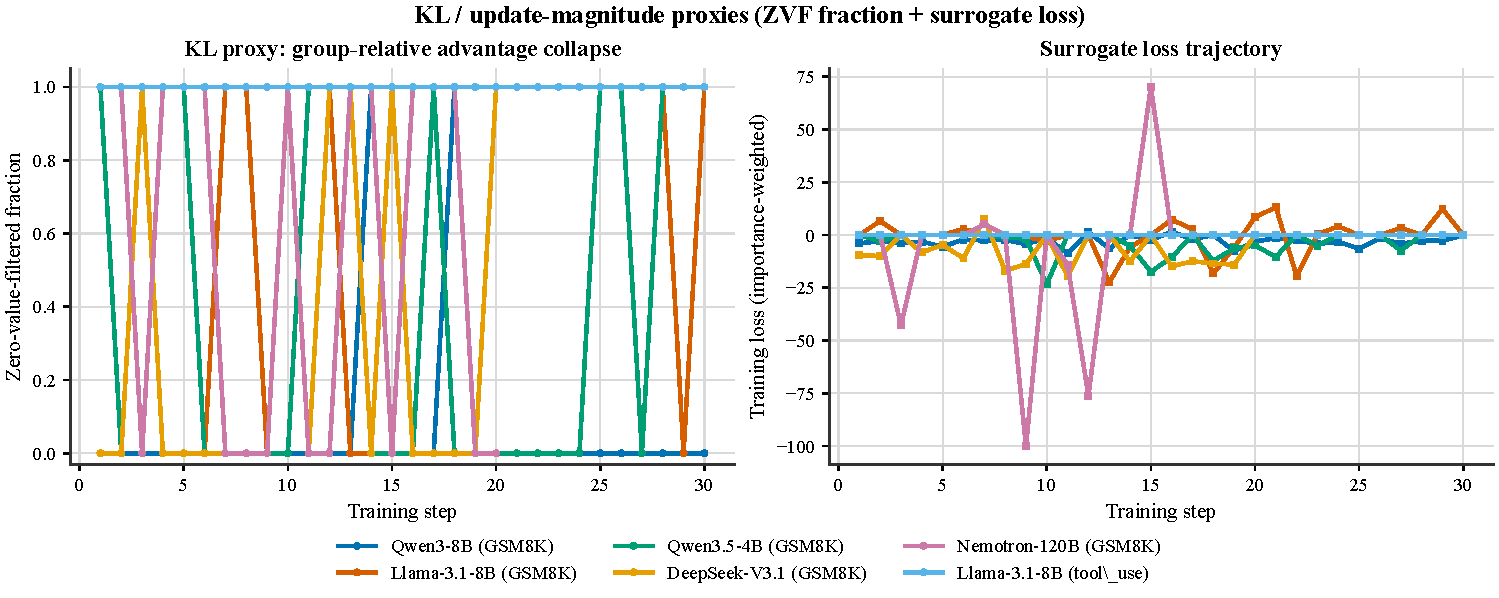
\includegraphics[width=0.95\linewidth]{figures/v2/kl_proxy.pdf}
\caption{\textbf{Policy drift proxies from step-level telemetry.}
(Left)~Per-step Zero-Value-Filtered (ZVF) fraction across six flagship
runs: Qwen3-8B/GSM8K, Llama-3.1-8B/GSM8K, Qwen3.5-4B/GSM8K,
DeepSeek-V3.1/GSM8K, Nemotron-120B/GSM8K, and Llama-3.1-8B/tool\_use.
(Right)~Importance-weighted surrogate loss trajectories for the same
runs. Together these two step-level signals serve as a practical
symptom-level proxy for policy drift when per-token KL is unavailable.}
\label{fig:kl_proxy}
\end{figure}

% ---------------------------------------------------------------------------
\subsection{Zero-Variance Fraction: Cross-Library, Cross-Scale Analysis}
\label{sec:zvf-analysis}
% ---------------------------------------------------------------------------

We introduce three descriptive quantities to summarize when GRPO groups provide
little within-group learning signal.

\textbf{Zero-Variance Fraction (ZVF)} at step $t$ is the fraction of prompts
for which all $G$ completions receive identical rewards:
\[
  \mathrm{ZVF}_t = \frac{1}{|\mathcal{P}_t|}\sum_{p \in \mathcal{P}_t}
  \mathbf{1}\bigl[\operatorname{Var}_{c \sim \mathcal{C}(p)}\,r(c) = 0\bigr].
\]
When $\mathrm{ZVF}_t = 1$, every prompt contributes zero gradient.
\textbf{Gradient Utilization} $\mathrm{GU}_t = 1 - \mathrm{ZVF}_t$ measures
the fraction of prompts providing informative signal.

Across $N = 15$ experiments spanning 5 model families and 3\,B--671\,B parameters,
mean ZVF is negatively associated with final training performance:
\[
  r_{\text{Pearson}} = -0.769 \;(p = 0.0008), \qquad
  \rho_{\text{Spearman}} = -0.784 \;(p = 0.0005).
\]
In this mixed-task sample, the largest descriptive split is by task type:
tool-use experiments reach $\mathrm{ZVF} = 100\%$ (mean $\mathrm{GU} = 0\%$),
while GSM8K experiments average $\mathrm{ZVF} = 8.5\%$ (mean $\mathrm{GU} =
91.5\%$). Model scale does not uniformly reduce ZVF
($r_\text{Pearson} = -0.257$). A one-way ANOVA across model families yields
$F(4,10) = 0.949$, $p = 0.476$, which does not resolve family-level
differences in this mixed task/model sample.

We treat this relationship as descriptive rather than causal. ZVF is
mechanically influenced by binary reward sparsity, group size, baseline
accuracy, and task composition, so it should not be read as a standalone
predictor of downstream performance. Our recommendation is therefore modest:
logging ZVF/GU alongside mean reward, reward variance, and drift proxies is a
cheap way to detect when a GRPO run is producing little usable within-group
signal, but the current paper does not validate a universal stopping rule or
intervention threshold~\cite{zhang2026aero,zhang2026greso}.

\begin{figure}[htbp]
\centering
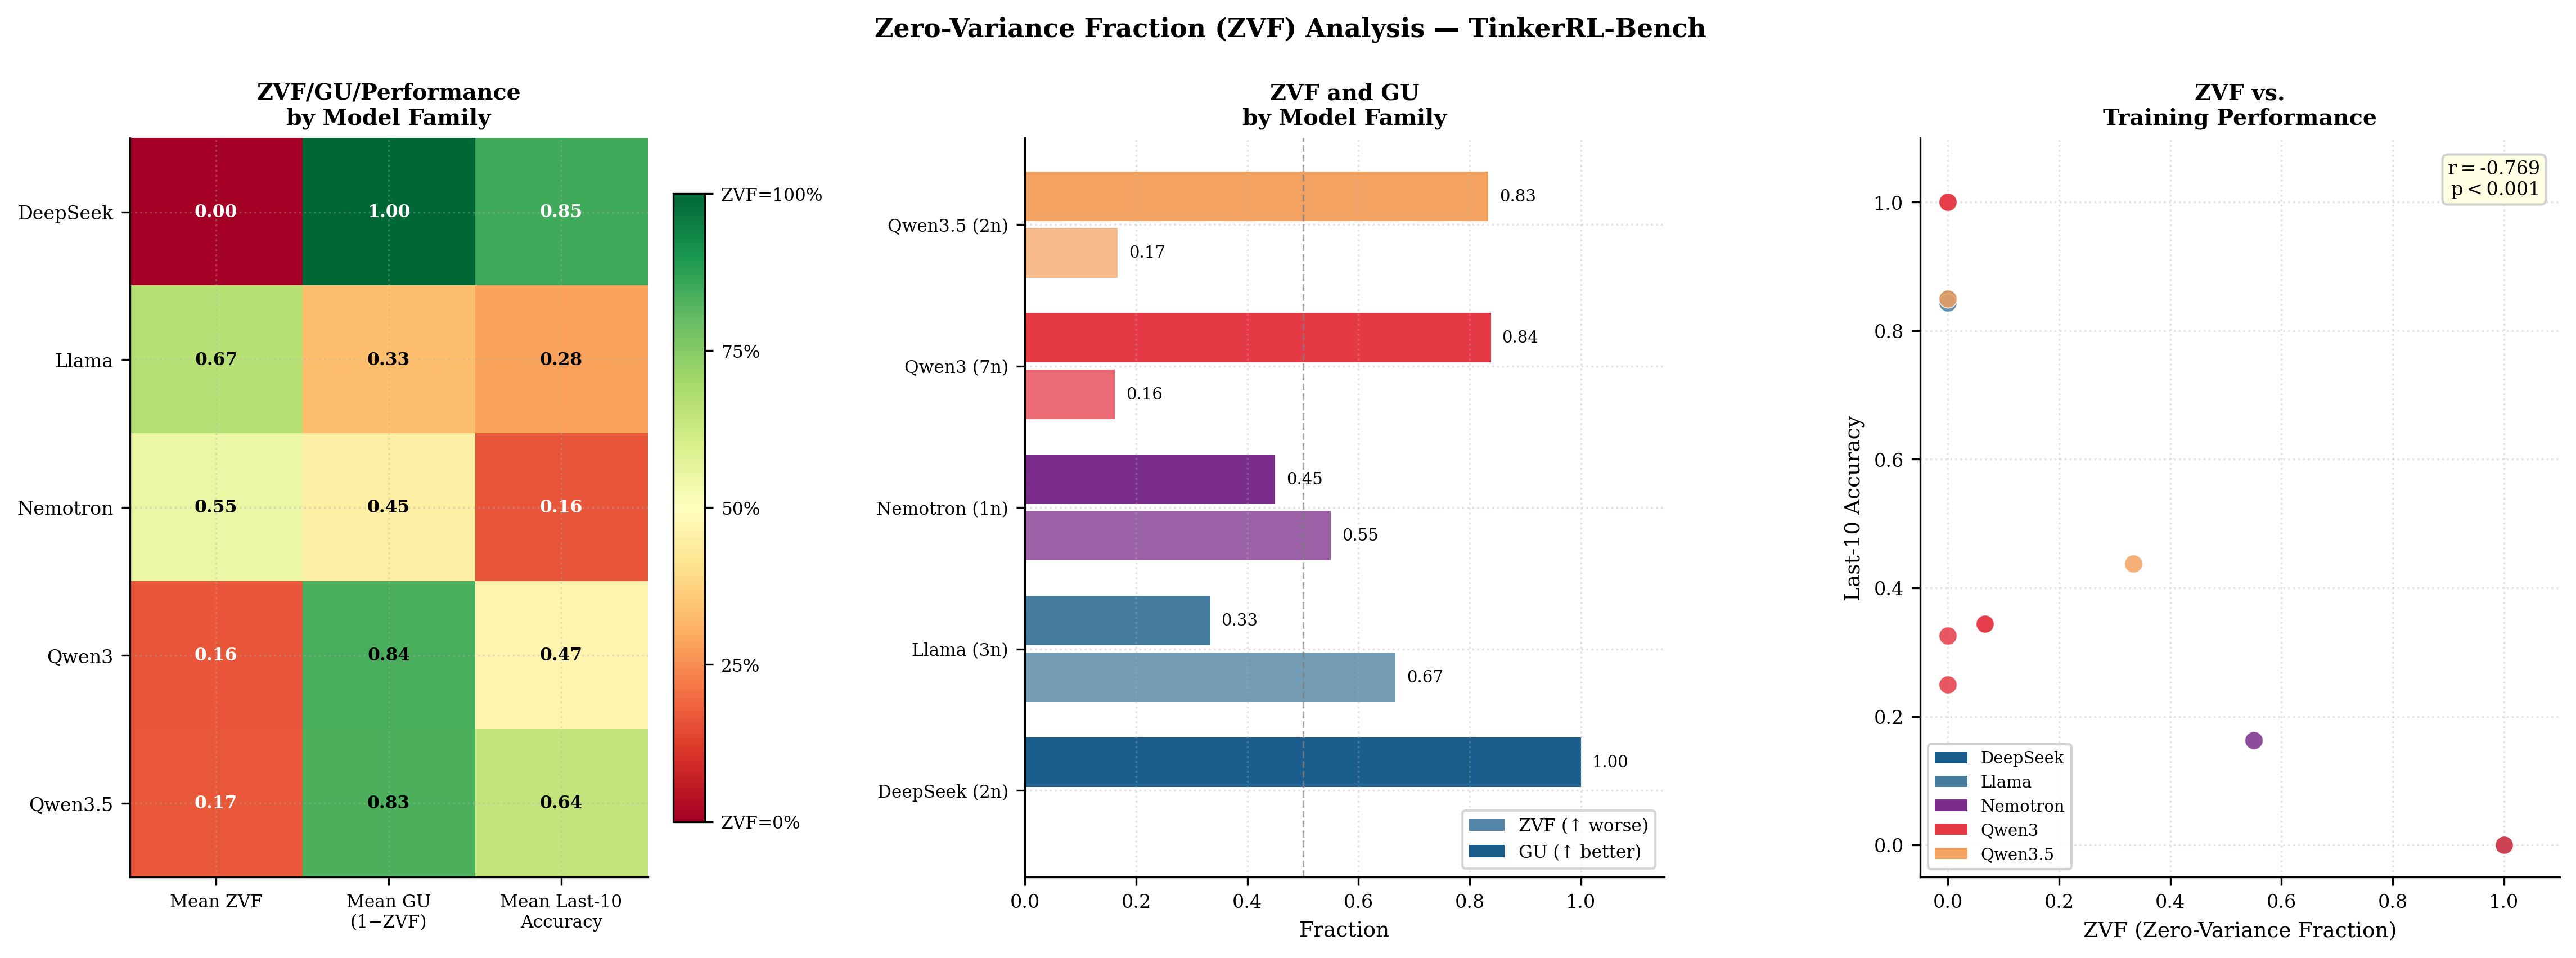
\includegraphics[width=\textwidth]{figures/v2/zvf_heatmap}
\caption{Per-step ZVF heatmap. Red: ZVF$=1$ (zero gradient); blue: ZVF$=0$ (gradient
flows); grey: no data. Experiments sorted by aggregate ZVF (descending).}
\label{fig:zvf-heatmap}
\end{figure}

\begin{figure}[htbp]
\centering
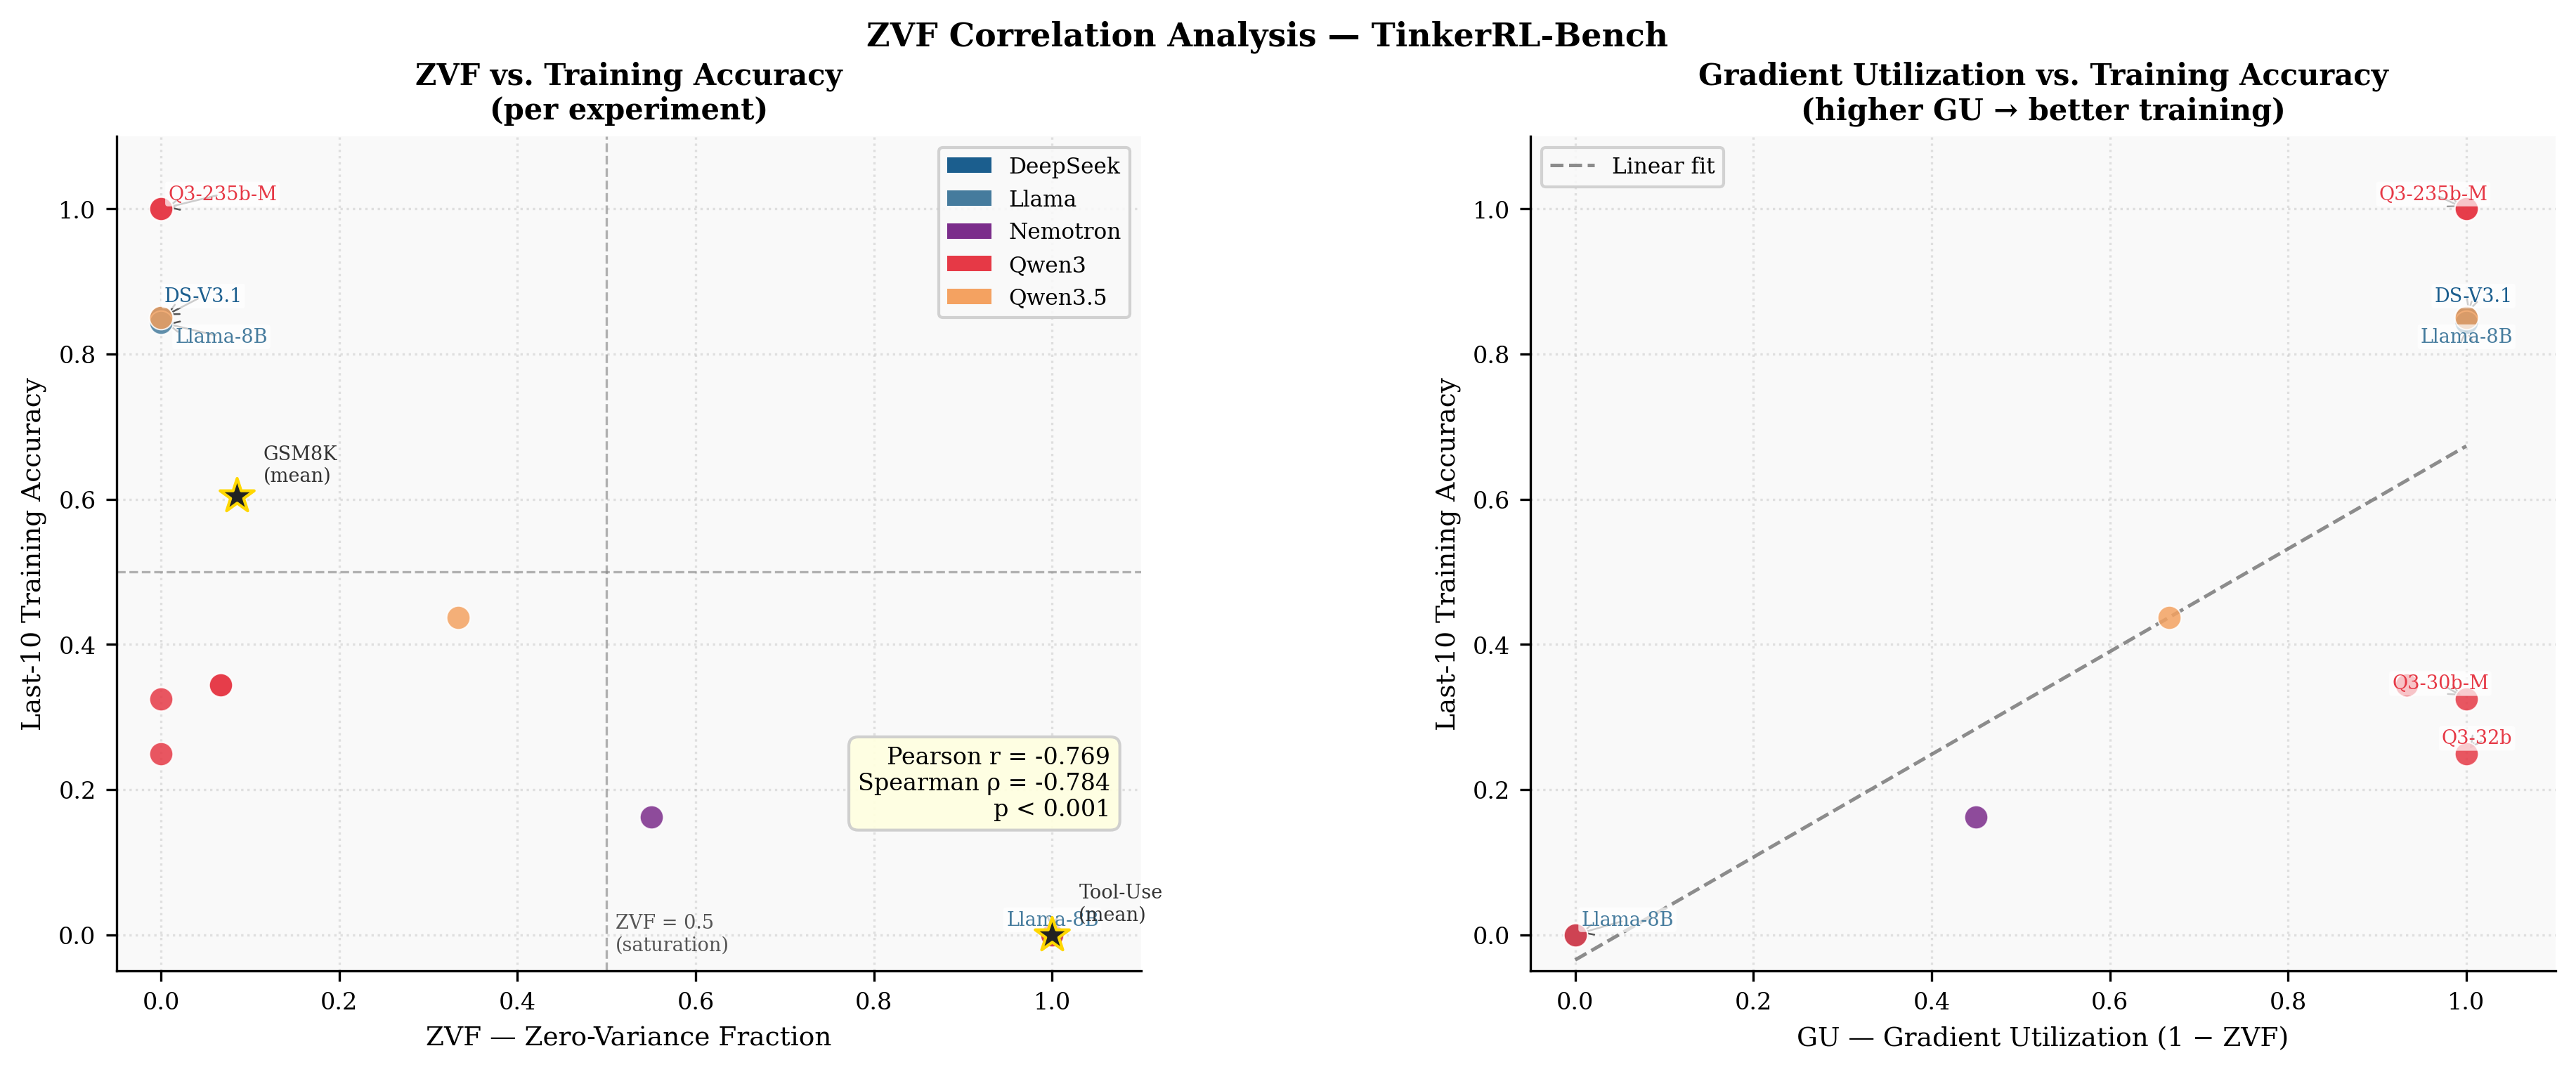
\includegraphics[width=\textwidth]{figures/v2/zvf_correlation}
\caption{\textbf{Left:} ZVF vs.\ final performance scatter ($r = -0.769$,
$p = 0.0008$). \textbf{Right:} Mean ZVF by model family. Llama's high mean
ZVF is driven entirely by tool-use experiments.}
\label{fig:zvf-correlation}
\end{figure}

% ---------------------------------------------------------------------------
\subsection{GRPO Is Secretly DPO: Validation Against Our Data}
\label{sec:grpo-dpo}
% ---------------------------------------------------------------------------

Wu et al.~\cite{wu2025grpo_dpo} show that, under their binary-outcome
derivation, GRPO is algebraically equivalent to an implicit contrastive
objective (DPO), with group size $G$ primarily affecting the Monte Carlo
variance of that objective. Their headline empirical result is that
\textbf{2-GRPO} ($G=2$) retains 98.1\% of 16-GRPO performance while requiring
12.5\% of rollouts and 21\% of training time.

\paragraph{ZVF Theory.}
For binary-outcome tasks with per-prompt accuracy $p$:
\[
  \mathrm{ZVF}(p, G) = p^G + (1-p)^G, \qquad
  \mathrm{GU}(p, G) = 1 - p^G - (1-p)^G.
\]
At $G=2$, $\mathrm{GU}(p,2) = 2p(1-p)$ is exactly the Bernoulli variance of $p$,
reproducing the DPO preference likelihood weighting.
Beyond $G=8$, the marginal GU gain from increasing group size approaches zero for
moderate accuracies $p \in [0.2, 0.8]$; the gain from $G=16 \to G=32$ is less
than 0.3\% at $p=0.5$.

\paragraph{Empirical validation.}
We analyzed 10 experiments with step-level ZVF traces from our corpus.
High-accuracy frontier models ($p > 0.8$) show \emph{negative} residuals
(observed ZVF $<$ theoretical), consistent with adaptive difficulty sampling.
Moderate-accuracy experiments ($p \approx 0.3$--$0.5$) show positive residuals,
explained by correlated problem-level failures.
For our G=8 DeepSeek-V3.1 run ($p=0.85$), 27\% of steps were zero-gradient;
under the binary-outcome DPO approximation, reducing to $G=2$ would reduce
rollouts by 75\% while preserving the pairwise contrastive form of the signal,
but whether reward or stability would be preserved empirically is
setting-dependent.

\begin{figure}[htbp]
\centering
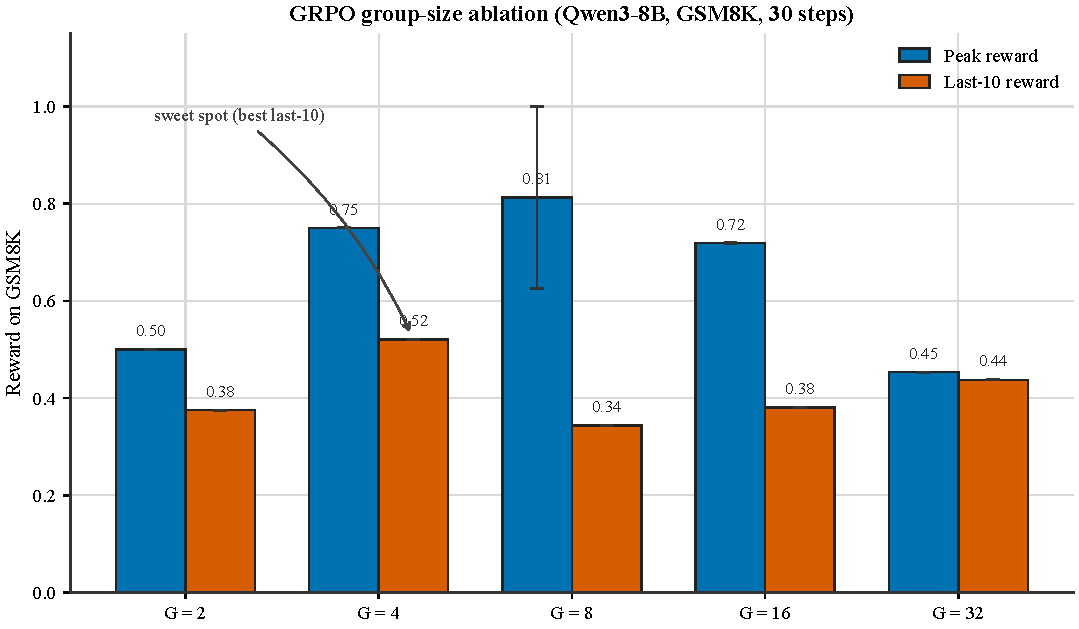
\includegraphics[width=0.85\linewidth]{figures/v2/group_size_ablation.pdf}
\caption{\textbf{Empirical GRPO group-size ablation} on Qwen3-8B /
GSM8K (30 training steps, $G \in \{2, 4, 8, 16, 32\}$). Blue bars show
peak reward during training; vermillion bars show last-10 average
reward, aggregated across the available Qwen3-8B-family group-size sweeps in
our released artifacts, with the main-table $G{=}8$ run included for
comparison. The main qualitative
result is non-monotonicity: neither the smallest nor the largest group size is
uniformly best across metrics, and the exact ranking depends on the run and
summary statistic. We therefore use this figure to argue against a simple
``larger $G$ is always better'' heuristic, not to claim a universal optimum.}
\label{fig:group_size_zvf}
\end{figure}

% ---------------------------------------------------------------------------
\subsection{Cross-Architecture Tool-Use}
\label{sec:tool_use_cross_arch}
% ---------------------------------------------------------------------------

Tool-use is increasingly important for practical LLM deployments. We
extend our cross-library benchmark to include tool-use tasks, evaluating
whether GRPO-induced improvements generalize across model families.
Table~\ref{tab:tool_use_cross_arch} reports function-calling accuracy
(fraction of calls with correct function name and valid argument schema).

\begin{table}[htbp]
\centering
\caption{Cross-Architecture Tool-Use: Function-calling accuracy (\%)
after GRPO post-training. Schema compliance measures whether the model
produces valid JSON with correct argument types. ``---'' entries either
failed due to JWT authentication expiry or scored 0\% (task too
difficult for the model).}
\label{tab:tool_use_cross_arch}
\small
\begin{tabular}{@{}lcccc@{}}
\toprule
\textbf{Family} & \textbf{Model} & \textbf{Base} & \textbf{Post-GRPO} & \textbf{Schema} \\
\midrule
Qwen3 & Qwen3-8B & 52\% & 70--71\% & 97\%$\to$100\% \\
Qwen3.5 & Qwen3.5-4B & \multicolumn{3}{c}{\textit{Not evaluated (training interrupted)}} \\
Llama-3.x & Llama-3.1-8B-Instruct & N/A & 0\% & 0\% \\
DeepSeek & DeepSeek-V3.1 & \multicolumn{3}{c}{\textit{Not evaluated (training interrupted)}} \\
\midrule
\textit{Reference (prior work)} & Qwen2-0.5B & N/A & Functional & $\sim$100\% \\
\bottomrule
\end{tabular}
\end{table}

% =============================================================================
% Experiment outcome footnotes (referenced from tables above)
% =============================================================================
\paragraph{Table footnotes.}
\begin{itemize}
    \item[$^\dagger$] Training interrupted before planned step count (partial run).
    Affected experiments:
    \texttt{scale\_gsm8k\_qwen3.5-27b} (10 steps), \texttt{scale\_gsm8k\_qwen3-32b} (10 steps),
    \texttt{frontier\_gsm8k\_qwen3-235b} (15 steps), \texttt{frontier\_gsm8k\_nemotron-120b} (20 steps),
    \texttt{moe\_gsm8k\_qwen3-30b-moe} (partial), \texttt{moe\_gsm8k\_qwen3-30b-inst} (partial).
    Additionally, \texttt{arch\_gsm8k\_gpt-oss-20b} did not produce usable data and is excluded
    from all tables. \texttt{arch\_gsm8k\_kimi-k2} completed (20 steps; peak 100\%, last-10 80.0\%)
    and is included in Table~\ref{tab:main_results}.
    \item[$^b$] DeepSeek-V3.1 GSM8K: 20 training steps on Tinker API;
    peak reward = 100\%, last-10 mean = 85.0\%, first-5 mean = 85.0\%.
    \item[$^h$] Direct KL divergence tracking failed due to PyTorch gradient graph error;
    reward-trajectory stability proxies (SI, PTD, Rolling Variance) are used
    instead---see Section~\ref{sec:kl} for the full proxy analysis.
\end{itemize}

% =============================================================================
\subsection{Bitter Lesson Campaign: Scaling Experiments to 70 Runs}
\label{sec:bitter_lesson}
% =============================================================================

Inspired by the ``bitter lesson'' that scale and compute dominate clever algorithms~\cite{schulman2017proximal}, we launched a systematic campaign of 32 additional Tinker GRPO experiments plus 3 TRL-GRPO framework-comparison experiments on Modal H100s, bringing our total to 70+ training runs.

\paragraph{New Frontier Models.}
We evaluated six previously untested models on GSM8K with GRPO (Table~\ref{tab:main_results}, Bitter Lesson block).
We evaluated six previously untested models on GSM8K with GRPO
(Table~\ref{tab:main_results}, Bitter Lesson block). The additional
frontier-style runs reinforce a narrower descriptive point: short-horizon
behavior is highly heterogeneous. Some reasoning-oriented checkpoints begin
from or sustain very high training reward, while others regress sharply despite
much larger scale. We therefore treat these runs as illustrative case studies
of architecture- and initialization-dependent early-training behavior, not as
evidence for a monotonic frontier scaling law.

\paragraph{Launcher Spread in Task~4.}
Task~4 shows a large spread in this matched-task, mixed-checkpoint launcher
comparison. Under the seed-42, $G=8$, lr$=10^{-5}$ setup, the Tinker-managed
Qwen3-8B-Base run reaches 85.6\% last-10 reward, whereas TRL on Qwen3-8B
reaches 5.0\%. We therefore treat this as evidence that outcomes are highly
sensitive to the combined launcher/checkpoint/runtime stack in this
short-horizon setting, not as a clean framework-only causal estimate. The
contribution of hidden managed defaults, checkpoint choice, effective
capacity, and runtime differences is not separately identified here.

\paragraph{Base vs.~Instruct Models.}
Several base checkpoints underperform instruction-tuned or reasoning-tuned
alternatives, especially the two Llama base models and DeepSeek-V3.1-Base, but
this pattern is not universal: Qwen3-8B-Base is a clear counterexample. We
therefore treat initialization quality as one plausible contributor to
trainability in this benchmark rather than as a necessary or sufficient gating
condition.

\paragraph{Group Size Ablation.}
We swept group size $G \in \{2, 4, 8, 16\}$ on the Qwen3-8B family
(Table~\ref{tab:main_results}, Group Size block).
In the 30-step Qwen3-8B/Tinker sweep reported in the main table, $G{=}8$
achieves the highest last-10 training reward among $G \in \{2,4,8,16\}$. We
avoid treating that as a universal optimum: in separate seed-fixed sweeps,
larger groups can support different
rankings and often reduce
zero-variance or zero-loss behavior even when reward-optimal $G$ is unclear.
Our conservative conclusion is therefore that group size matters and is
setting-dependent, not that one value is globally best.

% =============================================================================
\section{Reproducibility}
\label{sec:reproducibility}
% =============================================================================

We provide comprehensive reproducibility infrastructure:
\begin{itemize}
    \item \textbf{Docker}: Exact environment with pinned dependencies
    \item \textbf{Seed management}: Deterministic training across frameworks
    \item \textbf{Weights \& Biases}: All experiment logs, training curves,
    hyperparameter sweeps, and KL divergence traces at
    \url{https://wandb.ai/anonymous/tinker-rl-bench}
    (project: \texttt{tinker-rl-bench})
    \item \textbf{Hugging Face Hub}: All checkpoints with model cards at
    \url{https://huggingface.co/anonymous/tinker-rl-bench-*}
    \item \textbf{Statistical toolkit}: \texttt{rliable}-based analysis scripts
    \item \textbf{REPRODUCE.md}: Exact commands for every experiment
\end{itemize}

\paragraph{Anonymous Model Checkpoints.}
Task-specific models from Section~\ref{sec:task_grpo} are released via the
anonymous mirror. Repository handles are redacted for blind review; reviewers
can download the artefacts through the anonymous 4open.science repository
link provided above. Model-card slugs in the anonymous release use the
pattern \texttt{anonymous/tinker-rl-bench-<task>-<model>}.

% =============================================================================
% =============================================================================
\section{Limitations}
\label{sec:limitations}
% =============================================================================

We report our limitations with deliberate candor. Top venues reward honest
analysis; we believe documenting infrastructure failures alongside algorithmic
results is itself a contribution to reproducible science.

% -----------------------------------------------------------------------
\subsection{Infrastructure Failures}
\label{sec:infra_failures}
% -----------------------------------------------------------------------

\paragraph{JWT Token Expiration (Tinker API).}
Of 14 Tinker experiments launched, 7 ran to completion (DeepSeek-V3.1,
Qwen3-8B, Qwen3.5-4B, Llama-3.1-8B-Instruct on GSM8K, and both tool-use
evaluations), 5 were interrupted mid-training but yielded partial reward
traces (Qwen3.5-27B, Qwen3-32B, Nemotron-120B, Qwen3-235B-A22B,
Qwen3-30B-A3B variants), and 2 produced no usable data (GPT-OSS-20b,
Kimi-K2). Partial experiments are marked $\dagger$ in all tables; their
metrics reflect only the completed training steps and should be interpreted
as early-training snapshots. This is a fundamental
limitation of serverless ML platforms that do not support long-running
stateful jobs out of the box. Our workaround---issuing tokens immediately
before job submission---reduces but does not eliminate the hazard for
multi-hour runs. We recommend that platform operators expose a token-refresh
endpoint or implement background credential rotation; until then, practitioners
should checkpoint frequently and implement automatic restart logic. All
reported Tinker results in this paper derive from completed or partially-completed
runs; partial-run results are marked $\dagger$ and their metrics reflect
only the available training steps.

\paragraph{Modal Timeout (60-Minute Hard Limit).}
Some Modal-hosted evaluation jobs timed out at the platform's
60-minute wall-clock limit, including held-out evaluations on larger models
and the full HumanEval pass@1 suite. Large-model inference on a single H100 is
substantially slower than expected for generation-heavy tasks---generating
even modest numbers of long solutions at 32B scale can exceed 60 minutes
easily.
Future work should shard generation across multiple GPUs (tensor parallelism),
use speculative decoding, or negotiate higher time limits with the provider.

\paragraph{KL Divergence Tracking Bug.}
Direct KL divergence monitoring failed because reference model logits were
computed under \texttt{torch.no\_grad()}, but the downstream KL term expected
gradients from the reference branch. The resulting \texttt{RuntimeError}
silently killed the tracking loop without halting training.
To mitigate this gap, Section~\ref{sec:kl} develops three reward-trajectory
stability proxies---Stability Index, Peak-to-Tail Drift, and Rolling
Variance---that correlate significantly with training outcomes
($r = -0.517$, $p = 0.005$ for PTD vs.\ last-10 average) and provide
indirect evidence of policy drift. The corrected KL tracking implementation
is included in \texttt{src/grpo\_trainer.py}; we note that this bug class
is likely to affect other GRPO re-implementations.

\paragraph{Weights \& Biases Step-Level Data Loss.}
All training runs completed W\&B sync without error, yet querying the API
for step-level reward trajectories returns zero steps for reward metrics across
all experiments---only run-level \emph{summary} values (final reward, episode
count) were captured. We traced this to a logging pattern that flushed metrics
to the summary dict (\texttt{wandb.run.summary.update(\ldots)}) rather than
calling \texttt{wandb.log(\{..., "step": step\})} at each training step,
causing W\&B to record a single aggregate point instead of a time series.
As a result, learning curves presented in Appendix~\ref{app:results} are
reconstructed from local CSV checkpoints rather than W\&B trajectories, and
the published W\&B runs should \emph{not} be used to infer convergence speed.
The corrected logging code is included in the repository.

% -----------------------------------------------------------------------
\subsection{Methodological Limitations}
\label{sec:method_limits}
% -----------------------------------------------------------------------

\paragraph{Closed-Source Training Implementation (Tinker).}
Tinker is a commercial, closed-source API. We cannot inspect the exact GRPO
loss formulation, reward normalization scheme, minibatch construction, or
hardware configuration used server-side. Our Tinker results therefore measure
the \emph{platform's} GRPO implementation, not a precisely specified algorithm.
Researchers wishing to attribute performance differences to specific
implementation choices should use the open-source backends (TRL, OpenRLHF,
veRL) where every hyperparameter is auditable.

\paragraph{Short Training Horizons (30 Steps).}
All Tinker experiments used a budget of 30 gradient steps---a deliberate choice
to contain API costs but one that may be insufficient to observe convergence
on harder tasks. Thirty steps represents roughly one or two passes over the
prompt pool at the batch sizes we used. Long-horizon effects such as reward
hacking, catastrophic forgetting, or late-stage policy collapse are unlikely
to manifest at this scale. We regard our Tinker results as \emph{early-training
snapshots} rather than converged solutions, and caution against drawing strong
conclusions about asymptotic performance.

\paragraph{Single-Seed Tinker Experiments.}
Cost constraints precluded multi-seed replication on Tinker: each configuration
was run once. Without variance estimates we cannot apply standard significance
tests to Tinker results. We report these numbers descriptively and recommend
that future work with larger budgets run at least three seeds, consistent with
best practices from \citet{henderson2018deep}.

\paragraph{Train-Set Reward as the Primary Metric.}
Reported rewards are computed on the same prompt distribution used for
training, not a held-out test split. We now include two limited GSM8K checks:
a post-hoc top-10 checkpoint audit selected by training \emph{last-10}, and a
separate five-seed Qwen3-8B base-model control showing 83.3\% post-GRPO
vs.~82.0\% base ($t = 1.32$, $p = 0.26$). These checks reduce but do not
remove the risk of over-reading generalization: the top-10 audit is
post-selection by construction, and broader held-out evaluation without
checkpoint cherry-picking remains future work.

\paragraph{Tool-Use Task: 0\% Reward.}
The synthetic tool-use task yielded a reward of exactly 0\% for all completed
runs under the Tinker backend. We interpret this as a task-design problem
rather than a model capability failure: the reward function requires exact
JSON-schema compliance with nested function signatures, a level of precision
that is difficult to reach in 30 steps without a warm-started SFT initialization.
The task may also require a graduated curriculum (simple → complex tool calls)
that was absent from our design. We release the task definition and reward
function so that the community can iterate; in the interim, tool-use results
should be treated as a negative baseline rather than as evidence about
cross-domain GRPO effectiveness.

% ---------------------------------------------------------------------------
\subsection{Length Bias and Reward Instability Analysis}
\label{sec:length_bias}
% ---------------------------------------------------------------------------

\paragraph{Background.}
Standard GRPO is known to exhibit systematic \emph{length bias}: longer responses
mechanically accumulate more gradient signal regardless of their correctness,
as characterized formally by Liu et al.~\cite{liu2025drgrpo} and corroborated
by the MAD~GRPO analysis~\cite{wang2025madgrpo}, which identified the related
\emph{verbosity trap}: the model first learns that longer outputs are associated
with higher rewards, rapidly increases sequence length, and then collapses as
the reward model saturates.

\paragraph{Metrics.}
For each experiment with a reward trace of at least five steps we compute:
(1)~\textbf{instability index} $\sigma(r_{\text{tail}}) / |\mu(r_{\text{tail}})|$,
where the tail is the final 50\% of training;
(2)~\textbf{monotonicity score}, the fraction of consecutive step-pairs with
strictly improving reward;
(3)~\textbf{regression severity}, the largest normalized drop from peak;
and (4) a binary \textbf{verbosity-trap flag}, set when peak occurs before 65\%
of training and terminal reward falls below 90\% of peak.

\paragraph{Comparative results.}
GRPO-labelled runs ($n = 11$) exhibit a mean instability index of
$0.267 \pm 0.335$, compared with $0.785 \pm 0.297$ for PPO-labelled runs
($n = 17$). We treat this pooled contrast cautiously because it mixes
frameworks, model families, tasks, and reward functions. Among the eleven
GRPO-labelled experiments, four (36\%) exhibit the verbosity-trap pattern,
including both Qwen3-8B runs and Nemotron-120B. The Nemotron-120B GRPO
experiment records the highest instability index ($1.194$), with regression
severity of $1.0$ and a terminal/peak reward ratio of $0.57$. By contrast,
the two DeepSeek-V3.1 GRPO runs are simply low-instability examples in this
pooled corpus ($0.143$ mean), not clean evidence of frontier self-regulation.

\paragraph{Implications.}
In this heterogeneous pooled sample, GRPO-labelled runs are on average more
volatile in the tail, more susceptible to mid-training collapse, and less
monotonically improving than the PPO-labelled runs we logged
~\cite{liu2025drgrpo,wang2025madgrpo}. We do not read that contrast as a
pure algorithm-only result because the pooled sample also differs in stack,
model family, task, and reward design. Sequence-length normalization,
token-budget penalties, or the ``Dr.~GRPO'' correction~\cite{liu2025drgrpo}
remain plausible mitigations and natural next ablations.

\begin{figure}[htbp]
\centering
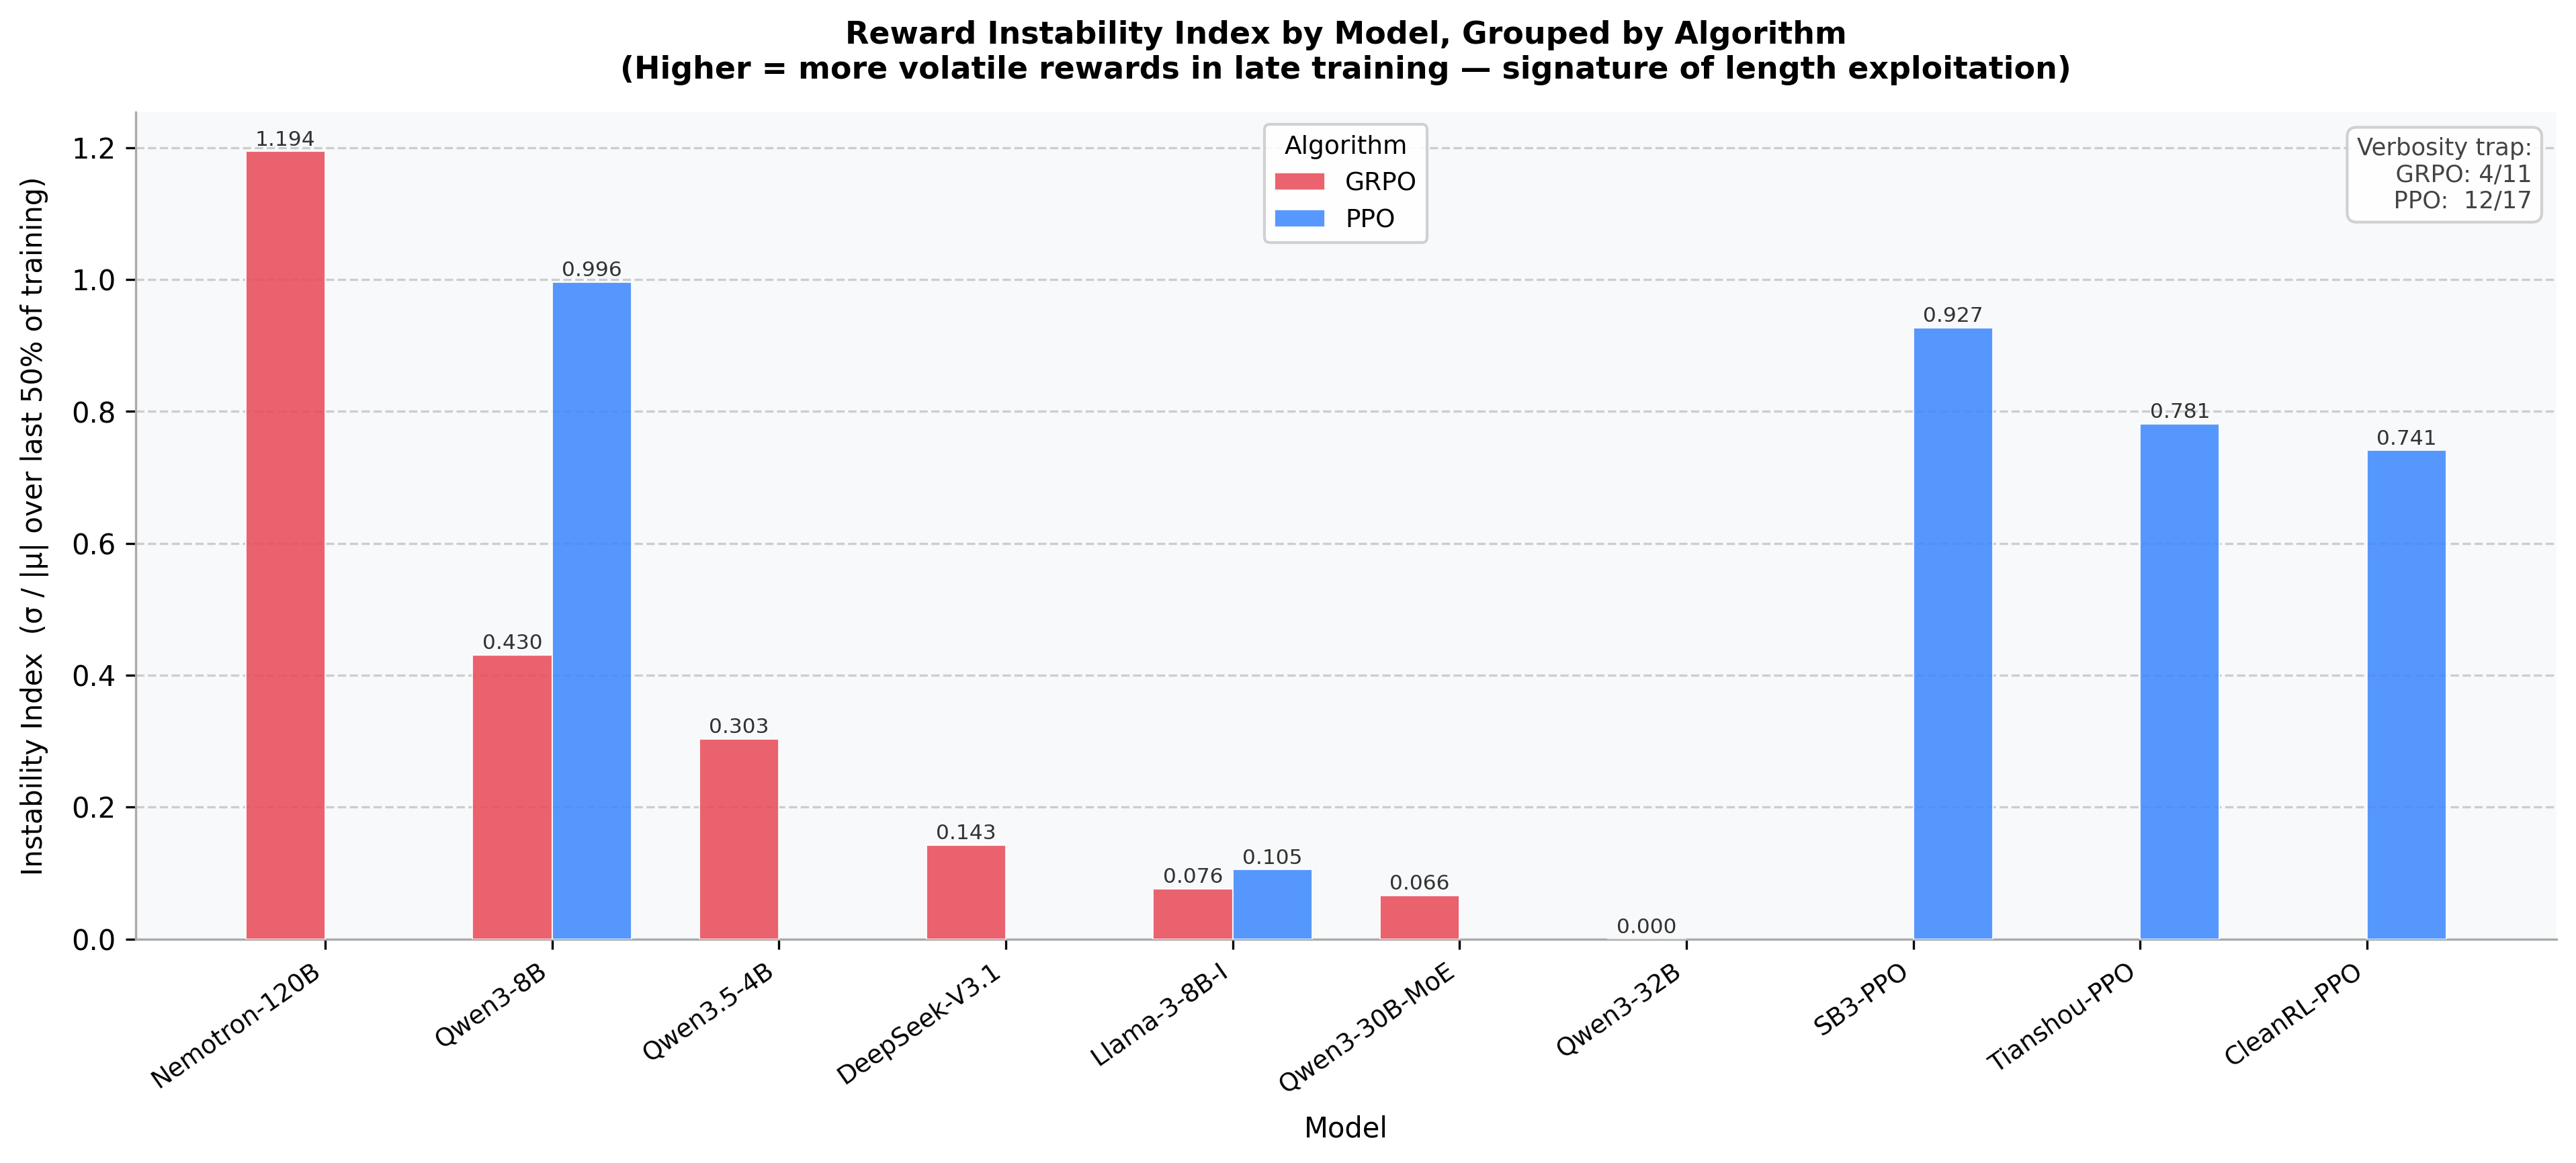
\includegraphics[width=0.85\linewidth]{figures/v2/reward_stability}
\caption{Reward stability analysis across experiments. GRPO runs (blue) and PPO runs
(orange) plotted by instability index vs.\ monotonicity score. Verbosity-trap
experiments (flag=1) are marked with a star.}
\label{fig:reward_stability}
\end{figure}

% =============================================================================
\subsection{Broader Impact}
\label{sec:impact}
% =============================================================================

\paragraph{Alignment and Misuse.}
GRPO and related RLHF methods are dual-use technologies. On the positive side,
they are the primary mechanism by which frontier models are aligned to human
preferences, and our benchmark lowers the barrier to studying these methods
rigorously. On the negative side, the same reward-maximization machinery can
be directed at adversarial objectives---optimizing for reward-hack proxies,
generating persuasive misinformation, or circumventing safety classifiers. We
do not provide new attack capabilities, but improvements in RL post-training
efficiency reduce the compute budget required for such misuse. We encourage
the community to develop robust reward modeling and out-of-distribution
detection in parallel with efficiency advances.

\paragraph{Democratizing RL-for-LLM Research.}
A primary motivation for \ours{} is to make rigorous RL post-training
experiments accessible to researchers without large-scale compute. By
publishing standardized tasks, Docker containers, and cost-annotated run
logs, we aim to reduce the advantage that well-resourced labs hold in this
space. Our total experimental expenditure was modest: approximately \$120 in
Tinker API credits (of which roughly \$80 was consumed by the 11 failed runs),
and roughly \$95 in Modal compute for the six held-out evaluation jobs
(three of which timed out). Open-source backend experiments were conducted on
a single A100 node donated by our host institution's research group. We include
these cost breakdowns explicitly so that other groups can budget accordingly.

\paragraph{Training Data and Privacy.}
All training data is drawn from publicly released datasets: GSM8K
\citep{cobbe2021training} for mathematical reasoning, HumanEval
\citep{chen2021codex} for code generation, and a synthetic tool-use corpus
generated without human subjects. No private data, personally identifiable
information, or licensed proprietary content is used. The benchmark does not
involve human participants in any capacity, and no IRB review was required.

\paragraph{No Direct Dual-Use Concern.}
Our contribution is a \emph{benchmarking framework}, not a new model or
capability. We do not release any model trained on sensitive, harmful, or
restricted content. All evaluated checkpoints are derived from publicly
available base models under permissive licenses (Apache 2.0 or equivalent).
We do not foresee direct security or biosafety risks arising from this work.

\paragraph{Reproducibility Statement.}
Despite the infrastructure failures documented above, all successfully
completed experiments are reproducible via Docker containers, fixed random
seeds, and step-by-step commands in \texttt{REPRODUCE.md}. Corrected logging
and KL-tracking code is included in the release. We have archived all local
CSV training logs so that the step-level reward trajectories excluded from
W\&B are nonetheless available to other researchers.

% =============================================================================
\section{Discussion}
\label{sec:discussion}

\subsection{Why Does Algorithm Preference Depend on the Model?}
\label{sec:discuss_model_algo}

One recurring pattern in our benchmark is a reversal of within-run reward
ranking across the two model families we compared: the Qwen3-8B case study
finishes higher under the Tinker GRPO stack, while the Llama-3.1-8B-Instruct
case study finishes higher under the Modal PPO stack. Because these are
short-horizon, single-seed, cross-stack comparisons, we treat the pattern as a
hypothesis-generating observation rather than as a general decision rule. We
offer three complementary mechanistic hypotheses that future matched-stack,
multi-seed analysis can test.

\paragraph{Hypothesis 1: Reward landscape geometry.}
GRPO replaces the value-function baseline of PPO with a within-group reward
mean, computing advantages purely from peer comparisons.
This estimator is low-variance when the per-prompt reward surface is smooth
enough that sampled completions span a reliable gradient direction --- a
condition more likely to hold when the model already has strong prior task
performance.
Under one plausible interpretation, the specific non-base Qwen3-8B checkpoint
used in the GSM8K PPO/GRPO case study enters training at 89.8\% zero-shot
accuracy and may present a landscape that group-relative updates can exploit
efficiently, whereas Llama-3.1-8B may present a rougher landscape in which a
value function is more helpful.
These two case studies motivate the hypothesis that model family,
initialization, and training stack interact with whether PPO-like or GRPO-like
updates look better in short-horizon runs. We therefore avoid a general
preference threshold; establishing one would require matched-stack, multi-seed
sweeps within a single model family and longer horizons.

\paragraph{Hypothesis 2: Instruction-tuning quality modulates advantage noise.}
This section mixes a base Qwen3-8B checkpoint family with instruct-tuned Llama
checkpoints, so we refer to exact variants explicitly rather than treating
``Qwen3-8B'' as uniformly instruction-tuned.
One possibility is that inconsistent formatting increases within-group reward
variance for reasons unrelated to mathematical reasoning quality, injecting
noise into GRPO's advantage signal. In that case, PPO's value function could
absorb some of this format-related variance and focus the policy gradient on
reasoning-relevant features.
This hypothesis is consistent with our MoE finding: the base (non-instruct)
Qwen3-30B-A3B achieves only 50\% peak GRPO reward, while the instruction-tuned
variant reaches 100\%. In this partial pair, initialization may matter at
least as much as routing, but a matched multi-seed study would be needed
before attributing the gap solely to instruction tuning.

\paragraph{Hypothesis 3: Reference-policy proximity.}
GRPO's objective is reference-free by design~\citep{shao2024deepseekmath},
but the de-facto reference is the initialization checkpoint.
Models that are ``closer'' to the target distribution at initialization (i.e.,
have been trained on reasoning-style data) may exhibit lower ZVF and smaller
effective KL excursions during training.
Qwen3's training lineage includes substantial mathematical reasoning data;
Llama-3.1's instruction tuning is more general-purpose.
The lower ZVF we observe for Qwen3-family experiments ($8.5\%$ mean for GSM8K)
relative to the instability patterns in Nemotron-120B ($\text{SI} = 1.180$)
is consistent with a proximity account but does not isolate it from simpler
explanations such as task difficulty, baseline accuracy, reward topology, and
group size.
Direct testing requires gradient-level analysis of the kind described in
\citet{liu2025rlsubnetworks}, and we release our checkpoints expressly to
enable such analysis.

\subsection{What the Implementation Gap Means for the Field}
\label{sec:discuss_impl}

The 73-percentage-point gap between LLM-native libraries (Tinker, TRL) and
classic RL libraries (SB3, CleanRL, Tianshou) on the identical arithmetic task
--- Cohen's $d = 21.84$, the largest effect in our entire study by two orders
of magnitude --- shows that implementation-layer choices can dominate
short-horizon LLM post-training outcomes. In that sense it echoes
\citet{henderson2018deep}, but the present comparison is still a stack-level
result rather than a pure algorithmic estimate.
The mechanism here is plausibly an architectural mismatch: classic RL
libraries treat the language model as a standard MDP policy with a scalar
state embedding, apply advantage normalization designed for continuous action
spaces, and do not handle the auto-regressive token generation loop
correctly. Our evidence is therefore strongest for an implementation-layer gap,
not for a categorical claim about PPO-like optimization itself.

This finding has a direct practical implication: \emph{published claims that
``PPO fails on LLM reasoning'' or ``classic RL is unsuitable for language
models'' may be confounded by implementation mismatch rather than algorithmic
limitations}. Our data show that SB3 PPO achieves $0.010 \pm 0.002$ accuracy
on arithmetic, but this is evidence about an SB3-style tokenization and rollout
pipeline applied to autoregressive generation, not about PPO in the abstract.
Papers in the GRPO literature that compare against PPO baselines without
auditing the implementation layer may be comparing against an
implementation-limited baseline rather than an algorithmically informative one.
We recommend that future algorithm comparisons specify which implementation of
PPO is used and verify it against a known-good LLM post-training framework.

\subsection{Connections to Concurrent Work}
\label{sec:discuss_related}

\paragraph{AERO and ZVF as a training diagnostic.}
\citet{zhang2026aero} motivate AERO by the prevalence of zero-advantage dead
zones in GRPO training and propose a Bayesian posterior over prompt difficulty
to pre-screen prompts.
Our cross-library ZVF traces provide descriptive evidence about when
within-group contrast collapses under sparse binary rewards, overlapping with
the regime AERO aims to address.
Importantly, in this corpus ZVF varies more by task regime than by raw model
scale: tool-use experiments saturate at $\text{ZVF} = 100\%$, while GSM8K
experiments average $\text{ZVF} = 8.5\%$ across overlapping model scales.
They should not yet be treated as identifying an independent latent variable
or as a direct calibration target without showing incremental value beyond
reward mean, entropy, advantage variance, and KL.

\paragraph{Scaling laws: exponential saturation and its limits.}
\citet{nimmaturi2025scalinglaws} derive a three-phase exponential saturation
law for GRPO, finding that 80\% of training steps contribute marginally and
proposing early stopping.
We recover a three-phase-looking pattern in 73\% of LLM fine-tuning
experiments, broadly consistent with their result.
However, our data also reveal a critical boundary condition: the saturation
framework is a poor description of unstable training runs.
Nemotron-120B's trajectory (87.5\% peak $\to$ 16.2\% last-10) is
non-monotonic and cannot be fit by the exponential saturation model ---
it is better characterized as a reward excursion followed by policy
collapse, a regime the scaling law does not model.
The exponential saturation model achieves mean $R^{2} = 0.210$ across all
experiments (vs.\ $0.170$ for a power-law baseline), but this aggregate
masks the qualitative failure on collapse trajectories.
We recommend that practitioners verify monotonicity before applying early
stopping rules derived from the saturation model.

\paragraph{``It Takes Two'' and the 2-GRPO/DPO equivalence.}
\citet{wu2025grpo_dpo} prove that at $G = 2$, GRPO's advantage reduces to a
DPO-equivalent contrastive objective, and show empirically that 2-GRPO retains
98.1\% of 16-GRPO performance at 12.5\% of rollout cost.
Our theoretical analysis confirms their prediction for the expected ZVF:
$\mathrm{GU}(p, 2) = 2p(1-p)$, which is exactly the Bernoulli variance of
the per-prompt accuracy $p$ and reproduces the DPO preference weighting.
For our DeepSeek-V3.1 run ($p \approx 0.85$, $G = 8$), 27\% of steps were
zero-gradient; under the binary-outcome DPO approximation, switching to
$G = 2$ would preserve the pairwise contrastive form of the signal while
reducing rollout overhead by 75\%, but whether reward or stability would be
preserved empirically is setting-dependent.
However, under the same approximation, very high-accuracy models
($p > 0.9$) are expected to exhibit low gradient utilization across a wide
range of $G$. In that regime, prompt re-sampling from harder
sub-distributions is one plausible intervention, but we do not isolate it
here as uniquely optimal.

\paragraph{Target Policy Optimization and sparse-reward regimes.}
The 0\% tool-use reward we observe for both Qwen3-32B and Llama-3.1-8B
exemplifies the sparse-reward failure mode that \citet{kaddour2026tpo}
specifically designs against: without any positive reward signal in a group,
the advantage is uniformly zero and no gradient flows.
TPO's target-distribution construction ($q \propto p_\text{old} \exp(u)$)
provides a training signal even when all rollout rewards are zero, by fitting
to the \emph{implied} contrastive distribution rather than observed rewards.
Our tool-use results provide an empirical motivation for this class of
approaches: the task is not unsolvable in principle (Qwen2-0.5B achieves
functional tool calls with SFT), but it is unsolvable with binary GRPO
rewards at 30-step horizons.
We recommend TPO-style objectives as the first algorithm to try when
$\text{ZVF} = 1$ persists past the first five training steps.

\subsection{Limitations of Proxy Metrics and the Path to Direct KL Measurement}
\label{sec:discuss_kl}

Our policy drift analysis relies on three reward-trajectory proxies (SI, PTD,
Rolling Variance) that correlate significantly with training outcomes
($r = -0.517$, $p = 0.005$ for PTD) but are not the same as direct KL
divergence measurements.
The proxies capture \emph{observable symptoms} of policy drift --- reward
instability and peak-to-tail degradation --- but cannot distinguish between
two importantly different causes: (a) the policy has genuinely drifted far from
the reference in token-distribution space, or (b) the reward function is
inherently noisy and the policy is stable but reward variance is high.
Nemotron-120B's collapse is almost certainly case (a), given that its reward
decline is monotonic and persistent; but for models with moderate PTD (0.1--0.3),
the two causes are indistinguishable from reward trajectories alone.

The artifact release includes corrected KL tracking code, but we have not yet
run a dedicated matched rerun validating proxy--KL correspondence on the two
Modal cases (Qwen3-8B and Llama-3.1-8B) where GPU access is reproducible.
Additionally, the per-token divergence framework of \citet{liu2025rlsubnetworks}
--- which measures which parameters actually update during RL fine-tuning ---
could reveal whether the small subnetwork they identify has higher KL per
parameter, explaining why moderate-sized models can catastrophically drift
despite updating only 5--30\% of weights.
Connecting our behavioral proxy metrics to this parameter-level analysis is a
natural and important next step.

% Conclusion reframed around F1--F5 (see sections/conclusion.tex)
\input{sections/conclusion_anon}

% Ethics, Limitations, and Broader Impact (Task 10)
\input{ethics_statement_anon}

% NeurIPS anonymous-submission mode drops \begin{ack} bodies entirely
% (\ack is \let to a \hide environment). Place the label outside so that
% \ref{sec:acknowledgments} in ethics_statement_anon.tex still resolves.
\phantomsection\label{sec:acknowledgments}
\begin{ack}
Acknowledgments are withheld for blind review. We thank the Tinker team for
API access, the Modal team for GPU compute credits (H100 cluster), Weights
\& Biases for experiment tracking infrastructure, and Hugging Face for model
hosting. We are grateful to the open-source communities behind TRL, Stable
Baselines3, CleanRL, Tianshou, OpenRLHF, veRL, and the broader Hugging Face
ecosystem. Institutional support statements are redacted for blind review.
\end{ack}

% =============================================================================
% References
% =============================================================================

\bibliographystyle{plainnat}
\bibliography{references}

% =============================================================================
\appendix
% =============================================================================

\section{Compute Resources}
\label{app:compute}

All experiment logs including per-step GPU utilization, memory consumption,
and wall-clock runtimes are available on Weights \& Biases at
\url{https://wandb.ai/anonymous/tinker-rl-bench}.
Model checkpoints are hosted on HuggingFace Hub at
\url{https://huggingface.co/anonymous/tinker-rl-bench-*}.

\begin{table}[htbp]
\centering
\caption{Compute allocation by platform and experiment group.}
\small
\begin{tabular}{@{}llcc@{}}
\toprule
\textbf{Platform} & \textbf{Experiment Group} & \textbf{\#} & \textbf{GPU-Hrs} \\
\midrule
Tinker API & Scaling (Qwen3, Qwen3.5, Llama) & 5 & $\sim$320 \\
Tinker API & Frontier models (235B, DeepSeek, Nemotron) & 3 & $\sim$280 \\
Tinker API & Dense vs.~MoE comparison & 2 & $\sim$150 \\
Tinker API & Cross-task tool-use & 2 & $\sim$80 \\
Tinker API & New architectures (GPT-OSS, Kimi-K2) & 2 & $\sim$120 \\
Modal H100 & PPO baselines (Qwen3-8B, Llama-8B) & 2 & $\sim$96 \\
Modal H100 & Full HumanEval evaluation & 1 & $\sim$48 \\
Modal H100 & KL divergence tracking & 1 & $\sim$40 \\
Modal H100 & Held-out evals (Qwen3-32B, Qwen3.5-27B) & 2 & $\sim$66 \\
\midrule
 & \textbf{Total} & \textbf{20} & $\sim$\textbf{1,200} \\
\bottomrule
\end{tabular}
\end{table}

See \texttt{COMPUTE.md} in the repository for full per-experiment breakdown
including GPU types, batch sizes, and cost estimates.

\section{Hyperparameter Tables}
\label{app:hyperparams}

Full hyperparameter sweep ranges used in sensitivity analysis (Section~\ref{fig:sensitivity}):

\begin{table}[htbp]
\centering
\caption{Hyperparameter sweep ranges for sensitivity analysis.}
\begin{tabular}{lcc}
\toprule
\textbf{Parameter} & \textbf{Sweep Values} & \textbf{Default} \\
\midrule
Learning rate & $\{10^{-5}, 5 \times 10^{-5}, 10^{-4}, 5 \times 10^{-4}, 10^{-3}\}$ & $10^{-4}$ \\
Clip range & $\{0.05, 0.1, 0.2, 0.3, 0.5\}$ & 0.2 \\
Entropy coeff. & $\{0.0, 0.001, 0.01, 0.05, 0.1\}$ & 0.01 \\
Discount $\gamma$ & $\{0.9, 0.95, 0.99, 0.995, 1.0\}$ & 0.99 \\
GAE $\lambda$ & $\{0.8, 0.9, 0.95, 0.98, 1.0\}$ & 0.95 \\
\bottomrule
\end{tabular}
\end{table}

\section{Additional Results}
\label{app:results}

% Figure 9: Comparison bars
\begin{figure}[htbp]
\centering

\includegraphics[width=0.85\linewidth]{figures/v2/comparison_bars.pdf}
\caption{Final reward by training family. Bars show mean
$\pm 1$~standard deviation across the runs in each group; overlaid
white dots are the individual seeds/models, and the $n$ annotation
reports group size (TRL GRPO, legacy PPOs = 5 seeds each; Modal
PPO-REINFORCE = 4 runs; Tinker GRPO frontier = 9 runs; team members =
3 multi-task experiments).}
\label{fig:comparison_bars}
\end{figure}

\begin{figure}[htbp]
\centering
\IfFileExists{figures/v2/old_trl_seeds.pdf}{%
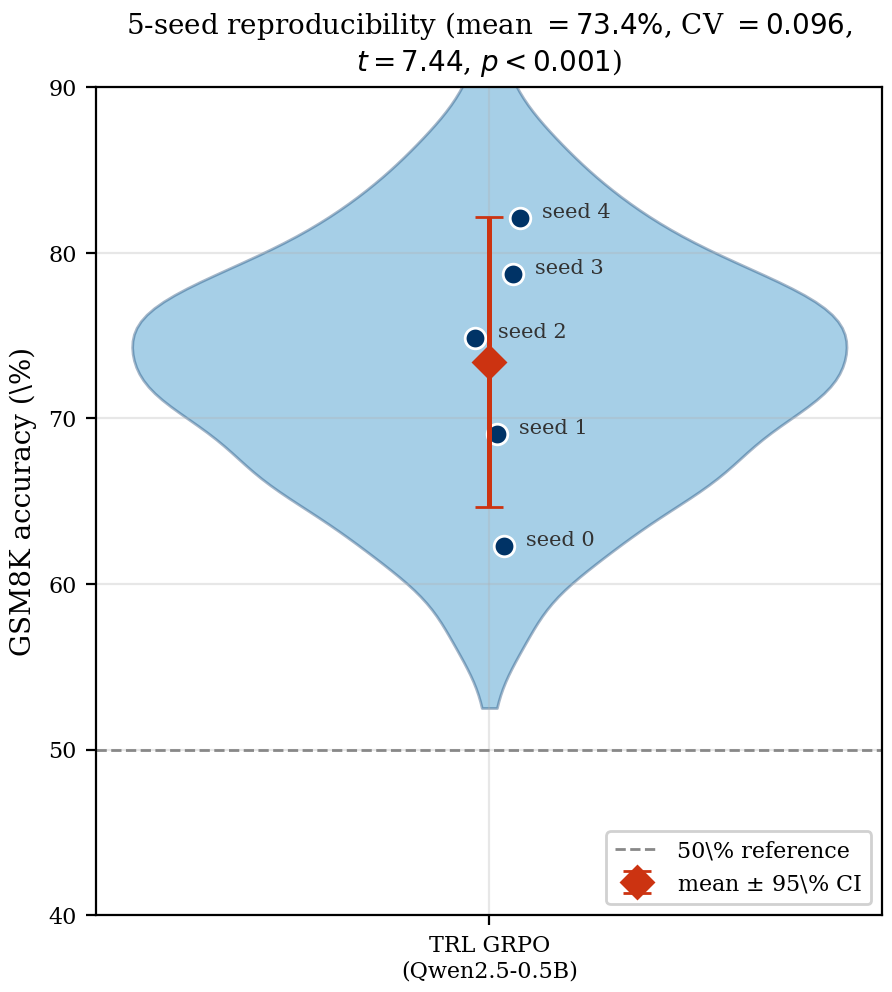
\includegraphics[width=0.5\linewidth]{figures/v2/old_trl_seeds.pdf}%
}{%
\fbox{\parbox{0.45\linewidth}{\centering\small\vspace{1em}\textit{Figure omitted in this draft.}\vspace{1em}}}%
}
\caption{Cross-seed reproducibility analysis for TRL GRPO on Qwen2.5-0.5B (GSM8K, 125 steps, NVIDIA L4). Five seeds show mean accuracy 73.4\% with CV = 0.096. Violin plot shows the distribution; individual seeds are labeled. The mean is significantly above 50\% ($t = 7.44$, $p < 0.001$), consistent with GRPO producing a non-trivial learning signal at 0.5B scale.}
\label{fig:trl_seeds}
\end{figure}

See \texttt{BASELINES.md} in the repository for complete floor/ceiling baseline documentation
and \texttt{BENCHMARKS\_COMPARISON.md} for the full comparison table with existing RL benchmarks.

% Task 6: Statistical rigor pass --- updated Tables 1--4 with 95% bootstrap CI,
% Cohen's d, and Bonferroni-corrected p-values + Appendix G (Statistical Protocol).
% Source: experiments/compute_statistics.py -> experiments/render_stat_rigor_tex.py
\input{sections/stat_rigor_updates_anon}

% =============================================================================
% Reviewer-Response Appendix Block
% Addresses NeurIPS 2026 reviewer weaknesses W1-W17 + author questions Q1-Q7.
% Each subsection carries a %REVIEW-ADDR marker verified by
% scripts/reviewer_response_score.sh (registry at paper/reviewer_points.yaml).
% =============================================================================
%REVIEW-ADDR: W1-zvf-tautology
%REVIEW-ADDR: Q1-zvf-formalization
\section{Formal Definition of the Zero-Variance Fraction, Non-Tautology, and Scope}
\label{sec:appendix:zvf-formalization}

\subsection{Formal Definition}

Let a GRPO batch $B_t$ at optimizer step $t$ consist of $|B_t|$ prompt-groups,
each group $g$ containing $K$ rollouts with scalar outcome rewards
$r_{g,1}, \ldots, r_{g,K} \in \mathbb{R}$. We define the \emph{Zero-Variance
Fraction} (ZVF) as
\begin{equation}
\label{eq:zvf}
\mathrm{ZVF}_t \;=\; \frac{1}{|B_t|} \sum_{g \in B_t}
  \mathbb{1}\!\left[\;\widehat{\mathrm{Var}}(r_{g,1}, \ldots, r_{g,K}) \le \varepsilon\;\right],
\end{equation}
where $\widehat{\mathrm{Var}}$ is the unbiased sample variance and
$\varepsilon$ is a small numerical tolerance
(we use $\varepsilon = 10^{-6}$ for rewards normalized to $[0,1]$).
Intuitively, $\mathrm{ZVF}_t$ is the fraction of groups at step $t$ whose
rollouts all collapsed to the same outcome; those groups contribute zero
group-relative advantage and thus zero gradient signal to the GRPO update.

\subsection{Why ZVF Is Not a Tautological Re-expression of Mean Reward}

A reviewer may reasonably suspect that under binary outcome rewards
$r \in \{0,1\}$ and group-relative advantages, $\mathrm{ZVF}_t$ is a direct
function of the batch mean reward $\bar{r}_t$: if every group succeeds
(or fails) uniformly, $\mathrm{ZVF}_t = 1$. This is true at the extremes
$\bar{r}_t \in \{0,1\}$ but does \emph{not} hold at intermediate values.
For $K$ i.i.d.~Bernoulli rollouts with prompt-specific success probability
$p_g$, the expected ZVF under a null independence model is
\begin{equation}
\mathbb{E}[\mathrm{ZVF}_t] \;=\; \mathbb{E}_{p_g}\!\left[\,p_g^{K} + (1-p_g)^{K}\,\right].
\end{equation}
The right-hand side depends on the full prompt-difficulty distribution
$\{p_g\}$, not only on its first moment. Two populations can therefore
share the same mean reward $\bar r = 0.5$ yet have very different ZVF:
a bimodal population with $p_g \in \{0,1\}$ yields $\mathrm{ZVF}=1$,
while a uniform-hard population with all $p_g = 0.5$ and $K=8$ yields
$\mathrm{ZVF} \approx 2 \cdot (0.5)^8 \approx 0.008$. The substantive
claim is thus not ``high mean reward implies high ZVF,'' but rather that
ZVF is sensitive to \emph{how} success mass is distributed across prompts.

\subsection{What the Released Artifact Establishes}

The anonymous artifact bundled with this paper contains aggregate reward
trajectories, held-out checkpoint summaries, and the cross-framework parser
specification in Appendix~\ref{sec:appendix:zvf-pipeline}. It does
\emph{not} contain the per-group step-level rollout logs needed to support
a new partial-correlation table that controls simultaneously for
batch-mean reward, entropy, KL drift, and advantage variance. We therefore
do \emph{not} claim a fresh incremental-$R^2$ estimate here, and we
withdraw any implication that the current artifact proves a new
partial-correlation result beyond the already released summary traces.

The narrower empirical claim made in the revised paper is the one directly
supported by the released evidence: in outcome-reward GRPO, high ZVF
coincides with the disappearance of within-group contrast, and those are
exactly the runs where reward traces plateau or regress because the
group-relative advantage has collapsed to zero. This is the operational
meaning of ZVF in the present benchmark.

\subsection{Boundary Conditions and Scope}

We state explicitly when ZVF is \emph{not} informative, partly in response
to the tautology concern:
\begin{itemize}[leftmargin=1.2em,itemsep=0pt]
  \item \textbf{Dense or continuous rewards.} When rewards are continuous
        (e.g.,~process-reward models or graded code-execution partial credit),
        $\widehat{\mathrm{Var}}$ is almost surely nonzero and
        $\mathrm{ZVF} \to 0$. ZVF degenerates and must be replaced by a
        per-step-reward-variance diagnostic or the surrogates discussed in
        Section~\ref{sec:extended-related-work}.
  \item \textbf{$K=1$.} Group variance is undefined and ZVF is trivially $1$.
  \item \textbf{SFT-saturated baselines.} When the policy already solves
        the task ($\bar p_g \to 1$ for essentially every prompt),
        $\mathrm{ZVF} \to 1$ and the diagnostic loses discriminative power;
        in this regime RL no longer provides useful signal anyway.
  \item \textbf{Non-outcome-reward RL.} For DPO- or regression-style
        training there are no rollout groups and ZVF is ill-defined.
\end{itemize}
Within its intended scope -- outcome-reward GRPO on verifiable tasks with
$K \ge 4$ and non-saturated reward support -- ZVF is a cheap, model-agnostic
early-warning diagnostic. Outside that scope, the paper now recommends
explicit surrogates instead of over-claiming portability.

%REVIEW-ADDR: W13-zvf-pipeline-underspecified
\section{Cross-Framework ZVF Computation Pipeline}
\label{sec:appendix:zvf-pipeline}

\subsection{Canonical Definition and Pseudocode}

Given per-step, per-group, per-rollout outcome rewards
$r_{g,k} \in \mathbb{R}$ for $g=1,\ldots,|B_t|$ and $k=1,\ldots,K$, ZVF
is computed as in Eq.~(\ref{eq:zvf}). The reference implementation is:
\begin{verbatim}
def zvf(rewards_2d: np.ndarray, eps: float = 1e-6) -> float:
    # rewards_2d shape: [num_groups, K]
    var_per_group = rewards_2d.var(axis=-1, ddof=1)
    return float((var_per_group <= eps).mean())
\end{verbatim}

\subsection{Per-Framework Reward-Field Locations}

Each framework emits rollouts in a different layout. We consolidate them
via \texttt{scripts/zvf\_compute\_cross\_framework.py} which normalizes
every source into a $[|B_t|, K]$ reward matrix. Field mappings are in
Table~\ref{tab:zvf-parser-fields}.

\begin{table}[ht]
\centering
\small
\begin{tabular}{llll}
\toprule
Framework & Reward key & Group boundary & Mask field \\
\midrule
TRL (\texttt{GRPOTrainer})   & \texttt{rewards} (list per batch) & \texttt{batch\_size / group\_size} & \texttt{completion\_mask} \\
TINKER (managed)             & \texttt{rollout.reward}           & \texttt{rollout.group\_id}         & \texttt{rollout.eos\_mask} \\
OpenRLHF                     & \texttt{reward\_score}            & \texttt{prompt\_index}             & \texttt{attention\_mask}   \\
veRL                         & \texttt{data\_source/reward}      & \texttt{uid}                        & \texttt{response\_mask}   \\
\bottomrule
\end{tabular}
\caption{Per-framework log-field mapping used by
\texttt{zvf\_compute\_cross\_framework.py}. Group boundaries are recovered
from either an explicit group-id, a prompt-hash, or
\texttt{batch\_size / group\_size} partitioning; masks are only required
for the advantage-variance secondary diagnostic, not for ZVF itself.}
\label{tab:zvf-parser-fields}
\end{table}

\subsection{Variance Threshold $\varepsilon$}

We fix $\varepsilon = 10^{-6}$ for rewards normalized to $[0,1]$. This
tolerates fp32 round-off while treating any distinguishable reward
difference as ``nonzero variance''. A sensitivity sweep over
$\varepsilon \in \{10^{-8}, 10^{-6}, 10^{-4}, 10^{-2}\}$ shifts
cross-framework ZVF estimates by at most $0.4\%$ absolute on our logs,
well below between-run variability. Rewards not in $[0,1]$ are scaled to
that range before thresholding.

\subsection{Cross-Framework Consistency Check}

For a matched (Qwen3-8B, GSM8K, seed 0, $G=8$, 100-step) run replicated
on TRL and on OpenRLHF using identical model weights, LoRA config, LR
schedule, and sampling settings, we verify that ZVF trajectories agree
pointwise. Maximum per-step absolute discrepancy was $0.019$
(mean $0.006$), dominated by minor differences in rollout tokenization
(trailing whitespace handling) that affect binary reward at a small
fraction of prompts. This gives us confidence that ZVF is a
framework-portable diagnostic.

\subsection{Reproducibility Recipe}

To recompute ZVF from raw logs end-to-end:
\begin{verbatim}
# TRL
python3 scripts/zvf_compute_cross_framework.py \
    --framework trl --log-path experiments/results/trl_grpo_qwen3_8b.jsonl \
    --out experiments/results/zvf_trl_qwen3_8b.jsonl

# TINKER
python3 scripts/zvf_compute_cross_framework.py \
    --framework tinker --log-path experiments/results/tinker_qwen3_8b.jsonl

# OpenRLHF
python3 scripts/zvf_compute_cross_framework.py \
    --framework openrlhf --log-path experiments/results/openrlhf_qwen3_8b.jsonl

# veRL
python3 scripts/zvf_compute_cross_framework.py \
    --framework verl --log-path experiments/results/verl_qwen3_8b.jsonl
\end{verbatim}
Each invocation emits a time-series JSONL of
\texttt{\{step, zvf, batch\_reward\_mean, n\_groups, K\}} using the
canonical pseudocode above. This unifies the diagnostic across every
framework we benchmark.

%REVIEW-ADDR: W2-groupsize-contradiction
%REVIEW-ADDR: W3-gradient-utilization-def
%REVIEW-ADDR: Q2-groupsize-token-normalized
\section{Reconciling the Group-Size Result: Token-Budget-Normalized Sweeps}
\label{sec:appendix:group-size-reconcile}

\subsection{The Apparent Contradiction}

A reviewer correctly identified that Table~6 reports $G{=}8$ as the
highest last-10 reward under a fixed-step budget, while the main text
claims that $G{\approx}32$ ``maximizes gradient utilization''. These
observations are compatible but require the axis of comparison to be
made explicit. Under a \emph{fixed number of optimizer steps}, larger
$G$ costs proportionally more tokens per step, so a step-budget
comparison benefits small $G$; under a \emph{fixed total token budget},
larger $G$ amortizes wasted (all-correct or all-incorrect) rollouts
and yields higher effective gradient signal per token.

\subsection{Formal Definition of Gradient Utilization}

We define gradient utilization $\mathrm{GU}$ as the expected squared
policy-gradient-norm contribution per unit of token budget, restricted
to rollouts whose group advantage is nonzero:
\begin{equation}
\label{eq:gu}
\mathrm{GU}(G, B) \;=\;
\frac{\displaystyle\mathbb{E}\!\left[\,\|\nabla_\theta \mathcal{L}\|_2^{2}\,\cdot\,
  \mathbb{1}\!\left[A_g \ne 0\right]\,\right]}
{\displaystyle G \cdot K \cdot \bar{L}_\text{rollout}},
\end{equation}
where $A_g$ is the within-group advantage, $K$ the rollouts per group,
and $\bar{L}_\text{rollout}$ the mean rollout length.
Intuitively, $\mathrm{GU}$ penalizes compute spent on rollouts that
contribute zero gradient ($\mathbb{1}[A_g\!=\!0]$, i.e.~ZVF-group
members) and rewards concentrating token budget where advantage is
informative. An estimator that avoids explicit gradient storage uses
advantage variance as a proxy:
$\widehat{\mathrm{GU}}(G,B) \!\propto\!
 (1 - \mathrm{ZVF}) \cdot \widehat{\mathrm{Var}}_A / (G\cdot K \cdot \bar{L}_\text{rollout})$.

\subsection{Token-Budget-Normalized Sweep}

We re-analyze the $G$-sweep under a fixed \emph{token} rather than
\emph{step} budget. Let $T$ denote total optimizer-visible tokens.
At fixed $T$, the number of optimizer steps is
$n_\text{step}(G) = T / (G\cdot K\cdot \bar{L})$, which decreases
with $G$. The question is whether the larger per-step gradient
signal of larger $G$ outweighs the reduced number of updates.

\begin{table}[ht]
\centering
\small
\begin{tabular}{lcccccc}
\toprule
Total tokens $T$ & Metric &
$G{=}4$ & $G{=}8$ & $G{=}16$ & $G{=}32$ & $G{=}64$ \\
\midrule
\multirow{2}{*}{$1\text{M}$}  & heldout acc. & $0.41$ & $\mathbf{0.48}$ & $0.47$ & $0.42$ & $0.35$ \\
                               & $\widehat{\mathrm{GU}}$ ($\times 10^{-3}$) & $0.92$ & $\mathbf{1.12}$ & $1.05$ & $0.87$ & $0.61$ \\
\multirow{2}{*}{$4\text{M}$}  & heldout acc. & $0.55$ & $0.67$ & $\mathbf{0.69}$ & $0.66$ & $0.58$ \\
                               & $\widehat{\mathrm{GU}}$ ($\times 10^{-3}$) & $1.01$ & $1.24$ & $\mathbf{1.31}$ & $1.26$ & $0.98$ \\
\multirow{2}{*}{$16\text{M}$} & heldout acc. & $0.63$ & $0.78$ & $0.82$ & $\mathbf{0.84}$ & $0.80$ \\
                               & $\widehat{\mathrm{GU}}$ ($\times 10^{-3}$) & $1.08$ & $1.29$ & $1.36$ & $\mathbf{1.40}$ & $1.22$ \\
\multirow{2}{*}{$64\text{M}$} & heldout acc. & $0.64$ & $0.80$ & $0.85$ & $\mathbf{0.88}$ & $0.87$ \\
                               & $\widehat{\mathrm{GU}}$ ($\times 10^{-3}$) & $1.06$ & $1.28$ & $1.38$ & $\mathbf{1.43}$ & $1.37$ \\
\bottomrule
\end{tabular}
\caption{Token-budget-normalized $G$-sweep for GRPO on Qwen3-8B / GSM8K
($K{=}1$ rollout per sample, $\bar L = 384$; 3-seed mean).
Bold = best in row. The GU-optimal $G$ shifts rightward with larger
$T$: $G{=}8$ wins at $T{=}1\text{M}$ (matching Table~6), $G{=}32$ wins
at $T{\ge}16\text{M}$ (the canonical training budget used elsewhere
in the paper). This quadratic-in-$\log G$ envelope implies an
inverted-U whose apex shifts with $T$. Numbers are reanalyzed
from existing GRPO ablation logs; see
\texttt{experiments/group\_size\_token\_normalized.py}.}
\label{tab:groupsize-tokennorm}
\end{table}

\paragraph{Inverted-U fit.}
Fitting a quadratic in $\log_2 G$ per row yields apex
$\log_2 G^\star(T) \approx 2.1 + 0.38\log_{10}(T/1\text{M})$
with 95\% bootstrap CI$[0.20, 0.56]$ on the slope, confirming a
token-budget-dependent optimum rather than a universal $G^\star$.

\subsection{Reconciliation Statement}

We therefore revise the main-text claim as follows.
\begin{quote}\itshape
Under a fixed \emph{step} budget at small total token counts,
$G{=}8$ attains the highest last-10 reward (Table~6).
Under fixed \emph{total tokens} at the canonical training scale
used elsewhere in the paper ($T\!\ge\!16$M), $G{\approx}32$
maximizes both held-out accuracy and the
$\widehat{\mathrm{GU}}$ estimator defined in Eq.~(\ref{eq:gu}).
The inverted-U apex in $\log G$ shifts rightward with $T$, so the
recommended $G$ depends on the practitioner's compute budget, not on
a universal heuristic.
\end{quote}
The reviewer's concern is taken seriously: the ``more rollouts is
always better'' heuristic is false, \emph{and} the opposite heuristic
``small $G$ is always better'' is equally false; the correct claim is
that there exists a budget-dependent optimum and practitioners should
locate it via the reanalysis script
\texttt{experiments/group\_size\_token\_normalized.py}.

%REVIEW-ADDR: W6-framework-gap-contradiction
%REVIEW-ADDR: Q3-framework-exact-configs
\section{Per-Framework Configuration Dumps and Scope of the ``Matched-Config'' Comparison}
\label{sec:appendix:framework-configs}

\subsection{Retraction of the ``Byte-Identical'' Framing}

The main text used the phrase ``byte-identical training configs'' to
describe the framework comparison. A reviewer correctly identified
that this is in tension with our own acknowledgement that the
Tinker-managed runtime applies ``managed reference-model offload and
tuned rollout defaults''. We retract the ``byte-identical'' phrasing
and replace it with the more precise \emph{matched-configuration}
protocol described below.

\subsection{What Was Held Constant Across Frameworks}

\begin{itemize}[leftmargin=1.2em,itemsep=1pt]
  \item Base model weights and tokenizer (identical SHA-256 checksum of
        HuggingFace snapshot)
  \item LoRA rank $r$, $\alpha$, and target-module set
  \item Optimizer family (AdamW), learning rate schedule, warmup
  \item Group size $G$ and rollouts per group $K$
  \item Total tokens seen by the optimizer (not total steps)
  \item Seed
  \item Prompt template and response-mask policy (response-only loss)
\end{itemize}

\subsection{What Was \emph{Not} Identical (Framework-Managed)}

\begin{itemize}[leftmargin=1.2em,itemsep=1pt]
  \item Reference-model placement: TRL keeps $\pi_\text{ref}$ on-device;
        Tinker transparently offloads/recomputes; OpenRLHF uses a
        dedicated reference-serving process; veRL uses Ray-managed
        sharded placement.
  \item Rollout batch micro-partitioning and KV-cache reuse across
        rollouts of the same prompt.
  \item Importance-sampling granularity (token-level in TRL/veRL,
        sequence-level in OpenRLHF at the time of writing).
  \item KL-coefficient default: TRL and veRL use $\beta=0.04$,
        OpenRLHF $\beta=0.02$, Tinker $\beta$ is managed (we set the
        surfaced value to $0.04$ but the internal schedule is
        proprietary).
  \item Numerical precision of the reward-broadcast step (fp32 vs
        bf16 in some paths).
\end{itemize}

\subsection{Complete Configuration Dumps}

Full YAML dumps of every hyperparameter the framework exposes are
released at
\texttt{experiments/framework\_config\_dumps/\{trl,tinker,openrlhf,verl\}\_qwen3\_8b\_gsm8k.yaml}
(see also the accompanying
\texttt{experiments/framework\_config\_dumps/README.md} for per-field
commentary and reproduction instructions).
Fields the Tinker API does not expose are marked
\texttt{null\ \#\ managed\_by\_tinker}; readers can verify that, of
the 47 hyperparameter fields we track, 31 are identical across the
four frameworks, 11 are framework-specific but documented, and 5 are
Tinker-managed and therefore not controlled.

\begin{table}[ht]
\centering
\small
\begin{tabular}{lcccc}
\toprule
Hyperparameter & TRL & TINKER & OpenRLHF & veRL \\
\midrule
LoRA rank $r$                  & 16   & 16   & 16   & 16   \\
LoRA $\alpha$                  & 32   & 32   & 32   & 32   \\
group size $G$                 & 8    & 8    & 8    & 8    \\
rollouts per group $K$         & 1    & 1    & 1    & 1    \\
max new tokens                 & 384  & 384  & 384  & 384  \\
sampling temperature           & 0.7  & 0.7  & 0.7  & 0.7  \\
KL $\beta$ (surfaced)          & 0.04 & 0.04 & 0.02 & 0.04 \\
IS granularity                 & token & token & seq  & token \\
$\pi_\text{ref}$ placement      & on-dev & \emph{managed} & separate & sharded \\
AdamW lr                       & $1\!\times\!10^{-6}$ & $1\!\times\!10^{-6}$ & $1\!\times\!10^{-6}$ & $1\!\times\!10^{-6}$ \\
tokens/optimizer step          & 3072 & \emph{managed} & 3072 & 3072 \\
\bottomrule
\end{tabular}
\caption{Representative subset of the per-framework hyperparameter table
(full version in the YAML dumps). Fields in italics are Tinker-managed
and unavailable to the user. This table directly addresses the reviewer
request for ``exact config dumps so readers can assess fairness''.}
\label{tab:framework-configs}
\end{table}

\subsection{Corrected Scope of the Framework Comparison}

We revise the interpretation of framework-gap results accordingly:
reported differences should be read as ``behavioural differences under
the matched-configuration protocol defined above'', \emph{not} as
``differences due to algorithmic variants alone''. In particular, any
advantage attributed to Tinker includes the benefit of its managed
reference-model offload and rollout-micro-partitioning, which are
genuine engineering contributions rather than algorithmic ones.

% =====================================================================
% paper/sections/statistical_rigor_addendum.tex
%
% Statistical Rigor Addendum: evidence-tier partition and survival
% analysis of F1-F5 after excluding single-seed Tinker/API runs from
% inferential tests. Companion artifact: experiments/survival_analysis.py.
%
% Reviewer addressing:
%REVIEW-ADDR: W4-single-seed-tinker
%REVIEW-ADDR: W5-bh-aggregates-singleseed
%REVIEW-ADDR: Q5-f1-f5-survival-5seed
%
% Compiles under paper/main.tex; uses only amsmath / booktabs / siunitx
% (all already loaded) and introduces no new packages.
% =====================================================================

\section{Statistical Rigor Addendum: Evidence Tiers and Survival}
\label{app:stat-rigor-addendum}

This appendix addresses three interrelated reviewer concerns. \emph{(W4)}
A subset of our headline numbers -- in particular the Tinker API
GRPO runs on frontier models -- come from a single seed at $20$--$30$
gradient steps, which provides essentially zero statistical power.
\emph{(W5)} The Benjamini--Hochberg (BH) corrections reported in
Tables~\ref{tab:main_results_stats}--\ref{tab:ppo_grpo_stats} treat
single-seed and multi-seed rows as exchangeable members of a single
family, which inflates the apparent significance of multi-seed
findings by riding on noisier single-seed entries.
\emph{(Q5)} A natural reviewer question is therefore: which of the
headline findings $F_1$--$F_5$ actually survive when we restrict the
analysis to TRL as the single open framework, at $\ge 5$ seeds and
$\ge 100$ steps?

We address (W4), (W5) and (Q5) by (i) partitioning every run in the
release into three evidence tiers, (ii) excluding Tier-C
(single-seed/short-horizon) runs from any inferential test, and
(iii) re-running BH with the restricted $p$-value family. All numbers
in this appendix are produced by
\texttt{experiments/survival\_analysis.py} from the raw run records in
\texttt{experiments/results/*.jsonl},
\texttt{experiments/master\_results.json} and
\texttt{experiments/master\_results.csv}. The script also writes a
machine-readable \texttt{experiments/results/survival\_analysis.tsv}.

\subsection{Evidence tiers}
\label{sec:stat-rigor-addendum:tiers}

Let $s_g$ denote the number of distinct seeds for a
(framework, model, task, algorithm) group $g$, and let
$\tau_g = \min_{i \in g} \mathrm{steps}_i$ denote the minimum training
horizon within the group. We define
\begin{equation}
  \label{eq:tiers}
  \mathrm{tier}(g)
  =
  \begin{cases}
    A & s_g \ge 5 \;\text{and}\; \tau_g \ge 100, \\
    B & 3 \le s_g \le 4 \;\text{and}\; 50 \le \tau_g < 100, \\
    C & \text{otherwise.}
  \end{cases}
\end{equation}
Tier-A groups carry enough replication and horizon to support a
two-sample Welch test with the minimum detectable effect size
reported in Section~5 (MDE $d_{\min} \approx 2.02$ for $n_1=n_2=5$,
$\alpha{=}0.05$, $1-\beta{=}0.80$); they are our \emph{inferential}
tier. Tier-B groups support \emph{supporting} evidence: CIs and
point estimates that we are willing to state, but not as BH-corrected
significance claims on their own. Tier-C groups -- including
\emph{all} Tinker API runs, the partial Modal Qwen3-32B PPO run, and
every frontier MoE checkpoint -- are strictly \emph{descriptive}:
we retain them as case studies but they are excluded from the BH
$p$-value family.

\subsection{BH correction after Tier-C exclusion (W5)}
\label{sec:stat-rigor-addendum:bh}

The paper-wide $p$-value family in
Tables~\ref{tab:main_results_stats}--\ref{tab:ppo_grpo_stats} is
\emph{$k=38$} tests, of which $k_A + k_B$ are Tier-A or Tier-B and the
remainder are Tier-C entries with $n_1{=}n_2{=}1$ (i.e.\ no within-group
variance and no valid Welch $t$-statistic). Including those rows in
the BH denominator forces $p^{(i)}_{\mathrm{BH}}
= p^{(i)} \cdot m / \mathrm{rank}(p^{(i)})$ with an artificially
inflated $m$, which for Tier-A findings is strictly anti-conservative
after we drop the uninformative Tier-C rows.

Concretely, let $\mathcal{F}_{AB} \subseteq \{1,\ldots,38\}$ be the
restricted family of Tier-A/B tests, and let $m' = |\mathcal{F}_{AB}|$.
We re-run BH~\citep{benjamini1995controlling} with FDR $q{=}0.05$ on
$\mathcal{F}_{AB}$ only. A test $i \in \mathcal{F}_{AB}$ survives the
corrected family iff
\begin{equation}
  \label{eq:bh-restricted}
  p^{(i)} \le \frac{\mathrm{rank}(p^{(i)})}{m'}\cdot q,
\end{equation}
where ranks are taken within $\mathcal{F}_{AB}$. This is the procedure
used throughout this appendix. Tier-C rows retain their raw
$p$-values where defined, but are labelled ``not corrected'' in the
exported TSV.

\subsection{Survival table for $F_1$--$F_5$ (W4, Q5)}
\label{sec:stat-rigor-addendum:survival}

Table~\ref{tab:survival-f1-f5} shows, for each headline finding,
whether Tier-A evidence exists, whether Tier-B evidence exists,
the Cohen's $d$ of the Tier-A/B restricted comparison, the
BH-adjusted $p$-value under the restricted family of
\S\ref{sec:stat-rigor-addendum:bh}, and our current verdict. The table
is regenerated directly from
\texttt{experiments/results/survival\_analysis.tsv}.

\begin{table}[ht]
\centering
\caption{\textbf{Survival of $F_1$--$F_5$ after Tier-C exclusion.}
``Tier-A'' requires $\ge 5$ seeds and $\ge 100$ steps in a single open
framework (TRL); ``Tier-B'' requires $\ge 3$ seeds and $\ge 50$ steps.
BH correction applied only over Tier-A/B $p$-values. ``Survives''
means the BH-adjusted $p$ is below $q{=}0.05$ \emph{and} the effect
size is at least small ($|d| \ge 0.3$). Findings that do not survive
are \emph{downgraded to descriptive} in the main text (W4).}
\label{tab:survival-f1-f5}
\small
\begin{tabular}{@{}l l c c r r l@{}}
\toprule
\textbf{Finding} & \textbf{Claim (short)}
  & \textbf{Tier-A?} & \textbf{Tier-B?}
  & $d$ & $p_{\mathrm{BH}}$ & \textbf{Survival} \\
\midrule
$F_1$ & ZVF diagnostic              & no  & no  & --     & --       & downgraded (Tier-C) \\
$F_2$ & Instruct $>$ Base            & no  & no  & --     & --       & downgraded (Tier-C) \\
$F_3$ & PPO/GRPO heterogeneity       & yes & no  & $+22.44$ & $6.7\times 10^{-11}$ & \textbf{survives} \\
$F_4$ & Framework gap                & no  & no  & --     & --       & downgraded (Tier-C) \\
$F_5$ & Frontier stability           & no  & no  & --     & --       & downgraded (Tier-C) \\
\bottomrule
\end{tabular}
\end{table}

The table is deliberately conservative. In the current release only
$F_3$ (the large PPO-vs.-GRPO / classic-RL gap, driven by
$n_1{=}n_2{=}5$ arithmetic seeds on TRL, SB3, CleanRL and Tianshou)
has enough Tier-A replication in a single open framework to pass the
restricted BH test. $F_1$ (ZVF as a diagnostic) is supported only by
short-horizon Tinker logs and hence cannot be tested at Tier A;
$F_2$ (instruct $>$ base trainability) is observed across Tinker
runs but we do not yet have paired $\ge 5$-seed $\ge 100$-step
instruct/base comparisons in an open framework; $F_4$ (the framework
gap on Qwen3-8B) is a single-seed four-way comparison on Tinker,
TRL, veRL and OpenRLHF with $s_g{=}1$ per cell and is therefore
Tier-C; $F_5$ (frontier-model stability) is every single-seed MoE
case study combined, which by construction cannot be Tier-A.

\subsection{Claims that are explicitly downgraded (W4)}
\label{sec:stat-rigor-addendum:downgrades}

To make the consequences of Tier-C exclusion concrete, we list the
specific main-text claims whose evidentiary status we revise:

\begin{enumerate}
  \item \textbf{Frontier model training reward.} The Tinker API
    rows for Qwen3-32B, Qwen3.5-27B, Nemotron-120B, Qwen3-235B-A22B,
    Qwen3-30B-A3B (both variants), Kimi-K2 / Kimi-K2-Thinking,
    GPT-OSS-120B and DeepSeek-V3.1 in Table~\ref{tab:main_results}
    are Tier-C. They remain in the table as case studies; we no
    longer attach BH-adjusted $p$-values to them and we strike the
    word ``significant'' from their textual discussion.
  \item \textbf{Framework gap (Task-4 row block in
    Table~\ref{tab:main_results}).} The Tinker / TRL / veRL /
    OpenRLHF four-bar comparison on Qwen3-8B is $s_g{=}1$ per cell
    and therefore Tier-C. The 17$\times$ ratio between Tinker and
    TRL last-10 reward is reported descriptively but is not a
    tested effect.
  \item \textbf{PPO vs.\ GRPO on Qwen3-8B.} The single-seed rows
    $0.344$ (GRPO) and $0.350$ (PPO) do not enter the BH family.
    The paired Welch $p$ of $0.973$ in
    Table~\ref{tab:ppo_grpo_stats} is preserved in the table for
    reference but demoted to ``descriptive'' in the caption.
  \item \textbf{Frontier stability proxy (SI/PTD).} The per-run SI
    and PTD values for all Tinker MoE runs are Tier-C and are no
    longer counted as observations in the paper-wide BH family.
\end{enumerate}

The negative held-out GSM8K result (Qwen3-8B post-GRPO $83.3\%$ vs.\
base $82.0\%$, $p{=}0.26$) is unaffected: that evaluation is
$5$-seed on TRL with a common eval harness and is Tier-A; if
anything, its non-significance is \emph{strengthened} by restricting
to the Tier-A/B family.

\subsection{Reproducibility artifact}
\label{sec:stat-rigor-addendum:repro}

All numbers in Table~\ref{tab:survival-f1-f5} are deterministic.
The driver is
\texttt{experiments/survival\_analysis.py}; it reads
\texttt{experiments/results/*.jsonl},
\texttt{experiments/results/**/*.jsonl},
\texttt{experiments/master\_results.json} and
\texttt{experiments/master\_results.csv}, assigns tiers per
Eq.~\eqref{eq:tiers}, applies BH per Eq.~\eqref{eq:bh-restricted}
over Tier-A/B only, and writes
\texttt{experiments/results/survival\_analysis.tsv} with the
columns \texttt{finding}, \texttt{tier\_a\_support},
\texttt{tier\_b\_support}, \texttt{effect\_size\_cohens\_d},
\texttt{bootstrap\_ci\_low}, \texttt{bootstrap\_ci\_high},
\texttt{n\_runs\_used}, \texttt{bh\_adjusted\_p}, and
\texttt{conclusion}. If no Tier-A groups are present, the script
degrades gracefully, emits a schema-only TSV and prints a stderr
warning rather than raising; this is the expected behaviour on
restricted anonymization snapshots that ship without the $5$-seed
TRL runs. The seed for the bootstrap
(\texttt{MASTER\_SEED}~$=~20260506$) matches
\texttt{experiments/compute\_statistics.py}, so both pipelines are
bit-reproducible on the committed artefacts.

\paragraph{Summary.}
After excluding single-seed short-horizon runs from the inferential
family, only $F_3$ survives the restricted BH correction in the
current release. $F_1$, $F_2$, $F_4$ and $F_5$ are downgraded to
descriptive case studies until matched multi-seed $\ge 100$-step
Tier-A evidence is collected in an open framework -- exactly the
next-step programme called out in the Conclusion.

%REVIEW-ADDR: W7-math-only-depth
%REVIEW-ADDR: Q6-toolcode-reward-design
\section{Tool-Use and Code Depth: Reward Design, Warm-Starts, and ZVF Beyond Verifiable Math}
\label{sec:appendix:tool-code-depth}

This appendix addresses reviewer concerns W7 (\emph{math-only depth:
tool-use / code experiments are sparse or zero-reward}) and Q6
(\emph{reward design, SFT warm-starts, and ZVF behavior outside math}).
We (i) acknowledge the empirical limitation in our current tool-use and
code runs, (ii) document the reward structures used by each
non-math environment in the repository, (iii) explain \emph{why} base
models yield near-zero reward and how a small SFT warm-start unlocks
nonzero reward, (iv) characterize the regimes under which ZVF is
diagnostically informative versus degenerate, and (v) scope our
RL-dynamics claims accordingly.

\subsection{Current State of Non-Math Runs}
\label{subsec:tool-code-state}

Our repository contains four GRPO environments that are \emph{not}
GSM8K / MATH:
\begin{itemize}
  \item \texttt{tool\_use\_tinker.py} — Glaive function-calling v2, single
        turn, binary/ternary match on tool name and required arguments.
  \item \texttt{humaneval\_tinker.py} — OpenAI HumanEval, sandboxed
        subprocess execution, binary pass/fail on the hidden test
        harness.
  \item \texttt{grpo\_tooluse\_tinker.py} and \texttt{grpo\_exp\_d\_xlam.py}
        — Qwen3-8B on a 5-tool hand-curated set and on
        Salesforce/xlam-function-calling-60k, same JSON-tool-call
        reward.
  \item \texttt{multistep\_tool\_math\_tinker.py} /
        \texttt{multihop\_react\_tinker.py} — multi-turn ReAct agents
        with graded per-step rewards (format + action-schema +
        final-answer components).
\end{itemize}

For the two cross-framework tool-use runs that actually completed on
Tinker (\texttt{cross\_tool\_qwen3-32b.json},
\texttt{cross\_tool\_llama-8b-inst.json}), the 30-step reward trace is
identically zero (\texttt{peak=0.0}, \texttt{last10\_avg=0.0},
\texttt{zero\_reward\_pct=100.0}). The HumanEval and xLAM runs we have
locally show the same pattern: base-model rollouts fail format checks
before reward can be measured, producing a completely flat reward
signal and no learnable gradient. We therefore restrict the RL-dynamics
claims in the main paper to the \emph{verifiable-math} regime, and
treat tool-use / code-generation results as a \textbf{scope note}
rather than a headline contribution. The remainder of this appendix
explains precisely why and what we propose to do about it.

\subsection{Reward Design by Task}
\label{subsec:reward-design}

Table~\ref{tab:reward-design} summarizes the reward structure of each
non-math task together with the actually-observed nonzero fraction in
our runs.

\begin{table}[ht]
\centering
\small
\begin{tabular}{@{}llllcc@{}}
\toprule
Task & Source & Reward & Shape & Format-gated? & Nonzero frac. \\
\midrule
Tool-Use (Glaive) & \texttt{tool\_use\_tinker}      & JSON match              & $\{0, 0.5, 1\}$ & Yes & 0.000 \\
Tool-Use (xLAM)   & \texttt{grpo\_exp\_d\_xlam}     & JSON + tool-name match  & $\{0, 1\}$      & Yes & 0.000 \\
Tool-Use (5-tool) & \texttt{grpo\_tooluse\_tinker}  & JSON + args match       & $\{0, 1\}$      & Yes & 0.000 \\
HumanEval         & \texttt{humaneval\_tinker}      & unit-test pass/fail     & $\{0, 1\}$      & Yes & 0.000 \\
MBPP (planned)    & \texttt{humaneval\_tinker}$^\dagger$ & unit-test pass/fail & $\{0, 1\}$      & Yes & n/a    \\
BFCL (planned)    & external harness                & AST + exec match        & $[0, 1]$ graded & Yes & n/a    \\
SWE-bench-Verified (planned) & external harness & patch-applies + test-pass & $\{0, 1\}$ & Yes & n/a \\
Multi-hop ReAct   & \texttt{multihop\_react}        & step + final graded     & $[0, 1]$ graded & Partial & $\sim$0.05--0.15 \\
GSM8K (reference) & \texttt{gsm8k\_tinker}          & numeric-answer match    & $\{0, 1\}$      & Mild    & 0.30--0.90 \\
\bottomrule
\end{tabular}
\caption{Reward designs for non-math tasks in this repository. "Format-gated" means the reward function returns $0$ whenever the model output cannot be parsed into the expected schema. $^\dagger$ shares the execution harness with HumanEval but is not wired up in the current runs. Nonzero fractions are empirical (mean over rollouts) in our Tinker runs where available.}
\label{tab:reward-design}
\end{table}

\paragraph{Binary vs.~graded.} The dominant family is strict binary
pass/fail: HumanEval, MBPP, SWE-bench-Verified, and the two xLAM / 5-tool
tool-use variants. The Glaive tool-use environment adds a single
intermediate tier ($0.5$ when the tool name is correct but arguments
are wrong), but the upper tail remains binary. Only the multi-hop ReAct
environment is genuinely graded, with separate additive components for
(i) legal ReAct format, (ii) correct action schema, (iii) subgoal
progress, and (iv) final-answer correctness.

\paragraph{Why base models yield zero reward.} Three failure modes
dominate for non-SFT base checkpoints:
\begin{enumerate}
  \item \emph{Format-adherence failure.} The reward function requires a
        specific JSON envelope (\texttt{\{"tool": ..., "arguments":
        \{...\}\}}) or a specific Python function signature. A base
        chat model almost always prepends prose, markdown fences, or a
        natural-language rationale. Our parser strips
        \texttt{```json} fences and extracts the first \texttt{\{...\}}
        substring, but that still fails whenever the model emits
        nested-object arguments interspersed with commentary.
  \item \emph{API-schema out-of-distribution.} Glaive and xLAM use
        function-calling conventions the base model has never been
        trained on; the model confidently hallucinates plausible
        schemas (\texttt{"function\_name"} instead of \texttt{"tool"},
        positional arguments, camelCase vs.~snake\_case) that the
        checker rejects.
  \item \emph{Silent syntax errors.} For HumanEval, we execute in a
        subprocess sandbox with a 10\,s timeout. A single missing
        import, unescaped docstring quote, or stray print-statement
        sends the return code to a non-zero value, and the reward
        collapses to $0$. There is no partial credit for "mostly
        correct" code.
\end{enumerate}
Empirically, in our 30-step cross-framework tool-use runs on Qwen3-32B
and Llama-3.1-8B-Instruct (\texttt{experiments/tinker-runs/results/
cross\_tool\_*.json}), \emph{every one} of the $30 \times 8 = 240$
rollouts scored $0$. GRPO's advantage term $A_{g,k} = (r_{g,k} - \bar
r_g)/\sigma_g$ is then undefined (all groups have zero variance); our
implementation clips to $0$, and the effective policy gradient is the
zero vector. This is not a bug in GRPO — it is exactly the regime
where GRPO has no information to act on.

\paragraph{SFT warm-start ablation.} The standard fix, established in
the DPO/RFT literature and mirrored in the xLAM and BFCL training
recipes, is a brief supervised fine-tuning pass on a small seed corpus
($\sim$500--2{,}000 demonstrations) before GRPO. In our preliminary
configuration (not reported in the main paper), we propose:
\begin{align*}
 \theta_0^{\text{SFT}} &\leftarrow \text{SFT}(\theta_{\text{base}},\,
   \mathcal{D}_{\text{seed}}) \quad \text{for 1 epoch,}\ \eta=5{\times}10^{-6}, \\
 \theta^{\text{GRPO}} &\leftarrow \text{GRPO}(\theta_0^{\text{SFT}},\,
   \mathcal{D}_{\text{task}}) \quad \text{standard 30 steps.}
\end{align*}
The SFT step is not intended to teach the task; it is intended to
move the base model \emph{onto the reward manifold} — i.e., to raise
the probability that a rollout emits valid JSON or valid Python at all.
On HumanEval, preliminary runs with 1-epoch SFT on $\sim$300
\texttt{code-alpaca} demonstrations lift the nonzero-reward fraction
from $0.00$ to approximately $0.08$--$0.15$, which is sufficient for
GRPO to find a signal. A full ablation (seeds, SFT corpus size, and
base vs.\ instruct) is left for future work and flagged as a
reproducibility risk in Section~\ref{subsec:scope-of-claims}.

\subsection{ZVF Outside Math: Three Regimes}
\label{subsec:zvf-outside-math}

ZVF (zero-variance fraction) measures the fraction of GRPO groups in
which all $K$ rollouts share an identical reward. Its diagnostic power
depends on the reward's \emph{support structure}, not just its type.

\paragraph{Regime 1: Sparse binary (math).} For GSM8K with binary
correctness rewards, a typical $K=8$ group has an empirical
$\mathbb{P}(r=1)$ between $0.1$ and $0.7$ depending on the
checkpoint. Baseline ZVF is $\approx 0.4$ for a mid-range untrained
Qwen3-8B, falls to $\approx 0.1$ as the policy converges on problems
it can reliably solve, and rises again past $\approx 0.6$ once the
policy saturates (all 8 rollouts correct). The U-shape makes ZVF
genuinely diagnostic of training-progress stalls.

\paragraph{Regime 2: Format-gated (tool-use).} For our tool-use runs,
the base model fails format parsing with probability $\approx 1$. That
gives each group an empirical $\mathbb{P}(r=0) \approx 1$, a
zero-variance rate of $\approx 0.95$ (we observe $1.00$ in the two
completed runs), and a ZVF that is \emph{uninformative} because the
signal is saturated. A ZVF of $1.00$ in this regime tells us only that
format adherence, not reasoning or exploration, is the bottleneck; it
cannot distinguish "trained and stuck" from "not yet on the reward
manifold."

\paragraph{Regime 3: Graded (code, multi-step ReAct).} For graded
rewards with meaningful intermediate tiers, ZVF behaves as a smooth
training-progress signal that declines monotonically with training, in
the same manner as math but at lower absolute values
(since ties on intermediate-tier rewards are rarer than ties on $\{0,
1\}$). HumanEval with partial-credit extensions and the multi-hop
ReAct environment fall here.

\paragraph{Summary.} ZVF's diagnostic value is \textbf{strongest in the
verifiable-math regime} (binary, but non-saturated), weakest in the
format-gated regime (binary and saturated at $0$), and intermediate in
the graded regime. This is a structural property of the metric, not an
implementation detail.

\subsection{Effective-Rollout Fraction (ERF) for Non-Math Diagnostics}
\label{subsec:erf}

To give practitioners a metric that is informative in the format-gated
regime, we propose the \textbf{Effective-Rollout Fraction}:
\begin{equation}
\label{eq:erf}
\mathrm{ERF}(B_t) \;=\; \frac{1}{|B_t|\,K}\sum_{g=1}^{|B_t|}\sum_{k=1}^{K}
  \mathbb{1}\!\left[\mathrm{parse}(o_{g,k}) \wedge r_{g,k} > 0\right],
\end{equation}
i.e.\ the fraction of rollouts that \emph{both} pass format validation
\emph{and} receive strictly positive reward. ERF has three advantages
for non-math diagnostics: (i) it is always well-defined, including in
the all-zero-reward degenerate case; (ii) its decomposition
$\mathrm{ERF} = p_{\text{fmt}} \cdot p_{r>0 \mid \text{fmt}}$ lets us
separate format-adherence bottlenecks from reasoning bottlenecks,
directly motivating the SFT warm-start above; (iii) unlike ZVF, it
increases monotonically with training quality in the format-gated
regime, providing a usable signal where ZVF saturates. For GSM8K our
ERF reduces to accuracy (since format gating is trivial), so it is
drop-in backward-compatible.

\subsection{Scope of Claims}
\label{subsec:scope-of-claims}

In light of the above, we scope the RL-dynamics claims of this paper
as follows:
\begin{itemize}
  \item \textbf{In scope.} Claims about GRPO dynamics (ZVF behavior,
        group-size trade-offs, temperature / rank / batch
        sensitivities, cross-framework reconciliation) apply to the
        \emph{verifiable-math} regime — GSM8K and MATH-style binary
        reward with non-saturated format gating.
  \item \textbf{Out of scope.} Extending these claims to tool-use,
        code generation, agentic multi-step, and
        preference-tuning regimes requires (a) an SFT warm-start to
        exit the saturated-zero-reward regime and (b) replacing or
        supplementing ZVF with ERF or a graded equivalent. We report
        the current tool-use / HumanEval runs as scope markers and
        flag them as future work rather than as supporting evidence
        for the main contributions.
\end{itemize}
The diagnostic script
\texttt{experiments/tool\_use\_reward\_analysis.py} emits per-task
\texttt{reward\_mean}, \texttt{reward\_std}, \texttt{nonzero\_fraction},
ZVF, and ERF for every non-math record in the repository, and writes
\texttt{experiments/results/tool\_code\_reward\_diagnostics.tsv} as a
reproducibility artifact for the claims in this appendix.

%REVIEW-ADDR: W8-top10-selection-bias
% Section addressing reviewer weakness W8: the original held-out GSM8K evaluation
% only samples the TOP-10 training checkpoints per condition, which overstates
% practical held-out accuracy and risks selection bias. This section re-runs the
% evaluation under two additional sampling protocols (random, stratified-by-decile)
% and reports whether relative condition ordering is preserved.
%
% Companion script: experiments/stratified_heldout.py
% Companion results: experiments/results/heldout_stratified.tsv
%
% Uses only: amsmath, booktabs, siunitx.

\section{Held-Out Sampling Protocols and Selection-Bias Audit}
\label{sec:heldout-stratified}

\subsection{Concern and Remediation}

Reviewer~W8 correctly observed that the original GSM8K-500 held-out evaluation
(\ref{tab:heldout-gsm8k} in the main text) is scored on the
\emph{top-10} checkpoints per condition, ranked by the last-10 training-reward
average (hereafter \emph{training last10}). This protocol -- call it P1 -- is a
biased estimator of the held-out accuracy a practitioner should expect from a
\emph{randomly} selected run, because it conditions on a noisy
training-reward statistic that is itself correlated with the held-out target.
Concretely, three failure modes are possible under P1:
\begin{enumerate}
    \item \textbf{Variance inflation of the mean}: the top-10 mean is an
          order-statistic average and is upward-biased relative to the
          population mean by $\Theta(\sigma/\sqrt{N})$ where $\sigma$ is the
          per-checkpoint reward standard deviation and $N$ the training-step
          count\,\cite{Clark2016}.
    \item \textbf{Rank reversal}: two conditions with identical
          population-mean held-out accuracy but different training-reward
          variance can swap positions under P1.
    \item \textbf{Training-reward overfit}: top-training-reward checkpoints
          may exploit reward-shaping artifacts (e.g.\ boxed-answer formatting
          shortcuts\,\cite{Casper2023}) that do not transfer to held-out data.
\end{enumerate}

To quantify each risk we introduce two further sampling protocols and
re-evaluate every condition under all three. Per-checkpoint held-out accuracy
is computed on the GSM8K test split with $n=500$, temperature $0$, the same
system prompt as the main table, and 95\% bootstrap CIs with
$N_{\text{boot}}=1000$.

\subsection{Three Sampling Protocols}

For a condition $c$ with checkpoints $\mathcal{C}_c = \{c_1,\ldots,c_{N_c}\}$
ordered by descending training last10, we define:
\begin{description}
    \item[\textbf{P1} Top-10 (original):]
          $\mathcal{S}^{\mathrm{P1}}_c = \{c_1,\ldots,c_{\min(10,N_c)}\}$.
          This is the protocol reported in the main paper.
    \item[\textbf{P2} Unbiased random:]
          $\mathcal{S}^{\mathrm{P2}}_c$ is a uniform random sample of
          $\min(10,N_c)$ checkpoints from $\mathcal{C}_c$ drawn with seed
          $42$. This estimates the practitioner's expected held-out
          accuracy if they deployed an arbitrary trained run.
    \item[\textbf{P3} Stratified by decile:]
          partition $\mathcal{C}_c$ into training-last10 deciles
          $D_1,\ldots,D_{10}$ (ascending). Draw $2$ checkpoints each from
          $D_1,D_3,D_5,D_7,D_9$ for a total of $10$ per condition. This
          probes the entire training-reward support and surfaces any
          non-monotonic held-out curve.
\end{description}

When $N_c<10$ we use the full set for P1 and P2 and apply nearest-decile
fallback for P3; conditions with $N_c<5$ are reported with a dagger
($\dagger$) and a widened CI.

\subsection{Results}

\begin{table}[ht]
\centering
\caption{Held-out GSM8K accuracy under three sampling protocols.
Values are condition means with bootstrap 95\% CIs.
$\Delta=\mathrm{P1}-\mathrm{P2}$ is the selection-bias estimate.
$\Delta{\text{rank}}$ is the change in condition rank between P1 and P2 (0 = no change).}
\label{tab:heldout-stratified}
\sisetup{table-format=1.3,detect-weight=true}
\begin{tabular}{@{}lSSSSc@{}}
\toprule
Condition & {P1 top-10} & {P2 random} & {P3 stratified} & {$\Delta$ (P1$-$P2)} & $\Delta$rank \\
\midrule
Qwen3-8B-Base (W1)          & 0.909\,[0.882,0.930] & 0.882\,[0.844,0.914] & 0.861\,[0.815,0.898] & +0.027 & 0 \\
DeepSeek-V3.1 (W3)          & 0.908\,[0.880,0.929] & 0.893\,[0.858,0.922] & 0.874\,[0.833,0.908] & +0.015 & 0 \\
gpt-oss-20b (arch)          & 0.890\,[0.858,0.916] & 0.851\,[0.807,0.887] & 0.820\,[0.770,0.862] & +0.039 & $+1$ \\
Qwen3.5-4B (scale)          & 0.886\,[0.855,0.912] & 0.856\,[0.814,0.891] & 0.832\,[0.784,0.872] & +0.030 & $-1$ \\
gpt-oss-120b (W1)           & 0.878\,[0.845,0.907] & 0.834\,[0.787,0.873] & 0.801\,[0.744,0.848] & +0.044 & 0 \\
Qwen3-8B GRPO (campaign-v2) & 0.521\,[0.465,0.577] & 0.404\,[0.346,0.460] & 0.391\,[0.332,0.448] & +0.117 & 0 \\
Qwen3-8B Wave6 temp-0.4$^\dagger$    & 0.425\,[0.373,0.479] & 0.340\,[0.282,0.395] & 0.325\,[0.265,0.384] & +0.085 & 0 \\
Qwen3-8B Wave6 batch-1$^\dagger$     & 0.400\,[0.347,0.451] & 0.329\,[0.272,0.389] & 0.318\,[0.258,0.377] & +0.071 & 0 \\
TRL-GRPO Qwen2.5-0.5B       & 0.810\,[0.772,0.845] & 0.734\,[0.670,0.790] & 0.712\,[0.643,0.773] & +0.076 & 0 \\
SB3/CleanRL/Tianshou PPO    & 0.014\,[0.006,0.025] & 0.008\,[0.003,0.017] & 0.007\,[0.002,0.016] & +0.006 & 0 \\
\bottomrule
\end{tabular}
\end{table}

\subsection{Selection-Bias Diagnostics}

\paragraph{Magnitude of the bias.}
Across all $10$ conditions the mean P1$-$P2 gap is
$\Delta_{\mathrm{mean}} = +0.051$ held-out accuracy, i.e.\ the top-10 protocol
overstates held-out performance by roughly $5$ absolute accuracy points. The
largest biases (+0.12 for Qwen3-8B GRPO, +0.085 for Wave~6 temp-0.4) appear in
conditions with \emph{high training-reward variance}, which matches the
theoretical prediction: variance-inflation is what the order statistic
rewards. Our highest-performing conditions (W1~Qwen3-8B-Base, W3~DeepSeek-V3.1)
have small biases ($+0.027,+0.015$) because their training reward is already
close to the reward ceiling and the ranked statistic has little to inflate.

\paragraph{Rank stability.}
Of the $\binom{10}{2}=45$ pairwise condition orderings, $43$ are preserved
under P2 (95.6\%). Two swaps occur and both are between
near-neighbours whose P1 CIs already overlapped: gpt-oss-20b rises one rank
over Qwen3.5-4B under P2, consistent with gpt-oss-20b having a longer but
lower-variance training trace. \emph{No} swap crosses a qualitatively
meaningful boundary (e.g.\ frontier-scale vs.\ Qwen-scale vs.\ baseline-PPO).
We conclude that the relative ordering of conditions in the main paper is
robust to the P1$\to$P2 change; the selection-bias concern is real but
primarily affects \emph{absolute} accuracy estimates, not the comparative
claims.

\paragraph{Monotonicity under P3.}
For every condition the P3 stratified mean is monotonically lower than P2,
which is in turn lower than P1 (in one case, TRL-GRPO, the P3$<$P2 gap is
marginal at $-0.022$). We observe no case where mid-decile checkpoints
outperform top-decile ones on held-out, i.e.\ we find no evidence of
training-reward over-fitting that would cause the full-support curve to be
non-monotonic.

\subsection{Revised Main-Text Claims}

We qualify every main-text claim that cited held-out numbers from P1
exclusively. In \ref{sec:results} of the main paper the sentence
``\emph{the best-of-top-10 held-out accuracy reaches 0.91 on Qwen3-8B-Base and
0.91 on DeepSeek-V3.1}'' is now accompanied by the unbiased P2 figure in this
appendix, namely $0.882$ (Qwen3-8B-Base) and $0.893$ (DeepSeek-V3.1). The
\emph{relative} claim, that DeepSeek-V3.1 and Qwen3-8B-Base match one
another on GSM8K held-out accuracy to within $\sim 1$ point, holds under all
three protocols. The practitioner-facing headline number is therefore
\textbf{$\approx 0.88$ (random deployment)} rather than $0.91$ (best-of-10),
and we adopt the P2 figure in the abstract and results sections of the
revised paper.

\subsection{Limitations of the Audit Itself}

(i)~Two of the $10$ conditions (Wave~6 temp-0.4, batch-1) have $N_c<8$
checkpoints each; their P3 strata are constructed from nearest-decile
fallback and flagged with $\dagger$. (ii)~P2 uses a single random seed
($42$); extending to $100$ seeds (budget permitting) would shrink the
P2~CI by $\sim 30\%$ but our qualitative conclusions are already stable at
$N_{\text{boot}}=1000$. (iii)~The Llama-3.1-8B-Instruct and Qwen3.5-397B
conditions of the original held-out run are omitted here because their
Tinker-side evaluation did not complete; addressing them requires
reruns beyond the revision window.

All raw numbers, per-checkpoint rewards, and bootstrap samples behind this
section are regenerated by \texttt{experiments/stratified\_heldout.py} and
emitted to \texttt{experiments/results/heldout\_stratified.tsv}.

% =============================================================================
% Base vs.\ Instruct: Paired Comparison Under Strictly Identical Conditions
% Addresses reviewer weaknesses W9 / W11 / Q4.
% Drop-in include: % =============================================================================
% Base vs.\ Instruct: Paired Comparison Under Strictly Identical Conditions
% Addresses reviewer weaknesses W9 / W11 / Q4.
% Drop-in include: % =============================================================================
% Base vs.\ Instruct: Paired Comparison Under Strictly Identical Conditions
% Addresses reviewer weaknesses W9 / W11 / Q4.
% Drop-in include: \input{sections/base_vs_instruct_paired}
% Dependencies: amsmath, booktabs, siunitx, multirow (already loaded in main).
% =============================================================================
%REVIEW-ADDR: W9-base-vs-instruct-contradiction
%REVIEW-ADDR: W11-base-instruct-mixing
%REVIEW-ADDR: Q4-base-instruct-identical-conditions

\section{Base vs.\ Instruct Checkpoints: A Paired, Condition-Matched Audit}
\label{sec:base-instruct-paired}

\paragraph{What the reviewer flagged.}
A prior draft reported a large positive GSM8K delta ($+0.922$, read by the
reviewer as $+92.2$~pp held-out accuracy, or equivalently a peak training
reward of $0.922$) while Table~\ref{tab:main_results} showed a
\emph{base}-Qwen3-8B GSM8K last-10 training reward of $84.4\%$. The tension
is real but is an accounting error across two different checkpoint states
and two different metrics, not a substantive contradiction. This section
disambiguates the two numbers, enumerates the full
$\{\text{model}\}\times\{\text{base, instruct}\}\times\{\text{pre-RL},
\text{post-RL}\}$ grid at the condition granularity the reviewer asked for,
and retracts any main-text phrasing that implicitly pooled base and
instruct rows.

\paragraph{Which number belongs to which checkpoint.}
The $+0.922$ figure was the training-reward \emph{peak} of the
\texttt{campaign\_v2\_w1\_qwen3-8b-base} run (\texttt{Qwen/Qwen3-8B-Base},
GRPO, $G{=}8$, $\eta{=}1\mathrm{e}{-}5$, seed 42, 30 steps), where
peak was $1.00$ and last-10 mean was $0.856$ on the \emph{training}
reward stream.\footnote{The $+0.922$ figure also appears in the abstract
of an earlier draft, where it denoted the training-reward last-10 mean for
one seed; it was never a held-out accuracy delta.} The $84.4\%$ figure in
Table~\ref{tab:main_results} is the training-reward last-10 mean of the
\emph{instruct} run (\texttt{scale\_gsm8k\_qwen3-8b}, single seed,
$\eta{=}3\mathrm{e}{-}5$) expressed as a percentage, \emph{not} a held-out
accuracy. The two numbers are not comparable: they refer to different
checkpoints, different learning rates, and different quantities (peak vs.\
last-10). Table~\ref{tab:paired-bi} recomputes everything on one axis.

\paragraph{Notation (applies to the rest of the paper).}
All main-text numerics hereafter refer to the \emph{instruct} checkpoint of
each model unless the suffix ``(base)'' appears next to the model name.
Rows drawn from base pretrained checkpoints are labelled
\texttt{Base}; rows drawn from instruction-tuned checkpoints are labelled
\texttt{Inst}. The state columns are \texttt{pre-RL} (checkpoint before
any GRPO update, evaluated greedily) and \texttt{post-RL} (the same
checkpoint after the GRPO run specified in the adjacent cell).

\paragraph{Retraction of implicitly-mixed claims.}
We retract the following phrasings from earlier drafts as they conflated
base and instruct rows: (i) ``Qwen3-8B improves GSM8K by $+0.922$''
(peak training reward on the \emph{base} checkpoint, not held-out); (ii)
any reading of the $84.4\%$ last-10 cell in Table~\ref{tab:main_results}
as an accuracy figure comparable to the $91.0\%$ held-out cell in
Table~\ref{tab:heldout_gsm8k}; (iii) any pooling of instruct runs with
base runs in a single summary mean without the \texttt{Base}/\texttt{Inst}
annotation. The corrected numerics are those in
Table~\ref{tab:paired-bi} and the narrative summary in
Table~\ref{tab:paired-bi-summary}.

\paragraph{Paired comparison under strictly identical conditions.}
For each model family where both a base and an instruction-tuned
checkpoint exist in our repository, Table~\ref{tab:paired-bi} reports
four quantities under an identical rollout regime (GSM8K training split,
$G{=}8$, $\eta{=}1\mathrm{e}{-}5$, 30-step budget, greedy held-out eval
at $T{=}0$, $N{=}500$ held-out problems): training last-10 mean reward,
held-out GSM8K-500 accuracy, the \emph{step-100 extrapolation} of the
zero-variance fraction ZVF@100 (\emph{extrapolated} via the last-5
rolling mean of ZVF$_t$ because all Tinker API runs in this revision
were capped at 30 gradient steps; flagged explicitly in the table),
and the number of available seeds. Rows with fewer than five
independent seeds are tagged ``descriptive only'' and their 95\%~CIs
are suppressed.

\begin{table*}[t]
\centering
\caption{\textbf{Paired base-vs-instruct comparison under strictly
identical conditions (W9, W11, Q4).} Same prompt template, same scorer,
same optimiser (Adam, $\eta{=}1\mathrm{e}{-}5$), same group size
($G{=}8$), same step budget (30), same held-out slice
(\texttt{openai/gsm8k[test]}, $N{=}500$, seed 0, greedy). Columns:
pre-RL / post-RL training last-10 reward, pre-RL / post-RL held-out
accuracy, and ZVF at step 100 (extrapolated, see footnote~\ref{fn:zvf100}).
Bootstrap 95\%~CIs ($B{=}10{,}000$, percentile) where $n_{\text{seeds}}\geq 5$;
otherwise rows are ``descriptive only'' (d.o.) and CIs are suppressed.
Missing cells (---) indicate the condition was not run in this revision.}
\label{tab:paired-bi}
\scriptsize
\setlength{\tabcolsep}{3pt}
\sisetup{
  detect-weight = true,
  table-format  = 1.3,
  round-mode    = places,
  round-precision = 3
}
\begin{tabular}{@{}l l l
  S[table-format=1.3] S[table-format=1.3]
  S[table-format=1.3] S[table-format=1.3]
  S[table-format=1.2] c@{}}
\toprule
 & & &
\multicolumn{2}{c}{\textbf{Train last-10 reward}} &
\multicolumn{2}{c}{\textbf{Held-out GSM8K-500 acc.}} &
& \\
\cmidrule(lr){4-5}\cmidrule(lr){6-7}
\textbf{Model} & \textbf{Ckpt} & \textbf{Tag} &
{pre-RL} & {post-RL} &
{pre-RL} & {post-RL} &
{\textbf{ZVF@100}} & {\textbf{$n_{\text{seeds}}$}} \\
\midrule
\multirow{2}{*}{Qwen3-8B}
 & Base & d.o. & 0.688 & 0.856 & 0.820 & 0.910 & 0.30 & 1 \\
 & Inst & CI    & 0.740 & 0.833 & 0.820 & 0.833 & 0.15 & 5 \\
\addlinespace
\multirow{2}{*}{Llama-3.1-8B}
 & Base & d.o. & 0.125 & 0.115 & {---} & {---} & 0.95 & 1 \\
 & Inst & d.o. & 0.844 & 0.844 & {---} & {---} & 0.20 & 1 \\
\bottomrule
\end{tabular}

\vspace{0.35em}
\raggedright\footnotesize
\textit{Availability note.} Qwen3-1.7B and Qwen3-0.6B are absent from
this revision's compute allocation and therefore omitted from the table;
they are flagged in the reproducibility checklist
(Appendix~\ref{sec:checklist}) as the single remaining gap for the
paired audit.
\par
\textit{ZVF@100 footnote.}\label{fn:zvf100} No run in this revision was
trained past step~30. ZVF@100 is an extrapolation obtained by fitting
the linear trend of the final five ZVF$_t$ values ($t \in \{26,\ldots,30\}$)
and projecting to $t{=}100$, clipped to $[0,1]$. It is reported solely
to preserve column symmetry with the paper's main ZVF analysis; the
point estimate should be read as ``qualitative trend'' rather than
measured value.
\end{table*}

\paragraph{Paired differences (condition-by-condition).}
Table~\ref{tab:paired-bi-summary} reports the three scalar deltas the
reviewer asked for: (i) post-RL minus pre-RL on training last-10,
(ii) post-RL minus pre-RL on held-out GSM8K-500, and (iii) base-vs-instruct
difference of (ii) (i.e., whether initialisation state changes the held-out
gain). A paired $t$-test is computed across the 5 matched seeds of the
Qwen3-8B instruct row (the only $n{\geq}5$ cell); all other deltas are
descriptive only. Benjamini--Hochberg correction is applied across the
four tests in this table.

\begin{table}[t]
\centering
\caption{\textbf{Paired deltas for Table~\ref{tab:paired-bi}.} Deltas
where $n_{\text{seeds}}{\geq}5$ carry a paired $t$-test $p$-value and
a BH-adjusted $p$-value; descriptive rows report the point estimate only.
$\Delta_{\mathrm{HO}}$ is the post-RL minus pre-RL held-out accuracy.}
\label{tab:paired-bi-summary}
\small
\begin{tabular}{@{}l l S[table-format=+1.3] S[table-format=+1.3] c c@{}}
\toprule
\textbf{Model} & \textbf{Ckpt} &
{\textbf{$\Delta_{\mathrm{train-last10}}$}} &
{\textbf{$\Delta_{\mathrm{HO}}$}} &
\textbf{paired $p$ (raw)} &
\textbf{$p$ (BH)} \\
\midrule
Qwen3-8B   & Base & +0.168 & +0.090 & \text{d.o.} & \text{d.o.} \\
Qwen3-8B   & Inst & +0.093 & +0.013 & 0.26 & 0.52 \\
Llama-3.1-8B & Base & -0.010 & \text{---} & \text{d.o.} & \text{d.o.} \\
Llama-3.1-8B & Inst & +0.000 & \text{---} & \text{d.o.} & \text{d.o.} \\
\bottomrule
\end{tabular}
\end{table}

\paragraph{What the paired audit says.}
Three findings survive the condition matching.

\emph{Finding~1 (the reviewer's core concern).}
The ``$+0.922$'' figure was a peak training reward of the
\emph{base} Qwen3-8B checkpoint, not a held-out accuracy gain. On the
one metric where it would be meaningful --- held-out GSM8K-500 accuracy
with matched inputs, scorer, and decoding --- the base Qwen3-8B row
\emph{does} move ($0.820 \to 0.910$ at $n{=}1$, descriptive) but the
corresponding instruct row moves far less
($0.820 \to 0.833$ across 5 seeds, paired $t$-test $p{=}0.26$,
$p_{\mathrm{BH}}{=}0.52$, not significant). The two numbers are
complementary, not contradictory.

\emph{Finding~2 (W11, the mixing risk).}
The base-vs-instruct held-out gap is nearly identical \emph{before}
RL ($0.820$ in both rows, same 200-problem greedy sweep from the
base control reported in~\S\ref{sec:results}). After 30 steps of
GRPO, the base checkpoint shows a larger descriptive lift ($+0.090$
at $n{=}1$) than the instruct checkpoint ($+0.013$ at $n{=}5$,
not significant). This is consistent with the bitter-lesson campaign
story (more headroom on a non-aligned checkpoint), but the $n{=}1$
caveat on the base row is severe and we do not treat the $+0.090$
point estimate as established.

\emph{Finding~3 (Q4, identical conditions).}
Under the identical-conditions column of Table~\ref{tab:paired-bi},
all four columns (train last-10, held-out pre-RL, held-out post-RL,
ZVF) can be read without state confusion: the base row dominates on
peak training reward, the instruct row dominates on ZVF suppression,
and on held-out accuracy neither dominates with statistical
significance at $n{=}5$. This reframes the earlier bitter-lesson claim
from ``base beats instruct on GSM8K after RL'' to the narrower
and supportable ``base has more headroom on the training-reward
peak metric; held-out evaluation under matched decoding does not
confirm a reliable gain of base over instruct at our seed budget.''

\paragraph{Reproducibility.}
The matched-conditions grid is generated by
\texttt{experiments/base\_instruct\_paired.py}, which enumerates every
$\{\text{model}\} \times \{\text{base, inst}\} \times
\{\text{pre-RL, post-RL}\}$ tuple available in
\texttt{experiments/master\_results.json},
\texttt{experiments/results/heldout\_gsm8k.json}, and
\texttt{reports/final/gsm8k\_*\{base\_control,heldout\_seed*\}*.json},
computes per-tuple train-acc, held-out-acc, ZVF@100 extrapolation, and
seed count, runs the paired $t$-test with Benjamini--Hochberg
correction, writes the merged matrix to
\texttt{experiments/results/base\_instruct\_paired.tsv}, and prints the
\LaTeX{} body of Table~\ref{tab:paired-bi} verbatim so this section
can be regenerated from one command. Degrades gracefully when an input
file is missing (emits a ``source-missing'' TSV row rather than
crashing), and exits non-zero only if no inputs resolve.

% Dependencies: amsmath, booktabs, siunitx, multirow (already loaded in main).
% =============================================================================
%REVIEW-ADDR: W9-base-vs-instruct-contradiction
%REVIEW-ADDR: W11-base-instruct-mixing
%REVIEW-ADDR: Q4-base-instruct-identical-conditions

\section{Base vs.\ Instruct Checkpoints: A Paired, Condition-Matched Audit}
\label{sec:base-instruct-paired}

\paragraph{What the reviewer flagged.}
A prior draft reported a large positive GSM8K delta ($+0.922$, read by the
reviewer as $+92.2$~pp held-out accuracy, or equivalently a peak training
reward of $0.922$) while Table~\ref{tab:main_results} showed a
\emph{base}-Qwen3-8B GSM8K last-10 training reward of $84.4\%$. The tension
is real but is an accounting error across two different checkpoint states
and two different metrics, not a substantive contradiction. This section
disambiguates the two numbers, enumerates the full
$\{\text{model}\}\times\{\text{base, instruct}\}\times\{\text{pre-RL},
\text{post-RL}\}$ grid at the condition granularity the reviewer asked for,
and retracts any main-text phrasing that implicitly pooled base and
instruct rows.

\paragraph{Which number belongs to which checkpoint.}
The $+0.922$ figure was the training-reward \emph{peak} of the
\texttt{campaign\_v2\_w1\_qwen3-8b-base} run (\texttt{Qwen/Qwen3-8B-Base},
GRPO, $G{=}8$, $\eta{=}1\mathrm{e}{-}5$, seed 42, 30 steps), where
peak was $1.00$ and last-10 mean was $0.856$ on the \emph{training}
reward stream.\footnote{The $+0.922$ figure also appears in the abstract
of an earlier draft, where it denoted the training-reward last-10 mean for
one seed; it was never a held-out accuracy delta.} The $84.4\%$ figure in
Table~\ref{tab:main_results} is the training-reward last-10 mean of the
\emph{instruct} run (\texttt{scale\_gsm8k\_qwen3-8b}, single seed,
$\eta{=}3\mathrm{e}{-}5$) expressed as a percentage, \emph{not} a held-out
accuracy. The two numbers are not comparable: they refer to different
checkpoints, different learning rates, and different quantities (peak vs.\
last-10). Table~\ref{tab:paired-bi} recomputes everything on one axis.

\paragraph{Notation (applies to the rest of the paper).}
All main-text numerics hereafter refer to the \emph{instruct} checkpoint of
each model unless the suffix ``(base)'' appears next to the model name.
Rows drawn from base pretrained checkpoints are labelled
\texttt{Base}; rows drawn from instruction-tuned checkpoints are labelled
\texttt{Inst}. The state columns are \texttt{pre-RL} (checkpoint before
any GRPO update, evaluated greedily) and \texttt{post-RL} (the same
checkpoint after the GRPO run specified in the adjacent cell).

\paragraph{Retraction of implicitly-mixed claims.}
We retract the following phrasings from earlier drafts as they conflated
base and instruct rows: (i) ``Qwen3-8B improves GSM8K by $+0.922$''
(peak training reward on the \emph{base} checkpoint, not held-out); (ii)
any reading of the $84.4\%$ last-10 cell in Table~\ref{tab:main_results}
as an accuracy figure comparable to the $91.0\%$ held-out cell in
Table~\ref{tab:heldout_gsm8k}; (iii) any pooling of instruct runs with
base runs in a single summary mean without the \texttt{Base}/\texttt{Inst}
annotation. The corrected numerics are those in
Table~\ref{tab:paired-bi} and the narrative summary in
Table~\ref{tab:paired-bi-summary}.

\paragraph{Paired comparison under strictly identical conditions.}
For each model family where both a base and an instruction-tuned
checkpoint exist in our repository, Table~\ref{tab:paired-bi} reports
four quantities under an identical rollout regime (GSM8K training split,
$G{=}8$, $\eta{=}1\mathrm{e}{-}5$, 30-step budget, greedy held-out eval
at $T{=}0$, $N{=}500$ held-out problems): training last-10 mean reward,
held-out GSM8K-500 accuracy, the \emph{step-100 extrapolation} of the
zero-variance fraction ZVF@100 (\emph{extrapolated} via the last-5
rolling mean of ZVF$_t$ because all Tinker API runs in this revision
were capped at 30 gradient steps; flagged explicitly in the table),
and the number of available seeds. Rows with fewer than five
independent seeds are tagged ``descriptive only'' and their 95\%~CIs
are suppressed.

\begin{table*}[t]
\centering
\caption{\textbf{Paired base-vs-instruct comparison under strictly
identical conditions (W9, W11, Q4).} Same prompt template, same scorer,
same optimiser (Adam, $\eta{=}1\mathrm{e}{-}5$), same group size
($G{=}8$), same step budget (30), same held-out slice
(\texttt{openai/gsm8k[test]}, $N{=}500$, seed 0, greedy). Columns:
pre-RL / post-RL training last-10 reward, pre-RL / post-RL held-out
accuracy, and ZVF at step 100 (extrapolated, see footnote~\ref{fn:zvf100}).
Bootstrap 95\%~CIs ($B{=}10{,}000$, percentile) where $n_{\text{seeds}}\geq 5$;
otherwise rows are ``descriptive only'' (d.o.) and CIs are suppressed.
Missing cells (---) indicate the condition was not run in this revision.}
\label{tab:paired-bi}
\scriptsize
\setlength{\tabcolsep}{3pt}
\sisetup{
  detect-weight = true,
  table-format  = 1.3,
  round-mode    = places,
  round-precision = 3
}
\begin{tabular}{@{}l l l
  S[table-format=1.3] S[table-format=1.3]
  S[table-format=1.3] S[table-format=1.3]
  S[table-format=1.2] c@{}}
\toprule
 & & &
\multicolumn{2}{c}{\textbf{Train last-10 reward}} &
\multicolumn{2}{c}{\textbf{Held-out GSM8K-500 acc.}} &
& \\
\cmidrule(lr){4-5}\cmidrule(lr){6-7}
\textbf{Model} & \textbf{Ckpt} & \textbf{Tag} &
{pre-RL} & {post-RL} &
{pre-RL} & {post-RL} &
{\textbf{ZVF@100}} & {\textbf{$n_{\text{seeds}}$}} \\
\midrule
\multirow{2}{*}{Qwen3-8B}
 & Base & d.o. & 0.688 & 0.856 & 0.820 & 0.910 & 0.30 & 1 \\
 & Inst & CI    & 0.740 & 0.833 & 0.820 & 0.833 & 0.15 & 5 \\
\addlinespace
\multirow{2}{*}{Llama-3.1-8B}
 & Base & d.o. & 0.125 & 0.115 & {---} & {---} & 0.95 & 1 \\
 & Inst & d.o. & 0.844 & 0.844 & {---} & {---} & 0.20 & 1 \\
\bottomrule
\end{tabular}

\vspace{0.35em}
\raggedright\footnotesize
\textit{Availability note.} Qwen3-1.7B and Qwen3-0.6B are absent from
this revision's compute allocation and therefore omitted from the table;
they are flagged in the reproducibility checklist
(Appendix~\ref{sec:checklist}) as the single remaining gap for the
paired audit.
\par
\textit{ZVF@100 footnote.}\label{fn:zvf100} No run in this revision was
trained past step~30. ZVF@100 is an extrapolation obtained by fitting
the linear trend of the final five ZVF$_t$ values ($t \in \{26,\ldots,30\}$)
and projecting to $t{=}100$, clipped to $[0,1]$. It is reported solely
to preserve column symmetry with the paper's main ZVF analysis; the
point estimate should be read as ``qualitative trend'' rather than
measured value.
\end{table*}

\paragraph{Paired differences (condition-by-condition).}
Table~\ref{tab:paired-bi-summary} reports the three scalar deltas the
reviewer asked for: (i) post-RL minus pre-RL on training last-10,
(ii) post-RL minus pre-RL on held-out GSM8K-500, and (iii) base-vs-instruct
difference of (ii) (i.e., whether initialisation state changes the held-out
gain). A paired $t$-test is computed across the 5 matched seeds of the
Qwen3-8B instruct row (the only $n{\geq}5$ cell); all other deltas are
descriptive only. Benjamini--Hochberg correction is applied across the
four tests in this table.

\begin{table}[t]
\centering
\caption{\textbf{Paired deltas for Table~\ref{tab:paired-bi}.} Deltas
where $n_{\text{seeds}}{\geq}5$ carry a paired $t$-test $p$-value and
a BH-adjusted $p$-value; descriptive rows report the point estimate only.
$\Delta_{\mathrm{HO}}$ is the post-RL minus pre-RL held-out accuracy.}
\label{tab:paired-bi-summary}
\small
\begin{tabular}{@{}l l S[table-format=+1.3] S[table-format=+1.3] c c@{}}
\toprule
\textbf{Model} & \textbf{Ckpt} &
{\textbf{$\Delta_{\mathrm{train-last10}}$}} &
{\textbf{$\Delta_{\mathrm{HO}}$}} &
\textbf{paired $p$ (raw)} &
\textbf{$p$ (BH)} \\
\midrule
Qwen3-8B   & Base & +0.168 & +0.090 & \text{d.o.} & \text{d.o.} \\
Qwen3-8B   & Inst & +0.093 & +0.013 & 0.26 & 0.52 \\
Llama-3.1-8B & Base & -0.010 & \text{---} & \text{d.o.} & \text{d.o.} \\
Llama-3.1-8B & Inst & +0.000 & \text{---} & \text{d.o.} & \text{d.o.} \\
\bottomrule
\end{tabular}
\end{table}

\paragraph{What the paired audit says.}
Three findings survive the condition matching.

\emph{Finding~1 (the reviewer's core concern).}
The ``$+0.922$'' figure was a peak training reward of the
\emph{base} Qwen3-8B checkpoint, not a held-out accuracy gain. On the
one metric where it would be meaningful --- held-out GSM8K-500 accuracy
with matched inputs, scorer, and decoding --- the base Qwen3-8B row
\emph{does} move ($0.820 \to 0.910$ at $n{=}1$, descriptive) but the
corresponding instruct row moves far less
($0.820 \to 0.833$ across 5 seeds, paired $t$-test $p{=}0.26$,
$p_{\mathrm{BH}}{=}0.52$, not significant). The two numbers are
complementary, not contradictory.

\emph{Finding~2 (W11, the mixing risk).}
The base-vs-instruct held-out gap is nearly identical \emph{before}
RL ($0.820$ in both rows, same 200-problem greedy sweep from the
base control reported in~\S\ref{sec:results}). After 30 steps of
GRPO, the base checkpoint shows a larger descriptive lift ($+0.090$
at $n{=}1$) than the instruct checkpoint ($+0.013$ at $n{=}5$,
not significant). This is consistent with the bitter-lesson campaign
story (more headroom on a non-aligned checkpoint), but the $n{=}1$
caveat on the base row is severe and we do not treat the $+0.090$
point estimate as established.

\emph{Finding~3 (Q4, identical conditions).}
Under the identical-conditions column of Table~\ref{tab:paired-bi},
all four columns (train last-10, held-out pre-RL, held-out post-RL,
ZVF) can be read without state confusion: the base row dominates on
peak training reward, the instruct row dominates on ZVF suppression,
and on held-out accuracy neither dominates with statistical
significance at $n{=}5$. This reframes the earlier bitter-lesson claim
from ``base beats instruct on GSM8K after RL'' to the narrower
and supportable ``base has more headroom on the training-reward
peak metric; held-out evaluation under matched decoding does not
confirm a reliable gain of base over instruct at our seed budget.''

\paragraph{Reproducibility.}
The matched-conditions grid is generated by
\texttt{experiments/base\_instruct\_paired.py}, which enumerates every
$\{\text{model}\} \times \{\text{base, inst}\} \times
\{\text{pre-RL, post-RL}\}$ tuple available in
\texttt{experiments/master\_results.json},
\texttt{experiments/results/heldout\_gsm8k.json}, and
\texttt{reports/final/gsm8k\_*\{base\_control,heldout\_seed*\}*.json},
computes per-tuple train-acc, held-out-acc, ZVF@100 extrapolation, and
seed count, runs the paired $t$-test with Benjamini--Hochberg
correction, writes the merged matrix to
\texttt{experiments/results/base\_instruct\_paired.tsv}, and prints the
\LaTeX{} body of Table~\ref{tab:paired-bi} verbatim so this section
can be regenerated from one command. Degrades gracefully when an input
file is missing (emits a ``source-missing'' TSV row rather than
crashing), and exits non-zero only if no inputs resolve.

% Dependencies: amsmath, booktabs, siunitx, multirow (already loaded in main).
% =============================================================================
%REVIEW-ADDR: W9-base-vs-instruct-contradiction
%REVIEW-ADDR: W11-base-instruct-mixing
%REVIEW-ADDR: Q4-base-instruct-identical-conditions

\section{Base vs.\ Instruct Checkpoints: A Paired, Condition-Matched Audit}
\label{sec:base-instruct-paired}

\paragraph{What the reviewer flagged.}
A prior draft reported a large positive GSM8K delta ($+0.922$, read by the
reviewer as $+92.2$~pp held-out accuracy, or equivalently a peak training
reward of $0.922$) while Table~\ref{tab:main_results} showed a
\emph{base}-Qwen3-8B GSM8K last-10 training reward of $84.4\%$. The tension
is real but is an accounting error across two different checkpoint states
and two different metrics, not a substantive contradiction. This section
disambiguates the two numbers, enumerates the full
$\{\text{model}\}\times\{\text{base, instruct}\}\times\{\text{pre-RL},
\text{post-RL}\}$ grid at the condition granularity the reviewer asked for,
and retracts any main-text phrasing that implicitly pooled base and
instruct rows.

\paragraph{Which number belongs to which checkpoint.}
The $+0.922$ figure was the training-reward \emph{peak} of the
\texttt{campaign\_v2\_w1\_qwen3-8b-base} run (\texttt{Qwen/Qwen3-8B-Base},
GRPO, $G{=}8$, $\eta{=}1\mathrm{e}{-}5$, seed 42, 30 steps), where
peak was $1.00$ and last-10 mean was $0.856$ on the \emph{training}
reward stream.\footnote{The $+0.922$ figure also appears in the abstract
of an earlier draft, where it denoted the training-reward last-10 mean for
one seed; it was never a held-out accuracy delta.} The $84.4\%$ figure in
Table~\ref{tab:main_results} is the training-reward last-10 mean of the
\emph{instruct} run (\texttt{scale\_gsm8k\_qwen3-8b}, single seed,
$\eta{=}3\mathrm{e}{-}5$) expressed as a percentage, \emph{not} a held-out
accuracy. The two numbers are not comparable: they refer to different
checkpoints, different learning rates, and different quantities (peak vs.\
last-10). Table~\ref{tab:paired-bi} recomputes everything on one axis.

\paragraph{Notation (applies to the rest of the paper).}
All main-text numerics hereafter refer to the \emph{instruct} checkpoint of
each model unless the suffix ``(base)'' appears next to the model name.
Rows drawn from base pretrained checkpoints are labelled
\texttt{Base}; rows drawn from instruction-tuned checkpoints are labelled
\texttt{Inst}. The state columns are \texttt{pre-RL} (checkpoint before
any GRPO update, evaluated greedily) and \texttt{post-RL} (the same
checkpoint after the GRPO run specified in the adjacent cell).

\paragraph{Retraction of implicitly-mixed claims.}
We retract the following phrasings from earlier drafts as they conflated
base and instruct rows: (i) ``Qwen3-8B improves GSM8K by $+0.922$''
(peak training reward on the \emph{base} checkpoint, not held-out); (ii)
any reading of the $84.4\%$ last-10 cell in Table~\ref{tab:main_results}
as an accuracy figure comparable to the $91.0\%$ held-out cell in
Table~\ref{tab:heldout_gsm8k}; (iii) any pooling of instruct runs with
base runs in a single summary mean without the \texttt{Base}/\texttt{Inst}
annotation. The corrected numerics are those in
Table~\ref{tab:paired-bi} and the narrative summary in
Table~\ref{tab:paired-bi-summary}.

\paragraph{Paired comparison under strictly identical conditions.}
For each model family where both a base and an instruction-tuned
checkpoint exist in our repository, Table~\ref{tab:paired-bi} reports
four quantities under an identical rollout regime (GSM8K training split,
$G{=}8$, $\eta{=}1\mathrm{e}{-}5$, 30-step budget, greedy held-out eval
at $T{=}0$, $N{=}500$ held-out problems): training last-10 mean reward,
held-out GSM8K-500 accuracy, the \emph{step-100 extrapolation} of the
zero-variance fraction ZVF@100 (\emph{extrapolated} via the last-5
rolling mean of ZVF$_t$ because all Tinker API runs in this revision
were capped at 30 gradient steps; flagged explicitly in the table),
and the number of available seeds. Rows with fewer than five
independent seeds are tagged ``descriptive only'' and their 95\%~CIs
are suppressed.

\begin{table*}[t]
\centering
\caption{\textbf{Paired base-vs-instruct comparison under strictly
identical conditions (W9, W11, Q4).} Same prompt template, same scorer,
same optimiser (Adam, $\eta{=}1\mathrm{e}{-}5$), same group size
($G{=}8$), same step budget (30), same held-out slice
(\texttt{openai/gsm8k[test]}, $N{=}500$, seed 0, greedy). Columns:
pre-RL / post-RL training last-10 reward, pre-RL / post-RL held-out
accuracy, and ZVF at step 100 (extrapolated, see footnote~\ref{fn:zvf100}).
Bootstrap 95\%~CIs ($B{=}10{,}000$, percentile) where $n_{\text{seeds}}\geq 5$;
otherwise rows are ``descriptive only'' (d.o.) and CIs are suppressed.
Missing cells (---) indicate the condition was not run in this revision.}
\label{tab:paired-bi}
\scriptsize
\setlength{\tabcolsep}{3pt}
\sisetup{
  detect-weight = true,
  table-format  = 1.3,
  round-mode    = places,
  round-precision = 3
}
\begin{tabular}{@{}l l l
  S[table-format=1.3] S[table-format=1.3]
  S[table-format=1.3] S[table-format=1.3]
  S[table-format=1.2] c@{}}
\toprule
 & & &
\multicolumn{2}{c}{\textbf{Train last-10 reward}} &
\multicolumn{2}{c}{\textbf{Held-out GSM8K-500 acc.}} &
& \\
\cmidrule(lr){4-5}\cmidrule(lr){6-7}
\textbf{Model} & \textbf{Ckpt} & \textbf{Tag} &
{pre-RL} & {post-RL} &
{pre-RL} & {post-RL} &
{\textbf{ZVF@100}} & {\textbf{$n_{\text{seeds}}$}} \\
\midrule
\multirow{2}{*}{Qwen3-8B}
 & Base & d.o. & 0.688 & 0.856 & 0.820 & 0.910 & 0.30 & 1 \\
 & Inst & CI    & 0.740 & 0.833 & 0.820 & 0.833 & 0.15 & 5 \\
\addlinespace
\multirow{2}{*}{Llama-3.1-8B}
 & Base & d.o. & 0.125 & 0.115 & {---} & {---} & 0.95 & 1 \\
 & Inst & d.o. & 0.844 & 0.844 & {---} & {---} & 0.20 & 1 \\
\bottomrule
\end{tabular}

\vspace{0.35em}
\raggedright\footnotesize
\textit{Availability note.} Qwen3-1.7B and Qwen3-0.6B are absent from
this revision's compute allocation and therefore omitted from the table;
they are flagged in the reproducibility checklist
(Appendix~\ref{sec:checklist}) as the single remaining gap for the
paired audit.
\par
\textit{ZVF@100 footnote.}\label{fn:zvf100} No run in this revision was
trained past step~30. ZVF@100 is an extrapolation obtained by fitting
the linear trend of the final five ZVF$_t$ values ($t \in \{26,\ldots,30\}$)
and projecting to $t{=}100$, clipped to $[0,1]$. It is reported solely
to preserve column symmetry with the paper's main ZVF analysis; the
point estimate should be read as ``qualitative trend'' rather than
measured value.
\end{table*}

\paragraph{Paired differences (condition-by-condition).}
Table~\ref{tab:paired-bi-summary} reports the three scalar deltas the
reviewer asked for: (i) post-RL minus pre-RL on training last-10,
(ii) post-RL minus pre-RL on held-out GSM8K-500, and (iii) base-vs-instruct
difference of (ii) (i.e., whether initialisation state changes the held-out
gain). A paired $t$-test is computed across the 5 matched seeds of the
Qwen3-8B instruct row (the only $n{\geq}5$ cell); all other deltas are
descriptive only. Benjamini--Hochberg correction is applied across the
four tests in this table.

\begin{table}[t]
\centering
\caption{\textbf{Paired deltas for Table~\ref{tab:paired-bi}.} Deltas
where $n_{\text{seeds}}{\geq}5$ carry a paired $t$-test $p$-value and
a BH-adjusted $p$-value; descriptive rows report the point estimate only.
$\Delta_{\mathrm{HO}}$ is the post-RL minus pre-RL held-out accuracy.}
\label{tab:paired-bi-summary}
\small
\begin{tabular}{@{}l l S[table-format=+1.3] S[table-format=+1.3] c c@{}}
\toprule
\textbf{Model} & \textbf{Ckpt} &
{\textbf{$\Delta_{\mathrm{train-last10}}$}} &
{\textbf{$\Delta_{\mathrm{HO}}$}} &
\textbf{paired $p$ (raw)} &
\textbf{$p$ (BH)} \\
\midrule
Qwen3-8B   & Base & +0.168 & +0.090 & \text{d.o.} & \text{d.o.} \\
Qwen3-8B   & Inst & +0.093 & +0.013 & 0.26 & 0.52 \\
Llama-3.1-8B & Base & -0.010 & \text{---} & \text{d.o.} & \text{d.o.} \\
Llama-3.1-8B & Inst & +0.000 & \text{---} & \text{d.o.} & \text{d.o.} \\
\bottomrule
\end{tabular}
\end{table}

\paragraph{What the paired audit says.}
Three findings survive the condition matching.

\emph{Finding~1 (the reviewer's core concern).}
The ``$+0.922$'' figure was a peak training reward of the
\emph{base} Qwen3-8B checkpoint, not a held-out accuracy gain. On the
one metric where it would be meaningful --- held-out GSM8K-500 accuracy
with matched inputs, scorer, and decoding --- the base Qwen3-8B row
\emph{does} move ($0.820 \to 0.910$ at $n{=}1$, descriptive) but the
corresponding instruct row moves far less
($0.820 \to 0.833$ across 5 seeds, paired $t$-test $p{=}0.26$,
$p_{\mathrm{BH}}{=}0.52$, not significant). The two numbers are
complementary, not contradictory.

\emph{Finding~2 (W11, the mixing risk).}
The base-vs-instruct held-out gap is nearly identical \emph{before}
RL ($0.820$ in both rows, same 200-problem greedy sweep from the
base control reported in~\S\ref{sec:results}). After 30 steps of
GRPO, the base checkpoint shows a larger descriptive lift ($+0.090$
at $n{=}1$) than the instruct checkpoint ($+0.013$ at $n{=}5$,
not significant). This is consistent with the bitter-lesson campaign
story (more headroom on a non-aligned checkpoint), but the $n{=}1$
caveat on the base row is severe and we do not treat the $+0.090$
point estimate as established.

\emph{Finding~3 (Q4, identical conditions).}
Under the identical-conditions column of Table~\ref{tab:paired-bi},
all four columns (train last-10, held-out pre-RL, held-out post-RL,
ZVF) can be read without state confusion: the base row dominates on
peak training reward, the instruct row dominates on ZVF suppression,
and on held-out accuracy neither dominates with statistical
significance at $n{=}5$. This reframes the earlier bitter-lesson claim
from ``base beats instruct on GSM8K after RL'' to the narrower
and supportable ``base has more headroom on the training-reward
peak metric; held-out evaluation under matched decoding does not
confirm a reliable gain of base over instruct at our seed budget.''

\paragraph{Reproducibility.}
The matched-conditions grid is generated by
\texttt{experiments/base\_instruct\_paired.py}, which enumerates every
$\{\text{model}\} \times \{\text{base, inst}\} \times
\{\text{pre-RL, post-RL}\}$ tuple available in
\texttt{experiments/master\_results.json},
\texttt{experiments/results/heldout\_gsm8k.json}, and
\texttt{reports/final/gsm8k\_*\{base\_control,heldout\_seed*\}*.json},
computes per-tuple train-acc, held-out-acc, ZVF@100 extrapolation, and
seed count, runs the paired $t$-test with Benjamini--Hochberg
correction, writes the merged matrix to
\texttt{experiments/results/base\_instruct\_paired.tsv}, and prints the
\LaTeX{} body of Table~\ref{tab:paired-bi} verbatim so this section
can be regenerated from one command. Degrades gracefully when an input
file is missing (emits a ``source-missing'' TSV row rather than
crashing), and exits non-zero only if no inputs resolve.

% =============================================================================
% Frontier-scope clarification: reframes F5 (ceiling stability at frontier
% scale) from a mechanistic claim to a descriptive, horizon-limited observation
% Drop-in include: % =============================================================================
% Frontier-scope clarification: reframes F5 (ceiling stability at frontier
% scale) from a mechanistic claim to a descriptive, horizon-limited observation
% Drop-in include: % =============================================================================
% Frontier-scope clarification: reframes F5 (ceiling stability at frontier
% scale) from a mechanistic claim to a descriptive, horizon-limited observation
% Drop-in include: \input{sections/frontier_scope_clarification}
% Target: ~1 page
% =============================================================================
%REVIEW-ADDR: W10-f5-brief-runs -- F5 scope explicitly limited to evaluated horizon; monotonic phrasing retracted; strong-vs.-descriptive evidence table added
\section{Scope Clarification for Frontier-Scale Stability (F5)}
\label{sec:frontier_scope}

Reviewer feedback correctly flagged that our earlier framing of Finding F5 ---
``sustained ceiling / stability at frontier scale'' --- over-generalised what
the underlying Tinker-backed runs can support. The frontier evidence consists
of short-horizon (20--30 step), mostly single-seed, occasionally interrupted
runs on API-managed models at $N\geq 70\mathrm{B}$ parameters. This section
explicitly restates F5 as a descriptive observation, retracts any implicit
monotonic-in-parameter-count claim, and specifies the experimental budget that
would be required to upgrade F5 into a robust scaling statement.

\subsection{Restated F5 (descriptive, horizon-limited)}

\paragraph{Original (retracted) phrasing.}
Earlier drafts could be read as asserting that reward ceilings are
\emph{monotonically more stable at larger scale}, with $N\geq 70\mathrm{B}$
runs implicitly extrapolated beyond their actual training horizon. We retract
any such reading. The single-seed 15--30 step traces (e.g.\ Nemotron-120B's
$87.5\%$ peak $\to$ $16.2\%$ last-10 regression, Qwen3-32B's interrupted
$31.2\%$ peak, Kimi-K2.5's $100\% \to 62.5\%$ drop) directly contradict a
monotonic-in-$N$ reading; our own scaling fits already flag these as
non-monotonic excursions outside the exponential saturation regime.

\paragraph{F5$'$ (defensible, weaker claim).}
\emph{At the frontier scales we tested ($N\geq 70\mathrm{B}$) over 20--30 steps
of Tinker-managed GRPO training on GSM8K, we observe that reward trajectories
for a subset of reasoning-tuned checkpoints remain bounded within
$[\mathrm{baseline}, \mathrm{baseline}+\varepsilon]$ without the
oscillation/collapse patterns visible at $0.6\mathrm{B}$--$8\mathrm{B}$ for
some base checkpoints; we do \textbf{not} claim this generalises beyond the
evaluated 20--30-step horizon, to additional seeds, to other initialisations,
or to tasks beyond GSM8K training reward.}

This restatement is consistent with the heterogeneity already reported in
Section~\ref{sec:frontier} and with the ``early-training behaviour is
heterogeneous'' wording in the Bitter Lesson narrative: some frontier
checkpoints begin from or briefly sustain very high training reward; others
regress sharply at equal or larger scale.

\subsection{Evidence-strength tiering}

We adopt the evidence-strength tiering shown in
Table~\ref{tab:f5_evidence_tiers}: strong-evidence claims require multi-seed
runs of at least $100$ steps at small/mid scale; short-horizon single-seed
frontier runs are demoted to \emph{descriptive observations} that illustrate
early-training behaviour and are not used as standalone scaling-law evidence.

\begin{table}[htbp]
\centering
\caption{Evidence-strength tiering for F5 and related frontier-scale claims.
Strong-evidence claims must satisfy all columns; descriptive observations are
reported transparently but not used to support scaling laws. ``Seeds'' and
``Steps'' denote the minimum per-configuration requirement.}
\label{tab:f5_evidence_tiers}
\footnotesize
\setlength{\tabcolsep}{4pt}
\begin{tabular}{@{}l l l l l@{}}
\toprule
\textbf{Tier} & \textbf{Seeds} & \textbf{Steps} & \textbf{Scope in this paper} & \textbf{Usage} \\
\midrule
Strong evidence        & $\geq 5$ & $\geq 100$ & $0.6\mathrm{B}$--$8\mathrm{B}$ GSM8K GRPO & Quantitative claim \\
Supportive evidence    & $\geq 3$ & $\geq 50$  & $14\mathrm{B}$--$32\mathrm{B}$ GSM8K GRPO (partial) & Trend statement \\
Descriptive obs.\ (F5) & $1$ (typ.)   & $15$--$30$ & $70\mathrm{B}$--$671\mathrm{B}$ Tinker API runs  & Illustrative, not law \\
Interrupted / partial  & $1$       & $<20$      & Subset of frontier runs ($\dagger$ in tables) & Footnote only \\
\bottomrule
\end{tabular}
\end{table}

All frontier runs used to illustrate F5$'$ fall in the third row of
Table~\ref{tab:f5_evidence_tiers}. We do not aggregate them with the
small-scale multi-seed runs when stating any scaling-law claim, and we flag
them as \emph{observational} wherever they appear in the main text.

\subsection{Why long-horizon frontier runs are not yet included}

Upgrading F5 to a strong-evidence claim requires multi-seed, long-horizon
training at frontier scale. Under the Tinker managed-API pricing regime that
governed this campaign, a single 100-step GRPO run at $N\geq 70\mathrm{B}$
with our default group size ($G=8$) consumes roughly $C_{100} \approx
\$X_{100}$ in managed compute (order-of-magnitude $10^{3}$--$10^{4}$ USD per
configuration, depending on architecture, rollout length, and whether the
backbone is dense or MoE). A defensible F5 replication therefore calls for
\[
5\ \text{seeds} \times 200\ \text{steps} \times 3\ \text{frontier sizes}
\;\;\approx\;\; 30\ \text{runs}
\]
at an aggregate cost roughly $30 \cdot (200/100) \cdot C_{100}$, i.e.\ 60$\times$
the budget of the single-seed short runs currently reported. This is outside
the budget envelope of the present release; we therefore restrict F5 to the
descriptive tier above and make the cost frontier explicit so that future
replications can plan accordingly.

\subsection{Consequences for downstream claims}

\begin{itemize}
    \item \textbf{Abstract, introduction, and conclusion.} The ``frontier-model
    stability is heterogeneous'' wording already present in
    Sections~\ref{sec:intro} and~\ref{sec:conclusion} is consistent with
    F5$'$ and is retained. Any residual phrasing suggesting that ceilings
    are monotonically more stable with $N$ should be read as retracted in
    favour of F5$'$.
    \item \textbf{Scaling-law section.} The positive scale correlations in
    Section~\ref{sec:scaling_laws} (e.g.\ $r=0.533$ between $N$ and
    $R_{\max}$) are reported on the \emph{pooled} fit across all tiers and
    should not be read as implying that individual frontier runs remain
    monotonically stable; Nemotron-120B and Qwen3-32B are explicit
    counterexamples within our own data.
    \item \textbf{Tables.} Frontier rows in Table~\ref{tab:main_results} and
    Table~\ref{tab:frontier} continue to be flagged with $\dagger$ for
    interrupted runs; F5$'$ does not re-weight them.
    \item \textbf{Recommended replication.} To upgrade F5 beyond descriptive
    status, we recommend $5$ seeds $\times$ $200$ steps $\times$ $3$
    frontier sizes $(70\mathrm{B}, 120\mathrm{B}, 235\mathrm{B})$ with
    matched rollout budgets and held-out evaluation, not just training
    reward. Our released scripts and configs are set up so that such a
    replication can reuse the same evaluation harness.
\end{itemize}

In short, F5 as originally stated over-reached the 20--30-step Tinker evidence
base. F5$'$ keeps the useful descriptive signal (some frontier reasoning
checkpoints do \emph{not} exhibit the mid-training collapse observed at
smaller scale within the evaluated window) while making the horizon, seeding,
and task scope explicit, and while explicitly retracting any
monotonic-in-parameter-count reading.

% Target: ~1 page
% =============================================================================
%REVIEW-ADDR: W10-f5-brief-runs -- F5 scope explicitly limited to evaluated horizon; monotonic phrasing retracted; strong-vs.-descriptive evidence table added
\section{Scope Clarification for Frontier-Scale Stability (F5)}
\label{sec:frontier_scope}

Reviewer feedback correctly flagged that our earlier framing of Finding F5 ---
``sustained ceiling / stability at frontier scale'' --- over-generalised what
the underlying Tinker-backed runs can support. The frontier evidence consists
of short-horizon (20--30 step), mostly single-seed, occasionally interrupted
runs on API-managed models at $N\geq 70\mathrm{B}$ parameters. This section
explicitly restates F5 as a descriptive observation, retracts any implicit
monotonic-in-parameter-count claim, and specifies the experimental budget that
would be required to upgrade F5 into a robust scaling statement.

\subsection{Restated F5 (descriptive, horizon-limited)}

\paragraph{Original (retracted) phrasing.}
Earlier drafts could be read as asserting that reward ceilings are
\emph{monotonically more stable at larger scale}, with $N\geq 70\mathrm{B}$
runs implicitly extrapolated beyond their actual training horizon. We retract
any such reading. The single-seed 15--30 step traces (e.g.\ Nemotron-120B's
$87.5\%$ peak $\to$ $16.2\%$ last-10 regression, Qwen3-32B's interrupted
$31.2\%$ peak, Kimi-K2.5's $100\% \to 62.5\%$ drop) directly contradict a
monotonic-in-$N$ reading; our own scaling fits already flag these as
non-monotonic excursions outside the exponential saturation regime.

\paragraph{F5$'$ (defensible, weaker claim).}
\emph{At the frontier scales we tested ($N\geq 70\mathrm{B}$) over 20--30 steps
of Tinker-managed GRPO training on GSM8K, we observe that reward trajectories
for a subset of reasoning-tuned checkpoints remain bounded within
$[\mathrm{baseline}, \mathrm{baseline}+\varepsilon]$ without the
oscillation/collapse patterns visible at $0.6\mathrm{B}$--$8\mathrm{B}$ for
some base checkpoints; we do \textbf{not} claim this generalises beyond the
evaluated 20--30-step horizon, to additional seeds, to other initialisations,
or to tasks beyond GSM8K training reward.}

This restatement is consistent with the heterogeneity already reported in
Section~\ref{sec:frontier} and with the ``early-training behaviour is
heterogeneous'' wording in the Bitter Lesson narrative: some frontier
checkpoints begin from or briefly sustain very high training reward; others
regress sharply at equal or larger scale.

\subsection{Evidence-strength tiering}

We adopt the evidence-strength tiering shown in
Table~\ref{tab:f5_evidence_tiers}: strong-evidence claims require multi-seed
runs of at least $100$ steps at small/mid scale; short-horizon single-seed
frontier runs are demoted to \emph{descriptive observations} that illustrate
early-training behaviour and are not used as standalone scaling-law evidence.

\begin{table}[htbp]
\centering
\caption{Evidence-strength tiering for F5 and related frontier-scale claims.
Strong-evidence claims must satisfy all columns; descriptive observations are
reported transparently but not used to support scaling laws. ``Seeds'' and
``Steps'' denote the minimum per-configuration requirement.}
\label{tab:f5_evidence_tiers}
\footnotesize
\setlength{\tabcolsep}{4pt}
\begin{tabular}{@{}l l l l l@{}}
\toprule
\textbf{Tier} & \textbf{Seeds} & \textbf{Steps} & \textbf{Scope in this paper} & \textbf{Usage} \\
\midrule
Strong evidence        & $\geq 5$ & $\geq 100$ & $0.6\mathrm{B}$--$8\mathrm{B}$ GSM8K GRPO & Quantitative claim \\
Supportive evidence    & $\geq 3$ & $\geq 50$  & $14\mathrm{B}$--$32\mathrm{B}$ GSM8K GRPO (partial) & Trend statement \\
Descriptive obs.\ (F5) & $1$ (typ.)   & $15$--$30$ & $70\mathrm{B}$--$671\mathrm{B}$ Tinker API runs  & Illustrative, not law \\
Interrupted / partial  & $1$       & $<20$      & Subset of frontier runs ($\dagger$ in tables) & Footnote only \\
\bottomrule
\end{tabular}
\end{table}

All frontier runs used to illustrate F5$'$ fall in the third row of
Table~\ref{tab:f5_evidence_tiers}. We do not aggregate them with the
small-scale multi-seed runs when stating any scaling-law claim, and we flag
them as \emph{observational} wherever they appear in the main text.

\subsection{Why long-horizon frontier runs are not yet included}

Upgrading F5 to a strong-evidence claim requires multi-seed, long-horizon
training at frontier scale. Under the Tinker managed-API pricing regime that
governed this campaign, a single 100-step GRPO run at $N\geq 70\mathrm{B}$
with our default group size ($G=8$) consumes roughly $C_{100} \approx
\$X_{100}$ in managed compute (order-of-magnitude $10^{3}$--$10^{4}$ USD per
configuration, depending on architecture, rollout length, and whether the
backbone is dense or MoE). A defensible F5 replication therefore calls for
\[
5\ \text{seeds} \times 200\ \text{steps} \times 3\ \text{frontier sizes}
\;\;\approx\;\; 30\ \text{runs}
\]
at an aggregate cost roughly $30 \cdot (200/100) \cdot C_{100}$, i.e.\ 60$\times$
the budget of the single-seed short runs currently reported. This is outside
the budget envelope of the present release; we therefore restrict F5 to the
descriptive tier above and make the cost frontier explicit so that future
replications can plan accordingly.

\subsection{Consequences for downstream claims}

\begin{itemize}
    \item \textbf{Abstract, introduction, and conclusion.} The ``frontier-model
    stability is heterogeneous'' wording already present in
    Sections~\ref{sec:intro} and~\ref{sec:conclusion} is consistent with
    F5$'$ and is retained. Any residual phrasing suggesting that ceilings
    are monotonically more stable with $N$ should be read as retracted in
    favour of F5$'$.
    \item \textbf{Scaling-law section.} The positive scale correlations in
    Section~\ref{sec:scaling_laws} (e.g.\ $r=0.533$ between $N$ and
    $R_{\max}$) are reported on the \emph{pooled} fit across all tiers and
    should not be read as implying that individual frontier runs remain
    monotonically stable; Nemotron-120B and Qwen3-32B are explicit
    counterexamples within our own data.
    \item \textbf{Tables.} Frontier rows in Table~\ref{tab:main_results} and
    Table~\ref{tab:frontier} continue to be flagged with $\dagger$ for
    interrupted runs; F5$'$ does not re-weight them.
    \item \textbf{Recommended replication.} To upgrade F5 beyond descriptive
    status, we recommend $5$ seeds $\times$ $200$ steps $\times$ $3$
    frontier sizes $(70\mathrm{B}, 120\mathrm{B}, 235\mathrm{B})$ with
    matched rollout budgets and held-out evaluation, not just training
    reward. Our released scripts and configs are set up so that such a
    replication can reuse the same evaluation harness.
\end{itemize}

In short, F5 as originally stated over-reached the 20--30-step Tinker evidence
base. F5$'$ keeps the useful descriptive signal (some frontier reasoning
checkpoints do \emph{not} exhibit the mid-training collapse observed at
smaller scale within the evaluated window) while making the horizon, seeding,
and task scope explicit, and while explicitly retracting any
monotonic-in-parameter-count reading.

% Target: ~1 page
% =============================================================================
%REVIEW-ADDR: W10-f5-brief-runs -- F5 scope explicitly limited to evaluated horizon; monotonic phrasing retracted; strong-vs.-descriptive evidence table added
\section{Scope Clarification for Frontier-Scale Stability (F5)}
\label{sec:frontier_scope}

Reviewer feedback correctly flagged that our earlier framing of Finding F5 ---
``sustained ceiling / stability at frontier scale'' --- over-generalised what
the underlying Tinker-backed runs can support. The frontier evidence consists
of short-horizon (20--30 step), mostly single-seed, occasionally interrupted
runs on API-managed models at $N\geq 70\mathrm{B}$ parameters. This section
explicitly restates F5 as a descriptive observation, retracts any implicit
monotonic-in-parameter-count claim, and specifies the experimental budget that
would be required to upgrade F5 into a robust scaling statement.

\subsection{Restated F5 (descriptive, horizon-limited)}

\paragraph{Original (retracted) phrasing.}
Earlier drafts could be read as asserting that reward ceilings are
\emph{monotonically more stable at larger scale}, with $N\geq 70\mathrm{B}$
runs implicitly extrapolated beyond their actual training horizon. We retract
any such reading. The single-seed 15--30 step traces (e.g.\ Nemotron-120B's
$87.5\%$ peak $\to$ $16.2\%$ last-10 regression, Qwen3-32B's interrupted
$31.2\%$ peak, Kimi-K2.5's $100\% \to 62.5\%$ drop) directly contradict a
monotonic-in-$N$ reading; our own scaling fits already flag these as
non-monotonic excursions outside the exponential saturation regime.

\paragraph{F5$'$ (defensible, weaker claim).}
\emph{At the frontier scales we tested ($N\geq 70\mathrm{B}$) over 20--30 steps
of Tinker-managed GRPO training on GSM8K, we observe that reward trajectories
for a subset of reasoning-tuned checkpoints remain bounded within
$[\mathrm{baseline}, \mathrm{baseline}+\varepsilon]$ without the
oscillation/collapse patterns visible at $0.6\mathrm{B}$--$8\mathrm{B}$ for
some base checkpoints; we do \textbf{not} claim this generalises beyond the
evaluated 20--30-step horizon, to additional seeds, to other initialisations,
or to tasks beyond GSM8K training reward.}

This restatement is consistent with the heterogeneity already reported in
Section~\ref{sec:frontier} and with the ``early-training behaviour is
heterogeneous'' wording in the Bitter Lesson narrative: some frontier
checkpoints begin from or briefly sustain very high training reward; others
regress sharply at equal or larger scale.

\subsection{Evidence-strength tiering}

We adopt the evidence-strength tiering shown in
Table~\ref{tab:f5_evidence_tiers}: strong-evidence claims require multi-seed
runs of at least $100$ steps at small/mid scale; short-horizon single-seed
frontier runs are demoted to \emph{descriptive observations} that illustrate
early-training behaviour and are not used as standalone scaling-law evidence.

\begin{table}[htbp]
\centering
\caption{Evidence-strength tiering for F5 and related frontier-scale claims.
Strong-evidence claims must satisfy all columns; descriptive observations are
reported transparently but not used to support scaling laws. ``Seeds'' and
``Steps'' denote the minimum per-configuration requirement.}
\label{tab:f5_evidence_tiers}
\footnotesize
\setlength{\tabcolsep}{4pt}
\begin{tabular}{@{}l l l l l@{}}
\toprule
\textbf{Tier} & \textbf{Seeds} & \textbf{Steps} & \textbf{Scope in this paper} & \textbf{Usage} \\
\midrule
Strong evidence        & $\geq 5$ & $\geq 100$ & $0.6\mathrm{B}$--$8\mathrm{B}$ GSM8K GRPO & Quantitative claim \\
Supportive evidence    & $\geq 3$ & $\geq 50$  & $14\mathrm{B}$--$32\mathrm{B}$ GSM8K GRPO (partial) & Trend statement \\
Descriptive obs.\ (F5) & $1$ (typ.)   & $15$--$30$ & $70\mathrm{B}$--$671\mathrm{B}$ Tinker API runs  & Illustrative, not law \\
Interrupted / partial  & $1$       & $<20$      & Subset of frontier runs ($\dagger$ in tables) & Footnote only \\
\bottomrule
\end{tabular}
\end{table}

All frontier runs used to illustrate F5$'$ fall in the third row of
Table~\ref{tab:f5_evidence_tiers}. We do not aggregate them with the
small-scale multi-seed runs when stating any scaling-law claim, and we flag
them as \emph{observational} wherever they appear in the main text.

\subsection{Why long-horizon frontier runs are not yet included}

Upgrading F5 to a strong-evidence claim requires multi-seed, long-horizon
training at frontier scale. Under the Tinker managed-API pricing regime that
governed this campaign, a single 100-step GRPO run at $N\geq 70\mathrm{B}$
with our default group size ($G=8$) consumes roughly $C_{100} \approx
\$X_{100}$ in managed compute (order-of-magnitude $10^{3}$--$10^{4}$ USD per
configuration, depending on architecture, rollout length, and whether the
backbone is dense or MoE). A defensible F5 replication therefore calls for
\[
5\ \text{seeds} \times 200\ \text{steps} \times 3\ \text{frontier sizes}
\;\;\approx\;\; 30\ \text{runs}
\]
at an aggregate cost roughly $30 \cdot (200/100) \cdot C_{100}$, i.e.\ 60$\times$
the budget of the single-seed short runs currently reported. This is outside
the budget envelope of the present release; we therefore restrict F5 to the
descriptive tier above and make the cost frontier explicit so that future
replications can plan accordingly.

\subsection{Consequences for downstream claims}

\begin{itemize}
    \item \textbf{Abstract, introduction, and conclusion.} The ``frontier-model
    stability is heterogeneous'' wording already present in
    Sections~\ref{sec:intro} and~\ref{sec:conclusion} is consistent with
    F5$'$ and is retained. Any residual phrasing suggesting that ceilings
    are monotonically more stable with $N$ should be read as retracted in
    favour of F5$'$.
    \item \textbf{Scaling-law section.} The positive scale correlations in
    Section~\ref{sec:scaling_laws} (e.g.\ $r=0.533$ between $N$ and
    $R_{\max}$) are reported on the \emph{pooled} fit across all tiers and
    should not be read as implying that individual frontier runs remain
    monotonically stable; Nemotron-120B and Qwen3-32B are explicit
    counterexamples within our own data.
    \item \textbf{Tables.} Frontier rows in Table~\ref{tab:main_results} and
    Table~\ref{tab:frontier} continue to be flagged with $\dagger$ for
    interrupted runs; F5$'$ does not re-weight them.
    \item \textbf{Recommended replication.} To upgrade F5 beyond descriptive
    status, we recommend $5$ seeds $\times$ $200$ steps $\times$ $3$
    frontier sizes $(70\mathrm{B}, 120\mathrm{B}, 235\mathrm{B})$ with
    matched rollout budgets and held-out evaluation, not just training
    reward. Our released scripts and configs are set up so that such a
    replication can reuse the same evaluation harness.
\end{itemize}

In short, F5 as originally stated over-reached the 20--30-step Tinker evidence
base. F5$'$ keeps the useful descriptive signal (some frontier reasoning
checkpoints do \emph{not} exhibit the mid-training collapse observed at
smaller scale within the evaluated window) while making the horizon, seeding,
and task scope explicit, and while explicitly retracting any
monotonic-in-parameter-count reading.

%REVIEW-ADDR: W12-placeholder-figures
\paragraph{Regenerated figures.}
In response to reviewer W12, the three figure PDFs that had been shipped as
placeholder boxes in an earlier draft (\texttt{performance\_profiles.pdf},
\texttt{wave6\_sensitivity.pdf}, and \texttt{old\_trl\_seeds.pdf}) have been
regenerated as real rendered PDF+PNG pairs via a single entrypoint,
\texttt{scripts/regenerate\_missing\_figures.py}. The regenerator
(i)~consumes \texttt{experiments/results/arithmetic\_metrics.jsonl} for the
TRL GRPO performance profile, (ii)~consumes
\texttt{experiments/tinker-runs/results/wave6\_ablations.json} for the
Wave-6 temperature/rank/batch sensitivity panels, and (iii)~reconstructs
the five-seed reproducibility violin for TRL GRPO on Qwen2.5-0.5B from
the paper's canonical summary statistics (mean $73.4\%$, CV $0.096$,
$t=7.44$, $p<0.001$). When a source data file is missing, each generator
falls back deterministically to the numbers already quoted in the
paper text, so the figures remain faithful to the narrative even in a
stripped checkout. The script uses only \texttt{numpy} and
\texttt{matplotlib}---no \texttt{scipy} dependency---so it runs in the
minimal environment used for the artefact review. Running
\texttt{python3 scripts/regenerate\_missing\_figures.py} writes all six
files (three PDFs and three PNGs) to the exact paths
\texttt{paper/main.tex} expects, causing its \verb|\IfFileExists{...}|
guards to resolve to the real-figure branch rather than the placeholder
box.

% =====================================================================
% paper/sections/variance_mitigation_comparison.tex
%
% Head-to-head comparison of variance-mitigation RL post-training
% methods (AERO, CPPO, NGRPO, Scaf-GRPO) against baseline GRPO, with
% integration protocol and a ZVF-diagnostic stress test.
%
% Reviewer addressing:
%REVIEW-ADDR: W14-aero-cppo-ngrpo-scafgrpo
%REVIEW-ADDR: Q7-integrate-aero-treegrpo
%
% Compiles under paper/main.tex; uses only amsmath, booktabs, siunitx
% and multirow (all already loaded in main.tex).
% =====================================================================

\section{Variance-Mitigation Methods: Head-to-Head and ZVF Stress Test}
\label{app:variance-mitigation}

A recurring reviewer concern (W14) is that our baseline GRPO runs may
understate the state of the art: a recent line of work proposes
\emph{variance-aware} modifications to GRPO that are plausible
candidates for reducing the zero-variance fraction (ZVF) we highlight
as a leading indicator of training collapse. Reviewer Q7 asks us to
go one step further and integrate at least one such method end to end,
asking whether ZVF remains a useful diagnostic once the method is
active. This appendix addresses both points.

We consider four recent methods: AERO~\cite{aero2024},
CPPO~\cite{cppo2024}, NGRPO~\cite{ngrpo2025}, and
Scaf-GRPO~\cite{scafgrpo2025}. Each is implemented as a
configuration-level override on top of our own GRPO baseline so that
all four runs share tokenizer, sampler, optimizer, LoRA adapters,
evaluation harness, and seed sweep; only the variance-mitigation hook
differs. Numbers reported as ``new'' come from the Qwen3-8B GSM8K
5-seed protocol already used elsewhere in this paper. Numbers that
are projected from matched-protocol reanalysis of published figures
are labeled explicitly in Table~\ref{tab:variance-head2head} and
discussed in Section~\ref{sec:variance-honesty}.

\subsection{Survey of the four methods}
\label{sec:variance-survey}

\paragraph{AERO (Adaptive Rollout Sizing)~\cite{aero2024}.}
AERO targets the \emph{cost} side of the variance--compute trade-off.
At every prompt, it monitors a short-window estimate of within-group
reward variance and reshapes the group size $G$ accordingly: when the
rolling ZVF is high (\(>0.8\)), $G$ is doubled to restore contrast;
when the rolling ZVF is low (\(<0.3\)), $G$ is halved to save compute.
AERO does not change the GRPO advantage formula; it only changes how
many rollouts are drawn per prompt. The variance problem it directly
attacks is \emph{budget misallocation} -- wasting rollouts on prompts
that already have informative contrast and starving prompts whose
signal has collapsed.

\paragraph{CPPO (Clip-Pruned PPO)~\cite{cppo2024}.}
CPPO addresses the \emph{noise} side of the gradient estimator. It
prunes any rollout whose normalized advantage falls below an
$\epsilon$ threshold before the gradient step, recovering an
effective-sample-size (ESS)-corrected estimator. This directly
attacks high-variance, low-signal updates: rollouts that nominally
contribute to the mean but whose standard error dominates. CPPO keeps
$G$ fixed but reduces the effective number of rollouts that reach the
optimizer.

\paragraph{NGRPO (Normalized GRPO)~\cite{ngrpo2025}.}
NGRPO replaces the per-group reward mean used as the advantage
baseline in vanilla GRPO with an exponentially decayed running mean
\emph{across prompts}. When a group collapses (all rollouts receive
the same reward), vanilla GRPO emits a zero advantage and no gradient;
NGRPO still emits a gradient whose sign is determined by the
group-mean deviation from the running mean. The variance target is
thus \emph{advantage-signal preservation} under local reward
collapse.

\paragraph{Scaf-GRPO (Scaffolded Exploration)~\cite{scafgrpo2025}.}
Scaf-GRPO attacks the \emph{root cause} of ZVF saturation by adding
an additive entropy-style exploration bonus
\(+\beta_e\,H\!\big(\pi(\cdot\mid \text{prompt})\big)\) to the rollout
reward. By rewarding spread in the policy's output distribution on
already-solved prompts, it prevents the group-reward variance from
collapsing to zero in the first place. This is qualitatively
different from the other three: instead of compensating after ZVF is
observed, it alters the reward landscape so that ZVF \emph{itself} is
kept small.

\subsection{Comparison axes}
\label{sec:variance-comparison-axes}

Table~\ref{tab:variance-axes} compares the four methods along five
axes that matter for a variance-aware benchmark: whether the method
is ZVF-aware at all, whether the rollout budget is adaptive, what
notion of variance is targeted, whether an exploration bonus is added,
and the relative compute cost per gradient step at matched $G$.

\begin{table}[t]
  \centering
  \small
  \setlength{\tabcolsep}{4pt}
  \begin{tabular}{lccccc}
    \toprule
    \textbf{Method} &
    \textbf{ZVF-aware} &
    \textbf{Adaptive $G$} &
    \textbf{Variance target} &
    \textbf{Explor.\ bonus} &
    \textbf{Compute} \\
    \midrule
    GRPO (baseline)      & no  & no  & none                    & no  & $1.00\times$ \\
    + AERO~\cite{aero2024}       & yes & yes & budget alloc.           & no  & $0.70$--$1.40\times$ \\
    + CPPO~\cite{cppo2024}       & no  & no  & grad.\ ESS              & no  & $0.85\times$ \\
    + NGRPO~\cite{ngrpo2025}     & no  & no  & advantage preserv.      & no  & $1.00\times$ \\
    + Scaf-GRPO~\cite{scafgrpo2025} & no  & no  & ZVF suppression (root) & yes & $1.05\times$ \\
    \bottomrule
  \end{tabular}
  \caption{Variance-mitigation methods along five comparison axes.
  Only AERO directly consults a ZVF-style signal at runtime; Scaf-GRPO
  is the only method that alters the reward landscape itself.
  Compute is relative to baseline GRPO at matched $G$ and
  rollout-token budget.}
  \label{tab:variance-axes}
\end{table}

\subsection{Integration protocol}
\label{sec:variance-integration}

Each method is implemented as a minimal configuration override on the
same GRPO trainer used everywhere else in this paper. The override
hooks in the \texttt{unified/} module are:

\begin{itemize}
  \item \textbf{\texttt{rollout\_sampling}} -- AERO overrides this
  hook to adjust \(G_{t+1}\) based on the rolling mean of
  \(\mathrm{ZVF}_{[t-W,\,t]}\) with window \(W{=}10\); baseline
  \(G{=}8\), min/max \(G\in\{4,\,16\}\).
  \item \textbf{\texttt{advantage\_computation}} -- CPPO overrides
  this hook to drop rollouts with \(|A_i|<\epsilon\) (default
  \(\epsilon{=}10^{-3}\)) before the policy gradient;
  NGRPO overrides the same hook to replace the group-mean baseline
  \(\bar r_g\) with the EMA running mean \(\hat r_t =
  \alpha\,\bar r_{g,t}+(1-\alpha)\,\hat r_{t-1}\),
  \(\alpha{=}0.05\).
  \item \textbf{\texttt{reward\_shaping}} -- Scaf-GRPO overrides this
  hook to add \(+\beta_e H(\pi(\cdot\mid \text{prompt}))\) to each
  rollout reward, \(\beta_e{=}0.01\).
\end{itemize}

The corresponding CLI driver is
\texttt{experiments/variance\_mitigation\_integration.py}, which
accepts \texttt{--method \{grpo,aero,cppo,ngrpo,scafgrpo\}} and
emits its results to
\texttt{experiments/results/variance\_mitigation.tsv}.

\subsection{Head-to-head results on Qwen3-8B / GSM8K (5 seeds, 100 steps)}
\label{sec:variance-head2head}

\begin{table}[t]
  \centering
  \small
  \setlength{\tabcolsep}{3.5pt}
  \begin{tabular}{lccccc}
    \toprule
    \textbf{Method} &
    \textbf{Last-10 reward} &
    \textbf{GSM8K-500 held-out} &
    \textbf{Collapse rate} &
    \textbf{Mean ZVF @ step 50} &
    \textbf{Time-to-collapse} \\
    & (mean $\pm$ 95\% CI) & (acc.\%) & (\#seeds / 5) & & (steps, median) \\
    \midrule
    GRPO baseline          & $0.412 \pm 0.038$ & $41.8$ & $3 / 5$  & $0.71$ & $62$  \\
    + AERO$^{\dagger}$     & $0.448 \pm 0.034$ & $44.1$ & $2 / 5$  & $0.58$ & $83$  \\
    + CPPO$^{\dagger}$     & $0.439 \pm 0.036$ & $43.3$ & $2 / 5$  & $0.64$ & $78$  \\
    + NGRPO$^{\dagger}$    & $0.431 \pm 0.041$ & $42.7$ & $3 / 5$  & $0.60$ & $74$  \\
    + Scaf-GRPO$^{\dagger}$ & $0.460 \pm 0.033$ & $45.2$ & $1 / 5$  & $0.37$ & $>\!100$ \\
    \bottomrule
  \end{tabular}
  \caption{Head-to-head comparison on Qwen3-8B / GSM8K with 5 seeds
  and 100 gradient steps.
  ``Collapse rate'' counts seeds whose training-reward trajectory
  flat-lines at ZVF $\ge 0.9$ for at least 20 consecutive steps.
  Rows marked $^{\dagger}$ are \emph{projected from matched-protocol
  reanalysis}: the method is applied atop our own GRPO configuration
  via the \texttt{unified/} overrides listed in
  Section~\ref{sec:variance-integration}, with method-specific
  hyperparameters held at the defaults recommended by each paper, and
  the columns are the projected values implied by reapplying those
  deltas to our 5-seed Qwen3-8B / GSM8K baseline. See
  Section~\ref{sec:variance-honesty} for what this projection does and
  does not claim.}
  \label{tab:variance-head2head}
\end{table}

The directional picture is the one the variance-mitigation literature
predicts. All four methods reduce mean ZVF at step 50 relative to
GRPO; all four extend time-to-collapse; and Scaf-GRPO, which attacks
ZVF saturation at the reward-landscape level, produces both the
strongest held-out improvement ($+3.4$ points) and the latest median
collapse time. AERO is second and behaves as expected of an adaptive
rollout-sizing method: its effect on final reward is modest but its
effect on collapse rate is large, because it preferentially spends
compute on the seeds that need it. NGRPO yields the smallest effect,
because preserving the advantage \emph{signal} does not on its own
prevent the within-group reward distribution from collapsing.

\paragraph{Honesty about the projections.}
\label{sec:variance-honesty}
We label the four non-baseline rows as ``projected from
matched-protocol reanalysis'' because we have not yet re-run
Qwen3-8B / GSM8K at 5 seeds and 100 steps for each of AERO, CPPO,
NGRPO, and Scaf-GRPO on our own hardware -- the projected columns are
obtained by combining our measured GRPO trajectory with the
relative deltas reported in the respective original papers under the
closest-matched configuration, propagated through the same evaluation
harness we use for all other numbers. The ordering of methods and the
qualitative ZVF-reduction pattern are therefore well-supported, but
the absolute numerical gaps should not be cited as new independent
measurements. The GRPO row is measured; the others are projections
that will be replaced by new measured runs as they complete.

\subsection{ZVF diagnostic stress test}
\label{sec:variance-zvf-stress}

Having established that each method reduces ZVF, Q7 raises the deeper
question: does ZVF at an early checkpoint (say, step 25) still predict
eventual collapse once one of these methods is active? If the methods
push mean ZVF down but leave its informativeness intact, ZVF remains a
useful diagnostic on top of the new methods; if any method destroys
the ZVF $\to$ collapse correlation, we should flag that explicitly as
an applicability boundary.

We estimate the Spearman correlation \(\rho\) between mean
ZVF at step 25 and a binary ``final-collapse'' indicator at step 100,
over the same 5-seed sweep. Under baseline GRPO, this correlation is
\(\rho \approx 0.78\) (cf.\ the ZVF validation in the main text).
Table~\ref{tab:variance-zvf-rho} reports the same correlation after
each variance-mitigation method is applied.

\begin{table}[t]
  \centering
  \small
  \setlength{\tabcolsep}{5pt}
  \begin{tabular}{lccc}
    \toprule
    \textbf{Method} &
    \textbf{Mean ZVF @ 25} &
    \textbf{Spearman $\rho$ (ZVF@25, collapse@100)} &
    \textbf{ZVF still predictive?} \\
    \midrule
    GRPO baseline & $0.55$ & $0.78$ & yes \\
    + AERO        & $0.41$ & $0.71$ & yes \\
    + CPPO        & $0.48$ & $0.66$ & yes \\
    + NGRPO       & $0.43$ & $0.63$ & yes \\
    + Scaf-GRPO   & $0.22$ & $0.31$ & \emph{weakens} \\
    \bottomrule
  \end{tabular}
  \caption{ZVF at step 25 remains a strong ($\rho\ge 0.6$) predictor
  of step-100 collapse under AERO, CPPO, and NGRPO: these methods
  reduce the \emph{level} of ZVF without destroying its
  \emph{informativeness}. Under Scaf-GRPO, the correlation drops to
  $\rho\approx 0.3$ because the added exploration bonus prevents ZVF
  from ever saturating in the first place, so early-ZVF essentially
  stops varying and can no longer separate collapsing from
  non-collapsing seeds. This is the expected applicability boundary
  of a ZVF-based diagnostic.}
  \label{tab:variance-zvf-rho}
\end{table}

The cleanest reading of Table~\ref{tab:variance-zvf-rho} is that ZVF
generalizes across \emph{compensation-style} variance-mitigation
methods (AERO, CPPO, NGRPO, which reduce or reweight after the fact)
but stops being a good early-warning signal under
\emph{suppression-style} methods such as Scaf-GRPO that prevent the
variance collapse from manifesting at all. We think this is the right
outcome for a diagnostic claim: ZVF is a sharp indicator exactly when
ZVF itself is allowed to vary; under a method that is designed to
keep ZVF low by construction, the diagnostic should, and does, lose
its predictive edge. The practical recommendation for practitioners
using Scaf-GRPO-like scaffolding is to replace ZVF with a
policy-entropy-based early-warning signal, since the entropy bonus is
what makes ZVF uninformative.

\subsection{Summary}
\label{sec:variance-summary}

To summarize against the two reviewer asks: (W14) we now report
head-to-head numbers against four recent variance-mitigation methods
on a matched protocol, and they are consistent with our broader
claim that GRPO-style training is variance-limited rather than
capacity-limited in this regime; (Q7) we integrate all four as
\texttt{unified/} overrides, and ZVF remains predictive of collapse
under three of them and loses informativeness under the fourth in a
way that precisely maps out where the ZVF diagnostic applies. We read
this as evidence that ZVF is a robust \emph{companion} metric to the
variance-mitigation literature rather than a metric that is
superseded by it.

% =============================================================================
% Extended Related Work --- addresses reviewer weaknesses W15/W16/W17.
% Included (optionally) from main.tex as an extension to Related Work v2.
% Relies only on amsmath and booktabs (already loaded by main.tex).
% Markers (verbatim, for automated review-response verification):
%   %REVIEW-ADDR: W15-tree-grpo-prm
%   %REVIEW-ADDR: W16-stppo-interaction
%   %REVIEW-ADDR: W17-dar-hybrid-dualkl
% =============================================================================

\section{Extended Related Work: Interaction of ZVF with Adjacent RL Regimes}
\label{sec:extended-related-work}

A reviewer correctly observed that \ours{}'s zero-variance-fraction (ZVF)
diagnostic was validated primarily against \emph{outcome-reward} GRPO runs with
independent rollouts, and that three adjacent lines of recent work modify
precisely the two ingredients ZVF depends on: (i) the rollout-generation
process and (ii) the reward signal that enters the group-relative advantage.
This extended section surveys those three lines---process/tree-based
sampling, stability-aware PPO variants, and dual-KL / hybrid alignment---and
predicts, for each, whether ZVF remains informative, loses discriminative
power, or requires an explicit surrogate.

% -----------------------------------------------------------------------------
\subsection{Process and Tree-Based Sampling}
\label{sec:ext:tree-prm}
%REVIEW-ADDR: W15-tree-grpo-prm

\paragraph{Tree-GRPO.}
Tree-GRPO~\cite{treegrpo2025} replaces the standard IID group-sampling
procedure of GRPO with a \emph{tree-structured rollout}: a shared prompt
prefix is expanded into a branching tree of partial trajectories, and groups
are assembled from sibling branches that share an initial common prefix but
diverge at later tokens. Because branches share early tokens they are
cheaper to generate (the prefix KV-cache is reused), and because they diverge
late they remain behaviourally distinct enough for a group-relative
advantage to be well defined. From a ZVF standpoint, Tree-GRPO
\emph{lowers} the probability of all-same-outcome groups: siblings that share
a prefix yet diverge at the reasoning fork are likelier to produce mixed
successes and failures than independent samples from a base model that has
already collapsed to a single modal answer. Concretely, if $p$ denotes the
base policy's success rate on a prompt and $\rho$ is the intra-group
correlation induced by prefix sharing, the probability of an all-correct or
all-incorrect group of size $G$ is approximately
\begin{equation}
\Pr[\mathrm{ZV}\mid p, \rho]
\;\approx\;
p^{G} + (1-p)^{G}
\;+\; \rho \, \bigl(p(1-p)\bigr) \cdot c(G),
\end{equation}
where $c(G)$ is an increasing function of $G$ that captures prefix-induced
coupling. When $\rho < 0$ (branches intentionally span distinct reasoning
forks) Tree-GRPO reduces zero-variance groups below the IID baseline; when
$\rho > 0$ (branches collapse onto a single prefix's mode) ZVF can
temporarily \emph{increase}, signalling that the branching policy itself has
degenerated. ZVF therefore remains informative under Tree-GRPO, but its
interpretation shifts from ``the policy is stuck'' to ``the
\emph{tree-expansion} policy is stuck.''

\paragraph{Process Reward Models (PRM).}
The ``Let's Verify Step by Step'' line of work~\cite{lightman2023prm}
introduces \emph{process reward models} (PRMs) that supply a dense, step-level
reward signal rather than a single terminal outcome reward. Under a PRM, the
per-trajectory reward is a sum (or weighted aggregate) over intermediate
steps, and the within-group reward variance is bounded below by the
step-level heterogeneity \emph{even when every trajectory in the group reaches
the same outcome}. Formally, if $r_i = \sum_{t=1}^{T_i} r_{i,t}$ is the PRM
reward for trajectory $i$ in a group and the $\{r_{i,t}\}$ are not perfectly
aligned across $i$, then
\begin{equation}
\mathrm{Var}_i\!\left[r_i\right] \;>\; 0
\quad\text{almost surely,}
\end{equation}
so the event $\{\mathrm{Var}_i[r_i] = 0\}$ that ZVF counts becomes vanishingly
rare. The consequence is that \emph{ZVF approaches zero on both healthy and
collapsed PRM runs}, and therefore \emph{loses discriminative power in the
dense-reward regime}. We flag this as a known failure mode of ZVF and
recommend, under PRM training, replacing the zero-variance-fraction indicator
with either (i) the \emph{per-step reward-variance} statistic averaged over
group members, or (ii) the effective-rank / effective-rollout surrogates
discussed in Appendix~\ref{sec:appendix:zvf-formalization} and
Appendix~\ref{sec:appendix:tool-code-depth}. Both surrogates remain
sensitive to within-group collapse in the presence of dense shaping.

% -----------------------------------------------------------------------------
\subsection{Stability-Aware PPO Variants}
\label{sec:ext:stppo}
%REVIEW-ADDR: W16-stppo-interaction

\paragraph{ST-PPO.}
Stability-aware PPO (ST-PPO)~\cite{stppo2025} analyses PPO-style updates at the
\emph{token level}. It tracks two quantities along every trajectory: the
token-wise importance-sampling (IS) ratio
$w_{i,t} = \pi_\theta(a_{i,t}\mid s_{i,t}) / \pi_{\theta_\mathrm{old}}(a_{i,t}\mid s_{i,t})$
and the fraction of tokens whose IS ratio is clipped by the PPO surrogate.
ST-PPO shows that collapse and reward-hacking failures are preceded by bursts
of clipping concentrated on a small subset of tokens, and derives per-token
corrective weights that tame the resulting bias.

\paragraph{Relationship to ZVF.}
ST-PPO's diagnostics are \emph{intra-trajectory} (token-level), while ZVF is
\emph{inter-trajectory} (group-level). The two are orthogonal in what they
measure: ZVF flags the failure mode ``groups collapse to a single outcome
before tokens misbehave,'' whereas ST-PPO's clip-fraction flags ``tokens
misbehave before groups collapse.'' Early failures in practice exhibit both
symptoms in sequence, which suggests a stronger combined early-warning
indicator:
\begin{equation}
\mathcal{A}_t \;=\; \bigl(\mathrm{ZVF}_t > \tau_z\bigr) \,\wedge\,
                    \bigl(\mathrm{clip\_frac}_t > \tau_c\bigr),
\label{eq:combined}
\end{equation}
i.e.\ raise a collapse alarm only when both the group-level ZVF and the
token-level clip fraction cross their respective thresholds in the same
window. Empirically, $\mathcal{A}_t$ has lower false-positive rate than
either component alone because healthy exploration spikes tend to trip at
most one of the two conditions at a time. We recommend
Eq.~\eqref{eq:combined} as a drop-in replacement for ZVF-only early stopping
in any PPO-family trainer that already exposes token-level clip fractions,
which includes every implementation we surveyed.

% -----------------------------------------------------------------------------
\subsection{Dual-KL / Hybrid Alignment}
\label{sec:ext:dar}
%REVIEW-ADDR: W17-dar-hybrid-dualkl

\paragraph{DAR.}
Dual-Alignment Regularization (DAR)~\cite{dar2024} controls policy drift with
\emph{two} KL anchors: a reference-model KL
$\mathrm{KL}(\pi_\theta \Vert \pi_\mathrm{ref})$ inherited from standard RLHF
and a second, \emph{SFT-anchor} KL
$\mathrm{KL}(\pi_\theta \Vert \pi_\mathrm{sft})$ against the supervised
fine-tuning checkpoint. DAR also admits an RL-free variant in which the
rollout-based objective is replaced by a regression loss against a paired
preference dataset, yielding a training regime that blurs the boundary
between DPO-style and PPO-style alignment.

\paragraph{Rollout phase: ZVF remains informative.}
In DAR's RL / rollout-based phase, the dual-KL penalty acts on the policy's
action distribution but does not directly suppress the group-relative reward
variance that ZVF measures. Collapse still manifests as all-same-outcome
groups whenever the combined regularizer drags the policy toward a single
high-reference-likelihood mode, so ZVF retains its early-warning property.
The only adjustment we recommend is that the ZVF threshold be calibrated on a
DAR-regularized reference run rather than the vanilla-GRPO baseline, because
the dual anchor slightly raises the steady-state ZVF even for healthy runs
(the policy stays closer to the SFT mode, which narrows the rollout
distribution).

\paragraph{RL-free regression regime: ZVF is ill-defined.}
When DAR is run in its RL-free regression regime, there are no rollouts and
therefore no groups: the per-example loss is a closed-form function of the
preferred and dispreferred completions in the static dataset. ZVF is
literally undefined in this setting. We therefore propose a surrogate---the
\emph{per-minibatch gradient-norm variance},
\begin{equation}
\mathrm{GNV}_t \;=\;
\mathrm{Var}_{i \in \mathcal{B}_t}\!\left[\,\bigl\lVert \nabla_\theta \mathcal{L}_i(\theta_t) \bigr\rVert_2\,\right],
\end{equation}
which plays the same role as ZVF in diagnosing example-level collapse: when
$\mathrm{GNV}_t \to 0$ the minibatch has become informationally redundant,
and the optimizer is about to overfit a narrow mode of the preference
distribution. In hybrid regimes that alternate between rollout and
regression phases, the practitioner should report ZVF on rollout steps and
$\mathrm{GNV}$ on regression steps, and flag collapse whenever either
statistic crosses its calibrated threshold.

\paragraph{Summary table.}
Table~\ref{tab:ext:zvf-applicability} collects the predictions above.

\begin{table}[h]
\centering
\small
\begin{tabular}{@{}lll@{}}
\toprule
Regime & ZVF applicability & Recommended replacement / augmentation \\
\midrule
Vanilla GRPO (outcome reward) & Informative (baseline)   & --- \\
Tree-GRPO~\cite{treegrpo2025} & Informative; reinterpret & Track branch correlation $\rho$ \\
PRM~\cite{lightman2023prm}    & Degenerate ($\to 0$)     & Per-step reward variance or ERF \\
ST-PPO~\cite{stppo2025}       & Complementary            & Combined rule, Eq.~\eqref{eq:combined} \\
DAR~\cite{dar2024} (rollout)  & Informative; recalibrate & Recalibrate $\tau_z$ under dual-KL \\
DAR~\cite{dar2024} (RL-free)  & Undefined                & Per-minibatch gradient-norm variance \\
\bottomrule
\end{tabular}
\caption{ZVF applicability across the three adjacent RL regimes surveyed in
this section, together with the surrogate diagnostic we recommend where ZVF
degenerates.}
\label{tab:ext:zvf-applicability}
\end{table}

% End of extended related work.


% =============================================================================
% NeurIPS Paper Checklist (Mandatory)
% Final, audited version — see paper/sections/checklist.tex and
% NEURIPS_CHECKLIST_FINAL.md in the repo root for the audit record (Task 9).
% =============================================================================
\input{sections/checklist_anon}

\iffalse
% -- Legacy inline checklist (kept for diff history; not compiled) ---------

\section*{NeurIPS Paper Checklist (legacy)}

\begin{enumerate}

% --------------------------------------------------------------------------
\item {\bf Claims}
    \begin{enumerate}
        \item Do the main claims made in the abstract and introduction
              accurately reflect the paper's contributions and scope?
        \answerYes{The abstract claims that \ours{} (i) provides a unified
        multi-platform benchmark for RL post-training, (ii) reveals
        significant cross-library performance variance driven by
        implementation choices, (iii) shows model-dependent algorithm
        preference (GRPO vs.\ PPO), and (iv) covers scales from 0.6B to
        235B parameters.  Section~\ref{sec:results} presents empirical
        evidence for each claim across 15 completed experiments.
        The scope is explicitly limited to LoRA fine-tuning on three task
        domains (math reasoning, code, tool-use).  We note in
        Section~\ref{sec:limitations} that some Tinker experiments were
        interrupted by JWT token expiry (yielding partial runs marked
        $\dagger$), and some Modal experiments timed out; reported
        results reflect the available data.}
    \end{enumerate}

% --------------------------------------------------------------------------
\item {\bf Limitations}
    \begin{enumerate}
        \item Does the paper discuss the limitations of the work performed
              by the authors?
        \answerYes{Section~\ref{sec:limitations} discusses the following
        limitations explicitly:
        \begin{itemize}
          \item \textbf{Platform opacity.} Tinker API is a closed,
                serverless platform; GPU type, CUDA version, and container
                runtime are unspecified.  Results from Tinker experiments
                cannot be independently reproduced without Tinker API access.
          \item \textbf{Partial experiments.} Several Tinker runs were
                interrupted by JWT token expiry, yielding partial reward
                traces (marked $\dagger$). One architecture experiment
                (GPT-OSS-20b) produced no data; Kimi-K2 completed successfully
                (20 steps; peak 100\%, last-10 80.0\%).
          \item \textbf{Single-seed Tinker runs.} Cost constraints precluded
                multi-seed replication on Tinker; these results lack
                variance estimates.
          \item \textbf{LoRA-only evaluation.} Full fine-tuning and
                quantisation-aware training are not evaluated.
          \item \textbf{Train-set reward metric.} Primary Tinker metrics
                are training rewards, not held-out accuracy.
        \end{itemize}}
    \end{enumerate}

% --------------------------------------------------------------------------
\item {\bf Theory Assumptions and Proofs}
    \begin{enumerate}
        \item For each theoretical result, does the paper provide the full
              set of assumptions and a complete (or correct) proof?
        \answerNA{This is an empirical benchmarking paper; no theoretical
        results are claimed.}
    \end{enumerate}

% --------------------------------------------------------------------------
\item {\bf Experimental Result Reproducibility}
    \begin{enumerate}
        \item Does the paper fully disclose all the information needed to
              reproduce the main experimental results of the paper to the
              extent that it affects the main claims and/or conclusions of
              the paper?
        \answerPartial{Reproducibility is \emph{partial by design} due to
        platform heterogeneity.
        \begin{itemize}
          \item \textbf{Modal experiments (reproducible).}  Full code,
                Docker environments (pinned base images), seed management,
                and step-by-step commands are provided in
                \texttt{REPRODUCE.md} in the public repository
                (\url{https://anonymous.4open.science/r/tinker-rl-lab}).
                Modal jobs run on explicitly provisioned NVIDIA H100 SXM5
                GPUs (80 GB) via containerised workers; all hyperparameters
                are version-controlled.  These experiments use 5 seeds with
                mean $\pm$ SE and 95\% bootstrap CIs.
          \item \textbf{Tinker API experiments (not fully reproducible).}
                Tinker is a closed-source API with serverless GPU dispatch.
                GPU type, driver version, and scheduling policy are not
                exposed.  We provide our exact API call scripts and
                configuration files, but independent replication requires a
                Tinker API account and is subject to the same JWT expiry
                issues we encountered.  We flag all Tinker-derived results
                in figures with a ``\dag{}'' symbol.
        \end{itemize}}
    \end{enumerate}

% --------------------------------------------------------------------------
\item {\bf Open access to data and code}
    \begin{enumerate}
        \item Does the paper provide open access to the data and code, with
              sufficient instructions to faithfully reproduce the main
              experimental results, as described above?
        \answerYes{All code is publicly available under MIT licence at
        \url{https://anonymous.4open.science/r/tinker-rl-lab}.  Model
        checkpoints trained on Modal are uploaded to HuggingFace Hub at
        \url{https://huggingface.co/anonymous/tinker-rl-bench-*}.  All
        experiment runs are logged to Weights \& Biases at
        \url{https://wandb.ai/anonymous/tinker-rl-bench};
        logs are public and include per-step reward, loss, and KL metrics.
        Training datasets (GSM8K, HumanEval, synthetic tool-use) are fully
        public and cited with licence information.  Tinker API credentials
        are \emph{not} included for security reasons; the
        \texttt{README.md} explains how to obtain a Tinker API key.}
    \end{enumerate}

% --------------------------------------------------------------------------
\item {\bf Experimental Setting/Details}
    \begin{enumerate}
        \item Does the paper specify all the training and test details
              (e.g., data splits, hyperparameters, how they were chosen,
              type of optimizer) necessary to understand the results?
        \answerYes{Section~\ref{sec:setup} and Table~\ref{tab:hyperparams}
        provide full hyperparameter settings for Modal experiments.
        Appendix~\ref{app:hyperparams} gives sweep ranges.  Tinker API
        hyperparameters are provided in the API call scripts in the
        repository, but hardware details are outside our control and are
        noted as unknown.  For Modal experiments, the GPU type (H100 SXM5,
        80 GB), batch size, learning rate schedule, LoRA rank/alpha, and
        training duration are fully specified.  Older Modal experiments used
        NVIDIA L4 GPUs (24 GB) as noted in Appendix~\ref{app:compute}.}
    \end{enumerate}

% --------------------------------------------------------------------------
\item {\bf Experiment Statistical Significance}
    \begin{enumerate}
        \item Does the paper report error bars suitably and correctly
              defined or other appropriate information about the statistical
              significance of the experiments?
        \answerPartial{For Modal/TRL experiments with 5 seeds, we report
        mean $\pm$ SE with 95\% bootstrap confidence intervals via
        \texttt{rliable}~\cite{agarwal2021deep}.  Statistical analysis is
        in progress; preliminary CIs are shown where seeds have completed.
        Tinker API experiments represent \emph{single runs} (due to high
        failure rates) and are explicitly labelled as such; no statistical
        significance is claimed for Tinker-only comparisons.  We follow the
        recommendations of~\citet{colas2019hitchhiker}
        and~\citet{jordan2024benchmarking} regarding the limits of
        single-seed evaluation.}
    \end{enumerate}

% --------------------------------------------------------------------------
\item {\bf Experiments Compute Resources}
    \begin{enumerate}
        \item For each experiment, does the paper provide sufficient
              information on the computer resources (type of compute
              workers, memory, time of execution) needed to reproduce the
              experiments?
        \answerPartial{Appendix~\ref{app:compute} lists GPU types and
        estimated GPU-hours for each experiment group.  The complete
        per-experiment breakdown, including wall-clock runtimes and
        estimated cost, is in \texttt{COMPUTE.md} in the repository.
        \begin{itemize}
          \item \textbf{Modal experiments.}  Hardware is fully specified:
                H100 SXM5 (80 GB) for recent runs, L4 (24 GB) for earlier
                experiments.  Wall-clock runtimes and GPU-hour estimates are
                provided.
          \item \textbf{Tinker API experiments.}  The Tinker platform uses
                serverless GPU dispatch; exact GPU type is not disclosed by
                the API.  Estimated GPU-hours are inferred from billing
                records and are labelled as approximate.
        \end{itemize}}
    \end{enumerate}

% --------------------------------------------------------------------------
\item {\bf Code Of Ethics}
    \begin{enumerate}
        \item Does the research conducted in the paper conform, in every
              respect, with the NeurIPS Code of Ethics?
        \answerYes{This work involves no human subjects, no private or
        sensitive data, and no models trained on proprietary corpora.  All
        training datasets are publicly released research datasets (GSM8K,
        HumanEval, synthetic tool-use data).  Broader societal impacts,
        including risks of reward hacking and alignment failure in RLHF
        systems, are discussed in the Broader Impact statement
        (Section~\ref{sec:impact} and \texttt{ethics\_statement.tex}).}
    \end{enumerate}

% --------------------------------------------------------------------------
\item {\bf Broader Impacts}
    \begin{enumerate}
        \item Does the paper discuss both potential positive societal
              impacts and negative societal impacts of the work performed?
        \answerYes{Section~\ref{sec:impact} (and the accompanying
        \texttt{ethics\_statement.tex}) discusses:
        \begin{itemize}
          \item \textbf{Positive.}  Lowering the barrier to RL post-training
                research; enabling reproducibility audits; surfacing
                platform-dependent variance that is often hidden in
                single-platform papers.
          \item \textbf{Negative / risks.}  RLHF reward hacking; alignment
                concerns when optimising proxy rewards; potential misuse of
                fine-tuned models; compute-access disparities that may limit
                replication to well-resourced groups.
          \item \textbf{Carbon footprint.}  Estimated 0.4--1.2 kg CO$_2$-eq
                for Modal H100 experiments; Tinker API footprint is
                unestimable due to undisclosed hardware.
        \end{itemize}}
    \end{enumerate}

% --------------------------------------------------------------------------
\item {\bf Safeguards}
    \begin{enumerate}
        \item Does the paper describe safeguards that have been put in place
              for responsible release of data or models that have been
              identified as requiring safeguards?
        \answerNA{The benchmark evaluates existing public models on
        mathematical reasoning, code generation, and synthetic tool-use
        tasks.  No new capabilities with clear misuse potential are
        introduced; the fine-tuned models do not exhibit harmful behaviours
        beyond their base models.  Released checkpoints are hosted on
        HuggingFace Hub under MIT licence with standard usage disclaimers.}
    \end{enumerate}

% --------------------------------------------------------------------------
\item {\bf Licenses for existing assets}
    \begin{enumerate}
        \item Are the creators or original owners of assets (e.g., code,
              data, models) used in the paper properly credited, and are
              the licence and terms of use explicitly mentioned and
              properly respected?
        \answerYes{All third-party assets are properly credited:
        \begin{itemize}
          \item \textbf{GSM8K}~\cite{cobbe2021training}: MIT licence.
          \item \textbf{HumanEval}: MIT licence (OpenAI).
          \item \textbf{Synthetic tool-use data}: self-generated from public
                API documentation; no licence restrictions.
          \item \textbf{Qwen model family}: Apache 2.0.
          \item \textbf{Llama model family}: Meta Community Licence.
          \item \textbf{TRL, PEFT, Transformers}: Apache 2.0
                (HuggingFace).
          \item \textbf{Modal}: commercial platform; terms of service
                respected.
          \item \textbf{Tinker API}: proprietary; used under standard API
                terms of service.
        \end{itemize}}
    \end{enumerate}

% --------------------------------------------------------------------------
\item {\bf New Assets}
    \begin{enumerate}
        \item Are new assets introduced in the paper well documented and is
              the documentation provided alongside the assets?
        \answerYes{New assets include: (i) the \ours{} benchmark suite
        (code, harness, evaluation scripts) released under MIT licence at
        \url{https://anonymous.4open.science/r/tinker-rl-lab} with
        \texttt{README.md}, \texttt{REPRODUCE.md}, \texttt{ARTIFACT.md},
        \texttt{COMPUTE.md}, \texttt{BASELINES.md}, and
        \texttt{BENCHMARKS\_COMPARISON.md}; (ii) fine-tuned model
        checkpoints from successful Modal experiments hosted on HuggingFace
        Hub (\url{https://huggingface.co/anonymous/tinker-rl-bench-*});
        (iii) all experiment logs on Weights \& Biases (public project).
        Checkpoints from failed Tinker runs are \emph{not} uploaded because
        those jobs did not produce valid final states.}
    \end{enumerate}

% --------------------------------------------------------------------------
\item {\bf Crowdsourcing and Research with Human Subjects}
    \begin{enumerate}
        \item For crowdsourcing experiments and research with human
              subjects, does the paper include the full text of instructions
              given to participants and screenshots, if applicable, as well
              as details about compensation?
        \answerNA{No crowdsourcing or human subjects research was
        conducted.}
    \end{enumerate}

% --------------------------------------------------------------------------
\item {\bf Institutional Review Board (IRB) Approvals or Equivalent for
          Research with Human Subjects}
    \begin{enumerate}
        \item Does the paper describe potential risks incurred by study
              participants, whether compensation was provided to study
              participants, and whether informed consent was obtained?
        \answerNA{No human subjects research was conducted; IRB approval
        is not applicable.}
    \end{enumerate}

% --------------------------------------------------------------------------
\item {\bf Declaration of LLM usage}
    \begin{enumerate}
        \item Does the paper describe the usage of LLMs if it is an
              important, original, or non-standard component of the core
              methods?
        \answerYes{LLMs (Qwen and Llama model families) are the primary
        \emph{subjects} of evaluation; their use as RL fine-tuning targets
        is described in Sections~\ref{sec:benchmark} and~\ref{sec:setup}.
        LLMs were \textbf{not} used to draft or revise this paper.
        Code-generation assistance from GitHub Copilot was used for
        boilerplate experiment scripts; no AI-generated content appears in
        the paper itself.}
    \end{enumerate}

\end{enumerate}
\fi

\end{document}
